%% thesis.tex 2014/04/11
%
% Based on sample files of unknown authorship.
%
% The Current Maintainer of this work is Paul Vojta.

\documentclass{ucbthesis}
%\usepackage{biblatex}
\usepackage[backend=biber, sorting=none]{biblatex}
\usepackage{rotating} % provides sidewaystable and sidewaysfigure
\usepackage{textcomp} % degrees symbol
\usepackage{siunitx} % units
\usepackage{amsmath,amssymb,amsfonts,hyperref,lineno,microtype,setspace,multicol,textcomp, marvosym, algorithm,algpseudocode, algorithmicx, wrapfig}
\usepackage{booktabs, threeparttable, multirow} % Make pretty tables
\usepackage{caption} % for tables and figures
\captionsetup[table]{skip=4pt} % sets a default padding for tables
\usepackage{dsfont} % matrix notation
\usepackage{xr} %cross ref between files

% the code below is make a abs symbol and fraction without the bar
\usepackage{mathtools}
\DeclareRobustCommand\bfrac[2]{\genfrac{}{}{0pt}{}{#1}{#2}}
\DeclarePairedDelimiter\abs{\lvert}{\rvert}%
\DeclarePairedDelimiter\norm{\lVert}{\rVert}
% end of abs and custom frac

% hyperref colors
%\hypersetup{
  %colorlinks,
  %citecolor=violet,
  %linkcolor=black,
  %urlcolor=blue}
\hypersetup{colorlinks=true, citecolor=black, linkcolor=black, urlcolor=blue}

%footnote stuff
\interfootnotelinepenalty=10000
\renewcommand{\thefootnote}{\fnsymbol{footnote}}

% To compile this file, run "latex thesis", then "biber thesis"
% (or "bibtex thesis", if the output from latex asks for that instead),
% and then "latex thesis" (without the quotes in each case).

% Double spacing, if you want it.  Do not use for the final copy.
% \def\dsp{\def\baselinestretch{2.0}\large\normalsize}
% \dsp

% If the Grad. Division insists that the first paragraph of a section
% be indented (like the others), then include this line:
% \usepackage{indentfirst}

\addtolength{\abovecaptionskip}{\baselineskip}

\newtheorem{theorem}{Jibberish}

%\bibliography{thesis_1}
\addbibresource{thesis_6.bib}

\hyphenation{mar-gin-al-ia}
\hyphenation{bra-va-do}

\begin{document}

% Declarations for Front Matter

\title{Structural Insights for Molecular Design of Conjugated Molecules and Polymers}
\author{Brandon Wood}
\degreesemester{Summer}
\degreeyear{2019}
\degree{Doctor of Philosophy}
\chair{Professor Kristin A. Persson}
\othermembers{Professor Phillip L. Geissler\\
Professor Daryl C. Chrzan}


% For a co-chair who is subordinate to the \chair listed above
% \cochair{Professor Benedict Francis Pope}
% For two co-chairs of equal standing (do not use \chair with this one)
% \cochairs{Professor Richard Francis Sony}{Professor Benedict Francis Pope}
\numberofmembers{3}
% Previous degrees are no longer to be listed on the title page.
% \prevdegrees{B.A. (University of Northern South Dakota at Hoople) 1978 \\
%   M.S. (Ed's School of Quantum Mechanics and Muffler Repair) 1989}
\field{Applied Science and Technology}
% Designated Emphasis -- this is optional, and rare
% \emphasis{Colloidal Telemetry}
% This is optional, and rare
% \jointinstitution{University of Western Maryland}
% This is optional (default is Berkeley)
% \campus{Berkeley}

% For a masters thesis, replace the above \documentclass line with
% \documentclass[masters]{ucbthesis}
% This affects the title and approval pages, which by default calls this
% document a "dissertation", not a "thesis".

\maketitle
% Delete (or comment out) the \approvalpage line for the final version.
\approvalpage
\copyrightpage

% (This file is included by thesis.tex; you do not latex it by itself.)

\begin{abstract}

% The text of the abstract goes here.  If you need to use a \section
% command you will need to use \section*, \subsection*, etc. so that
% you don't get any numbering.  You probably won't be using any of
% these commands in the abstract anyway.

Characterizing structure-function relationships is of fundamental importance across science; from biology to condensed matter physics. These relationships provide deep insights that can lead to innovation, whether it is connecting the structure of a protein to its activity or understanding how crystalline defects alter the function of a material. Conjugated polymers are a class of plastics that can be electronically conductive, and due to their unique blend of physical and electronic properties have many potential applications. In this thesis, we focus on the atomic structure of conjugated organic systems and the effect it has on their electronic properties.

Carrier mobility in conjugated polymer materials is limited by the structure of amorphous chains that connect domains of varying crystallinity and orientation. Furthermore, for a wide range of conjugated polymers, it is established that doping and excitation induce torsional rearrangements. Nevertheless, little is known about the long-range impact these rearrangements have on chain structure. To further optimize carrier mobility in conjugated polymer materials, an improved understanding of doped and excited amorphous chain structure is necessary. We develop a multiscale model that captures the underlying electronic structure with torsion potentials which are then used to generate chain conformations as a function of doping or excitation. We confirm that the ground-state torsion potential minima are non-planar and that the minima shift to planar configurations in the doped and excited states. As a result, chain planarity monotonically increases with the level of doping or excitation, and carrier mobility is fundamentally connected to planarity. However, for the model system polythiophene, increasing planarity does not always correspond to more linear or longer chains. We find that the trend in chain lengths diverge between doped and excited chains, despite exhibiting similar planarity. Our results offer structural insights for design strategies to tune electronic properties of aromatic conjugated polymers.

Although our polymer model provides key information at the chain level, it is essential to understand the specific interactions that result in the torsional structure of conjugated systems to adequately design functional organic materials. Creating planar or ``locking'' molecular structures are of particular interest for tuning electronic properties. While the incorporation of noncovalent locks is an effective strategy for increasing planarity, the precise interactions leading to these planar structures are often unknown or mischaracterized. In this thesis, we demonstrate that aromaticity can be used to understand and interrupt the complex physical interactions which lead to planarity. We illustrate the important role aromaticity has in determining structure through torsional preferences, and find that common noncovalent locks increase aromaticity near planar torsional configurations. Ultimately, we identify hyperconjugation as the key stabilizing interaction that modifies aromaticity and results in planar structures. Our systematic study explains the success of prevalent noncovalent locks in conjugated molecules and polymers and will aid in the design of improved materials for organic electronics.

\end{abstract}


\begin{frontmatter}

\begin{dedication}
\null\vfil
\begin{center}
To Mom, Dad, and Linds\\\vspace{12pt}
\end{center}
\vfil\null
\end{dedication}

% You can delete the \clearpage lines if you don't want these to start on
% separate pages.

\tableofcontents
\clearpage
\listoffigures
\clearpage
\listoftables

\begin{acknowledgements}
  My time at Berkeley has been some of the best years of my life, both personally and professionally, largely due to the people around me. I have many to recognize, but above anyone else I would like to thank my advisor Kristin Persson. Kristin has provided unending support and guidance, and most importantly, empowered me to explore my own research ideas. In addition, I am extremely appreciative of the culture Kristin has instilled in her research group. Over the years, many Persson group members have contributed to my work and for that I am eternally grateful. Yongwoo Shin introduced me to conjugated polymers and put up with my constant stream of questions. Julian Self has been a fantastic person to discuss research with, and I am grateful for all our time spent together. Also, I would like to thank Shyam Dwaraknath and Sam Blau for the numerous scientific and non-scientific discussions and all of the writing and programming feedback.

  Other influential figures during my tenure at Berkeley were committee members Phill Geissler and Daryl Chrzan. Phill welcomed me to his group meetings and taught me statistical mechanics in his graceful style. Daryl Chrzan educated me on the value of a simple models, and we were able to enjoy our commonalities of growing up in Wisconsin and our joy for surfing.

  All of the work I accomplished at Berkeley would not have been possible without my friends. They provided balance and supported me through all the ups and downs of graduate school and life. Zack Phillips has been a great friend; he introduced me to surfing (a priceless gift) and never shied away from taking a surf break when it was necessary. I want to extend a special thanks to Alex Forse for all the help writing and inspiring me with all his passion for science and surfing. Also, I am also very grateful to Chris Lalau-Keraly for showing me the ways of the ocean and ensuring I have balance in my life and on my surfboard. Finally, I want to thank Jon Morris, Mika Endo, JB and Mike Chapman, Alix and Mike Mains, Ben Fildier, Helen Picot, Rebecca Barter, Dan Wooten, Raphaele Clement, and others for all the activities and adventures in California and beyond.

  Throughout my graduate studies my parents, Kerri and Dan, and my sister Lindsey have been a constant source of inspiration and encouragement. I credit my parents for providing me with the determination to see something to completion, and my sister for showing me how to deal with adversity. I also credit my grandfather Leonard Cook for imparting his curious and creative nature on me.

  I owe a great debt of gratitude to Fiona Doyle and Ken Valentas for helping me get into a doctoral program Berkeley. I would not be where I am today without them. Ken has been a long-time mentor and I can only hope to impact someone’s life as positively as he as impacted mine.

  Last, but certainly not least, I would like to thank the Department of Energy for financial support throughout my graduate studies at Berkeley.

\end{acknowledgements}

\end{frontmatter}

\pagestyle{headings}

% (Optional) \part{First Part}

\chapter{Introduction}

Throughout history there have been numerous instances where materials discovery led to technological breakthroughs with significant societal impact: metals for early weaponry, filaments for incandescent light bulbs, catalysts for the Haber-Bosch process, and cathode materials for lithium-ion batteries to name only a few. Discovery of novel, functional materials remains one of the most important challenges for the fields of chemistry, material science, and condensed matter physics. The overarching goal of this thesis is to improve the design of organic materials and molecules using computational and theoretical methods.

In the late 1970s, Shirakawa, MacDiarmid, and Heeger discovered that chemically doping (oxidizing) the conjugated polymer polyacetylene transforms it from an insulator to a metal-like material, increasing its electronic conductivity more than seven orders of magnitude \cite{Shirakawa1977}! This discovery inspired an entirely new field of scientific research based on organic electronics, promising many of the benefits of insulating polymers (e.g. fabrication potential) while possessing unique electronic properties. Indeed, in recognition of the impact, Shirakawa, MacDiarmid, and Heeger received the 2000 Nobel Prize in Chemistry. In the years to follow, a wide range of related applications were explored, including: organic light-emitting diodes (OLEDs), organic transistors, organic solar cells, battery materials, biomedical devices, and flexible/wearable electronics \cite{Burroughes1990, Sarpeshkar2002, Gunes2007, Liang2012, SmelaE.2003, Oh2016}. Even more exotic functionalities have been theorized, such as neuromorphic computing and superconductors \cite{VanDeBurgt2018, Swager2017}. Despite these exciting discoveries and application areas, more research is necessary before conjugated materials can reach their full potential.

The electronic properties of conjugated molecules and polymers are governed by the structure of the conductive backbone. The term conjugation was coined in the 1890’s \cite{Thiele1899}, and it represents a bonding pattern of alternating single and double bonds. Polyacetylene is a model example of a conjugated system. The physical origin of this bonding pattern can be explained as a Peierls distortion \cite{Roth2013} from the ideal case where all bond lengths are equal. In order for these materials to be electronically conductive there must be electron delocalization, which can be understood by considering atomic orbitals. Conjugation involves the interaction of $p_z$-orbitals between a series of atoms (usually carbon) with $sp^2$-hybridized electronic orbitals. Neighboring atoms with $p_z$ orbitals form $\pi$-bonds and a series of atoms create a connected network of $\pi$-bonds. The side view in Fig.~\ref{fig:eddb} reveals the $\pi$-bonding pathways (colored blue) above and below the bithiophene atoms. While $\pi$-bonding allows for some delocalization, $\pi$-electrons remain semibound and current state-of-the-art conjugated materials still require doping or excitation to generate mobile carriers \cite{Nobel2000}.

\begin{figure*}[hbt!]
  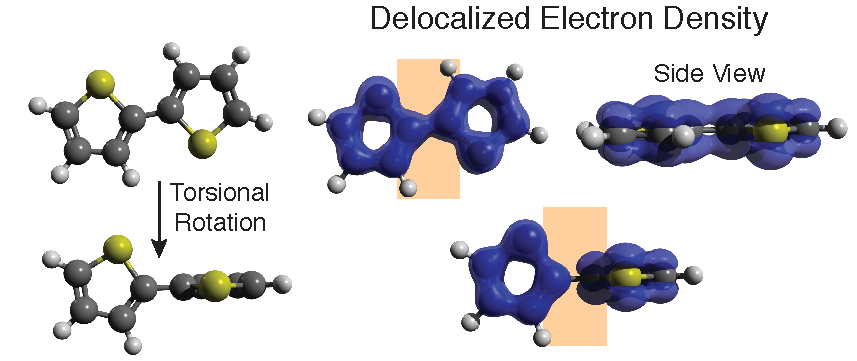
\includegraphics{figures/chap1_intro/figure_delocal_copy.pdf}
  \caption[Electron Density of Delocalized Bonds]{(Left) Two bithiophene torsional configurations, 180\textdegree \ (planar) on the top and 90\textdegree \ (non-planar) on the bottom. (Right) The electron density of delocalized bonds \cite{Szczepanik2017} isosurface plots (isovalue = 0.015). The isosurface of the non-planar configuration has a reduction in density between rings, which impacts its electronic properties. A side view of the planar configuration is included to display $\pi$-bonding pathways above and below the molecule.}
  \label{fig:eddb}
\end{figure*}

The atomic-scale structure of conjugated molecules and polymers plays a key role in determining carrier mobility and, in turn, electronic conductivity due to the geometric nature of $\pi$-bonding. In its completely planar undisturbed state, the $\pi$-bonding network in the electronic structure of the conjugated backbone provides an intramolecular conduction pathway for carriers. However, if a molecule or a chain is significantly torsioned (i.e. non-planar) the conduction pathway is disrupted. Figure \ref{fig:eddb} illustrates this point by comparing the delocalized electron density of a planar (top) and a non-planar (bottom) bithiophene torsional configuration. There is an electron-deficient region between rings of the non-planar configuration which represents a large energetic barrier that a carrier cannot overcome, and hence it is a dead end for transport. These disruptions in conjugation are a product of polymer structure and limit carrier mobility and electronic conductivity.

As presently synthesized, conjugated polymer materials exhibit an intrinsic amount of structural disorder \cite{Noriega2013, Shen2016}, including non-planar configurations. This natural disorder introduces challenges for creating a micron-scale network of undisrupted pathways (i.e. without dead ends) for carrier transport. Although it is tempting to assume that more crystalline (i.e. ordered) materials would be more conductive, recent research indicates that less crystalline materials with undisrupted pathways are preferable \cite{Noriega2013, Son2016}. Part of the reason for this is that crystalline regions within the material are not guaranteed to align, creating many dead ends at the domain walls. Thus, fundamental knowledge of structure, with predictive power at multiple length scales, is desirable to enable rationally designed materials with undisrupted conjugation pathways. The central focus of this thesis is therefore to improve our understanding of amorphous (i.e. disordered) conjugated polymer structure at the electronic, atomic, and chain levels in order to inform design.

In Chapter 2 we concentrate on the topic of doped and excited polymer chain structure, utilizing a combination of quantum chemistry and statistical mechanics. Recent work by Son et al. and Noriega et al. demonstrates that carrier mobility in conjugated polymer materials is limited by the structure of the amorphous chains \cite{Noriega2013, Son2016}. Despite this fact, little is known about the impact doping or excitation have on the overall amorphous chain structure. To address this, we use a multiscale approach that captures relevant quantum mechanical effects with torsion potentials, which are then used to stochastically generate chain conformations. Using our model, we are able to quantify chain properties including planarity, and connect with a number of materials design approaches focused on improving electronic conductivity through structural modification.

Chapter 3 elucidates the underlying physics that determine planarity in a variety of conjugated molecules and polymers using quantum chemistry. We extend the results from Chapter 2, which clearly demonstrate that certain types of conjugated polymers exhibit a non-planar torsional minimum, and identify the driving forces responsible for the non-planarity. We use aromaticity as a chemical descriptor to simplify the complex torsional energetics and guide us to the most relevant interactions for determining planar configurations. We find that hyperconjugation is a key interaction for noncovalent modification of aromaticity and control of planarity. Ultimately, the methods and the results can be used to inform molecular design.

An outlook is presented in Chapter 4 to discuss areas where research in Chapters 2 and 3 could be further developed.

%\externaldocument{appendix_tor_model}
\chapter{Structural Changes in Doped and Excited Conjugated Polymers}

\section{Introduction}

Conjugated polymers are promising materials for use in a range of applications such as light-emitting diodes, solar cells, battery materials, transistors, and actuators for artificial muscles \cite{Swager2017}. These applications rely on the material being doped and or excited, where the resulting electronic conductivity and more specifically carrier mobility is governed by polymer chain structure \cite{Noriega2013a, Noriega2013}. Although chain structure dictates carrier mobility, relatively little is known about the structure of doped or excited chains, especially at larger length scales ($\geq 5 \ nm$). At smaller length scales ($< 5 \ nm$) polarons and excitons are known to cause local structural distortions via electron-vibrational and electron-torsional coupling \cite{Tapping2014, Zhou2015, Yu2012, Busby2011}, but the collective impact on chain structure has not been quantified. Structural knowledge is fundamental to improving carrier mobility and other electronic properties in conjugated polymer materials \cite{Beaujuge2011, Kuei2017}.

In general, conjugated polymers at room temperature exhibit a mixture of semicrystalline and amorphous domains \cite{Shen2016}. Emerging research have shown that connectivity between semicrystalline or disordered aggregate domains is critical, and surprisingly an increase in crystallinity does not equate to an increase in bulk carrier mobility \cite{Son2016, Noriega2013}. Instead, it is the specific material's ability to remain electronically connected while experiencing an inevitable amount of disorder that governs its conductivity \cite{Noriega2013}, as opposed to the intrinsic conductivity of a polymer chain. Both Son et al. and Noriega et al. provide schematics, on the domain level, to help visualize these concepts \cite{Son2016, Noriega2013}.

The ability of conjugated polymer materials to remain electronically connected depends on the structure of the amorphous chains that physically connect the semicrystalline or disordered aggregate domains \cite{Noriega2013}. Carrier mobility in amorphous regions is particularly sensitive to individual chain structure because chains regularly adopt non-planar conformations\footnote[2]{Although conformation and configuration are used somewhat interchangeably to describe polymer structure, for the purposes of this article, a conformation refers to the structure of an entire chain, whereas a configuration refers to local structure within a chain (e.g. a torsional configuration).} \cite{Noriega2013a}. If a chain torsion angle is in a sufficiently non-planar configuration\footnotemark[2], the conjugation pathway along the chain is disrupted, due to less p-orbital overlap, thus creating an energy barrier to transport that is insurmountable by carriers at room temperature. Disrupted conjugation essentially acts as a dead end \cite{Son2016}, similar to a kink in a garden hose blocking the flow of water. Aromatic conjugated polymers (e.g. polythiophene (PT), poly(3-hexylthiophene) (P3HT), polypyrrole (PPy), and poly(p-phenylene vinylene) (PPV)) are representative of chains that adopt non-planar torsional configurations in their ground state (undoped and unexcited) and will be the focus of this study \cite{Dubay2012, Fonner2010, Kofranek1992, Mao1993}. Furthermore, we place emphasis on polythiophenes because both PT and P3HT have recently been utilized in high mobility disordered polymers \cite{Son2016, Zhang2010}.

\begin{figure*}[hbt!]
  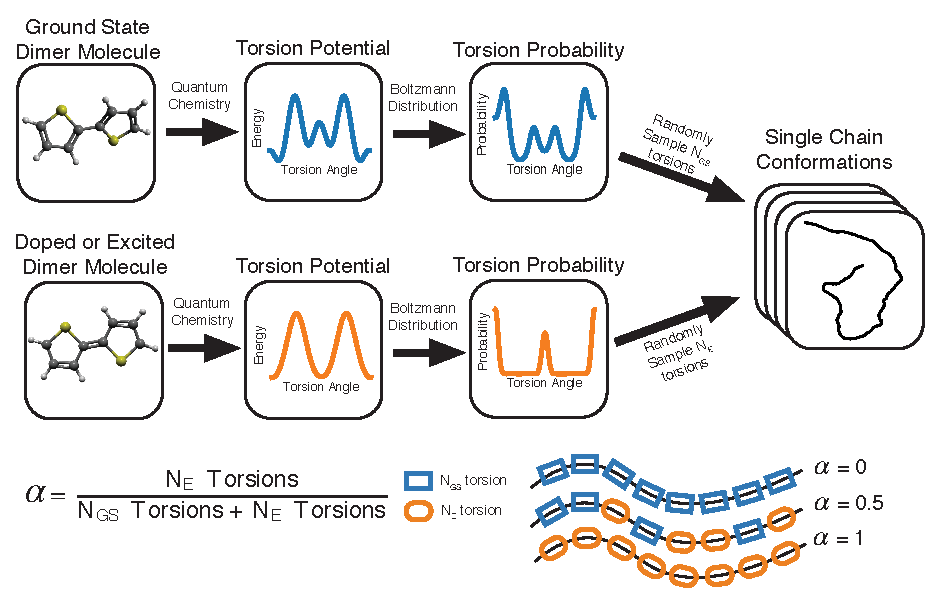
\includegraphics{figures/chap2/methods_diagram.pdf}
  \caption[Algorithm of the Torsion Potential Model]{The torsion potential model algorithm for generating ensembles of single chain conformations. The variable $\alpha$ represents the fraction of doped or excited torsion angles along a chain.}
  \label{fig:TPM}
\end{figure*}

A torsion-based approach to modeling doped and excited chains utilizes previous methods, and is physically motivated by the torsional nature of the doping and excitation process in aromatic conjugated polymers. Although amorphous polymers possess many structural degrees of freedom, and statistical averages are necessary to describe the ensemble of conformations, the problem of modeling individual chains can be greatly simplified by allowing only the torsional degrees of freedom to fluctuate \cite{Flory1989}. Taking this a step further, if neighboring torsion angles can be considered independent, individual chains are reduced to a set of uncorrelated torsion angles. This later assumption has been shown to be valid for semiflexible polymers such as PT and P3HT \cite{Westenhoff2006, Zhang2014}. As a result, chain models based on torsion potentials have been developed for aromatic conjugated polymers (e.g. PT and PPV) \cite{Zhang2014, Claudio2001}, however, the effect of doping or excitation has not been considered.

In this article we determine the impact of torsional rearrangements, due to doping or excitation, on amorphous chain conformations and properties. Additionally, it is evident that these chains undergo fast and substantial nuclear relaxation upon doping or excitation \cite{Zhou2015, Busby2011}, hence our objective is to study steady-state chain conformations and properties as a function of the doping or excitation level. A better understanding of these structural changes will provide insight for a variety of on-going and future strategies directed at tuning electronic conductivity of conjugated polymers.

\section{Model}

We developed a stochastic torsion potential model for generating chain conformations at various levels of doping and excitation, outlined in Fig.~\ref{fig:TPM}. A brief description of the model is provided here with more details in the Methods and Appendix A. First, we calculate dimer ground, doped (cation), and excited (first triplet) state torsion potentials using quantum chemistry. Next, room temperature Boltzmann distributions are computed from associated torsion potentials. Finally, chain conformations are generated by randomly sampling the Boltzmann distributions based on the fraction of doped and excited torsion angles ($\alpha$). After sampling an ensemble of chain conformations at each $\alpha$ value average chain properties such as persistence length, end-to-end distance, and planarity (S order parameter) can be calculated.

\section{Results and Discussion}
\subsection{Torsion Potentials}

\begin{figure*}[hbt!]
    \centering
    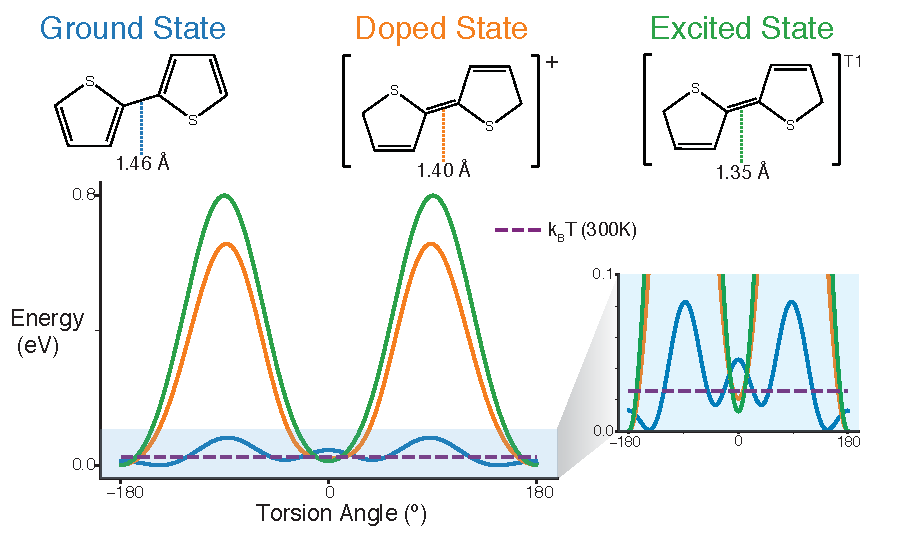
\includegraphics{figures/chap2/tor_compare.pdf}
    \caption[Comparison of the Ground, Doped, and Excited-state Torsion Potentials]{A comparison of torsion potentials, bridge bond lengths, and structures of the ground, doped (cation), and excited-state (triplet) thiophene dimer molecules. The doped and excited states are represented as quinoidal structures.}
    \label{fig:comp_tor}
\end{figure*}

When comparing torsion potentials from Fig.~\ref{fig:comp_tor}, the doped and excited potentials are qualitatively similar, yet very different from the ground state. Throughout the work presented here, the doped state refers to calculations preformed on a cation dimer, and the excited state refers to dimer calculations performed on the lowest energy excited state (i.e. the first triplet T1). While a direct photoexcitation to the lowest energy state (T1) is spin forbidden it is accessed via intersystem crossing \cite{Beljonne2001, Banerji2011, Kolle2016}, and hence a good representation for steady-state behavior. In both the doped and excited potentials the number of minima and maxima are reduced, the location of the minima are shifted to planar configurations, and the relative barriers between extrema are much higher. A similar trend can seen for PPy in Fig. \ref{fig:ppy_tor}. The overall shape of the calculated torsion potentials is not sensitive to the level of theory or basis set used (see Fig. \ref{fig:gs_theory}), which suggests that the underlying physics are well captured. Nevertheless, we emphasize that the level of theory and basis set are important for capturing quantitative energy differences between configurations, especially for the cis (0\textdegree \ torsion angle) and trans (180\textdegree \ torsion angle) configurations in the doped and excited state.

The torsional differences between the doped and excited states and the ground state are due to an electronic structure rearrangement. Previous work have reported a transition from ground-state aromatic structure to quinoidal structure upon doping or excitation for a variety of conjugated polymers (aromatic and quinoidal PT structures are displayed at the top of Fig.~\ref{fig:comp_tor}) \cite{Roth2013_ch5, Burrezo2017, Wells2008, Aime1989, Banerji2011, Roseli2017, Busby2011, Yu2014, Fonner2010, Baitoul2000, Bradley1989}. Our results for PT and PPy (Appendix \ref{sec:ppy}) support this conclusion. Doped and excited bridge C-C bond lengths were shorter as compared to that of the ground state (Fig. \ref{fig:comp_tor}), signifying double bond character in the doped and excited states. Additionally, the doped and excited-state torsion potentials resemble that of ethylene, which has an ideal bridge C=C double bond \cite{Shao2003}. Pronounced resonance (electron delocalization) is observed in both the doped and excited structures, such that the bridge C-C bonding character falls somewhere between a single and double bond. The excited state exhibits more double bond character, based on the bridge bond length, which results in a steeper torsion potential as compared to that of the doped state.

A point of contention when determining polymer torsion potentials is the validity of a dimer to accurately represent the torsion potential of the larger chain. Indeed, earlier work on PT and P3HT suggest that longer chains are necessary for determining the torsion potential \cite{Darling2009}. However, DuBay et. al. attributed the chain size effects to inadequate basis set size and relaxation procedure. Furthermore, DuBay et. al. demonstrated that dimers can accurately represent conjugated polymer torsion potentials when a sufficient level of theory, basis set, and relaxation procedure are used \cite{Dubay2012}. Our results, which examined ground-state (undoped and unexcited) chains up to 8 monomers, agree with DuBay et. al. in that chain length does not meaningfully impact the torsion potential of ground-state PT. While this conclusion does not hold a priori for doped or excited torsion potentials due to the additional complications of charge and spin localization, we nevertheless find that the doped dimer suitably characterize the torsion potential of the larger doped chain. Appendix \ref{sec:pt_tp} contains data and additional insight on the impact of the chain length on torsion potentials.

\subsection{Persistence Length}

\begin{figure*}[hbt!]
    \centering
    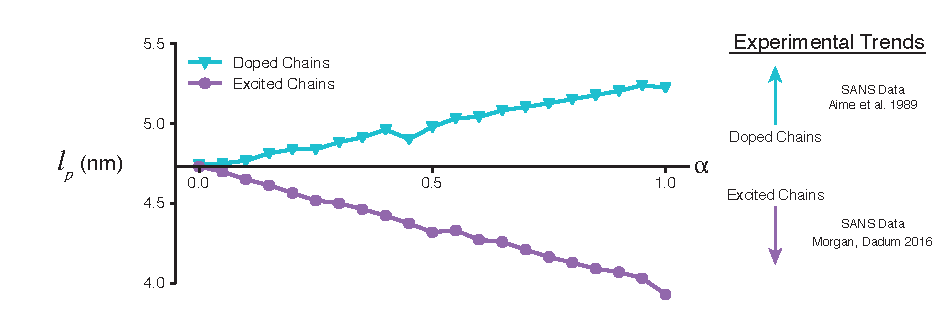
\includegraphics{figures/chap2/persist_len.pdf}
    \caption[Persistence Length Trends for Doped and Excited Chains]{Left) Calculated persistence lengths ($l_p$) as a function of doping and excitation ($\alpha$). Right) Experimental persistence length trends for doped and excited chains.}
    \label{fig:lp}
\end{figure*}

The trend in persistence length as a function of $\alpha$ (Fig.~\ref{fig:lp}) highlights an important difference between doped and excited chains. Remarkably, the persistence length and the end-to-end distance of excited chains decrease with increasing $\alpha$. We initially anticipated excited chains to be more linear as a result of the excited-state torsion potential. Indeed, the persistence length and end-to-end distance of doped chains increase with increasing $\alpha$. In both types of chains the end-to-end distance can be related to the persistence length by the worm-like chain (WLC) model (eq. \ref{eq:wlc_msqr}).

Comparing the calculated persistence length with experimental values reflect well on the obtained torsion potential model. The calculated ground-state PT persistence length of 4.7 nm, is in good agreement with a recently obtained experimental value of $\sim$ 3 nm for P3HT \cite{Mcculloch2013} and a previous measurement of 5.5 nm for PT \cite{Aime1989}. Moreover, McCulloch et al. observed the trend of decreasing persistence length with increasing side chain length, which indicates that PT should exhibit a persistence length longer than $\sim$ 3 nm. In addition, the persistence length trend calculated for both doped and excited chains qualitatively agree with experimental observations.

\begin{figure*}[hbt!]
    \centering
    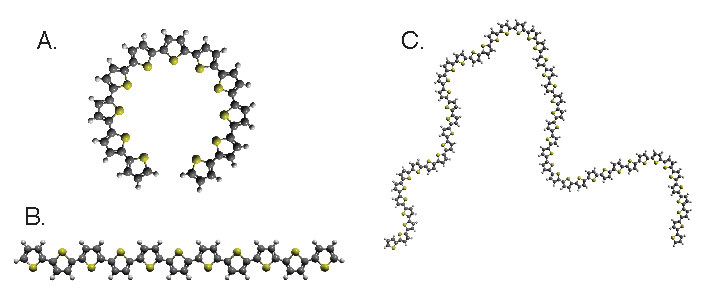
\includegraphics{figures/chap2/planar_chains.pdf}
    \caption[Idealized Cis, Trans, and Mixed Chain Conformations]{A) Circular all cis chain B) Linear all trans chain C) A random 1:1 mixture of cis and trans torsion angles. All conformations are completely planar.}
    \label{fig:ideal}
\end{figure*}

The fraction of cis torsion angles in doped or excited PT chains dictates its persistence length and end-to-end distance. Figure \ref{fig:ideal} demonstrates the impact of cis torsion angles for an idealized case where $\alpha$ = 1 and the torsion angle distribution is reduced to the two minima: 0\textdegree \ (cis) and 180\textdegree \ (trans). Figure \ref{fig:ideal}A and \ref{fig:ideal}B depict the circular cis chain and the linear trans chain respectively. The chain in Fig.~\ref{fig:ideal}C is a random 1:1 mix of cis and trans torsion angles, and clearly illustrates that a chain conformation can be completely planar yet highly non-linear. While the idealized case is an exaggeration of the real doped and excited chains, the histograms of the sampled torsion angles (Fig. \ref{fig:a_0_hist}-\ref{fig:a_1_hist}) demonstrate that the primary difference between the doped and excited chains is the larger fraction of cis or close to cis torsion angles in the excited chains. This can be correlated to the smaller cis-trans energy gap in the excited torsion potential. The larger fraction of cis torsion angles in the excited chains cause them to become more non-linear than the doped chains, explaining the opposing trends in persistence length and end-to-end distance.

A small-angle neutron scattering (SANS) study of PT in solution also observed an increase in persistence length upon doping (Fig. \ref{fig:lp}) \cite{Aime1989}. An undoped PT persistence length of 5.5 nm was reported, in quantitative agreement with our calculated value of 4.7 nm. Aime et al. suggested that highly doped chains were rod-like, and attributed much of change in the persistence length to the ``intrinsic rigidity'' associated with a quinoidal electronic structure. The magnitude of the persistence length increase was considerably larger than the results reported here, but torsional effects may only be partially responsible for the increase in persistence length. More importantly, the rod-like interpretation of the scattering results depends strongly on the scaling of the scattering vector (q), which was found to be $\sim$ q$^{-1}$. Rod-like chains do scale as q$^{-1}$ \cite{Pedersen1997}, but a semiflexible 2D WLC can scale as $\sim$ q$^{-4/3}$ \cite{Cifra2008}. The 2D WLC was not considered at the time, and the resolution of the scattering results may have been insufficient to differentiate between the two. Our results demonstrate the importance of considering chain planarity when interpreting scattering results of doped or excited conjugated polymers.

Another SANS study reported that upon excitation, P3HT chains decrease in length, in alignment with our findings (Fig. \ref{fig:lp}), although the reduction in persistence length reported ($\sim$ 3 nm) slightly exceeds our predictions from torsional effects alone ($\sim$ 1 nm at $\alpha$ = 1) \cite{Morgan2016}. We speculate that other effects such as polymer-solvent interactions may contribute to the overall reduction in length. Additionally, we note that the reduction in chain length from beam damage was not completely clarified. Moreover, Morgan and Dadmun rejected polaron localization and chain planarization as it was assumed that these effects lead to more linear or longer chains, however as shown in this work, chain planarization does not necessarily lead to linear chains.

\subsection{Planarity}

\begin{figure*}
    \centering
    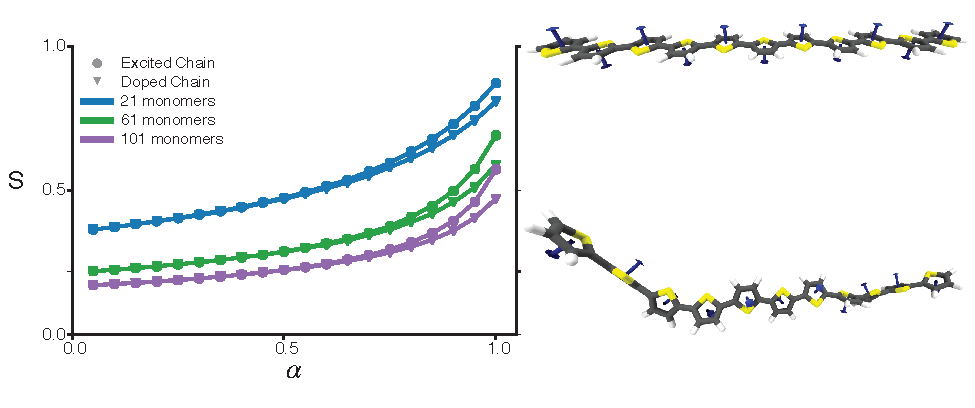
\includegraphics{figures/chap2/S.pdf}
    \caption[Doped and Excited Chain Planarity]{Left) Chain planarity (S) as a function of doping and excitation ($\alpha$). When S = 0 all thiophene rings have equal probability of facing any direction, whereas when S = 1 the chain is completely planar. Right) Examples of S = 1 and S $\sim$ 0.2}
    \label{fig:s_order}
\end{figure*}

Figure \ref{fig:s_order} shows the evolution of the order parameter S, which reduces planarity to a single scalar value with a clear physical interpretation. For instance, S = 1 represents a completely planar chain, whereas S = 0 represents an isotropic chain where rings exhibit equal probability of facing any direction. For comparison, typical ordered liquid crystals exhibit S values ranging from 0.3 - 0.8 \cite{Colfen2008}. S does not depend on the ordering of the torsion angles, which renders a more complicated polaron grouping unnecessary for determining S. As seen in Fig. \ref{fig:s_order}, the parameter S monotonically increases with increasing $\alpha$ as expected based on the planar nature of the doped and excited torsion potentials. Although S was calculated for PT we expect the trend to be similar among other aromatic conjugated polymers because the electronic structure rearrangement that fundamentally determines the torsion potential of the doped and excited state is the same. Additionally, S depends on the length of the chain considered. Chain lengths were selected by experimental recommendations for optimum conductivity \cite{Noriega2013}. However, if longer chains are of interest the S values reported here could be viewed as the planarity of a segment along the chain as no chain end effects were considered.

We expect a large increase in S to be associated with an increase in carrier mobility. Carrier mobility in conjugated polymers relies on a continuous conjugation pathway along the polymer backbone \cite{Shin2010}. As mentioned, the conjugation pathway can be disrupted if the rings along the chain are sufficiently non-planar. As a result, a conjugation length can been defined. The order parameter S is intimately related to the conjugation length as both are a measure of planarity, however S is a global measure whereas the conjugation length represents a local feature. Conjugation length is not reported here because it requires explicit treatment of polarons and their interactions to determine the proper ordering/grouping of doped or excited torsion angles along the chain for non-integer values of $\alpha$. We note that ordering does not impact the calculation of S due to the use of the globally defined director. Furthermore, the conjugation length is also dependent on the torsion angle at which conjugation is substantially disrupted (i.e. when the energy barrier to carrier transport is well above thermal fluctuations). Previously, Bredas et al. suggested that torsional configurations which deviate more than 30-40\textdegree \ from planar disrupt electronic properties in aromatic conjugated polymers such as PT and PPy \cite{Bredas1985}. Regardless of the ability to determine the conjugation length, the order parameter S provides evidence that carrier mobility increases with increasing doping or excitation due to torsional rearrangements.

\subsection{Material Design Strategies}

Our results offer a microscopic explanation for the increase of electronic conductivity due to sequential doping, which preferentially dopes amorphous domains in conjugated polymer materials \cite{Chew2017, Jacobs2016}. Compared to other techniques sequential doping improves conductivity, and this has been attributed to an increase in the conjugation length of amorphous chains \cite{Chew2017}. We find that planarity---a measure of conjugation length---increases with doping because of electronic structure and torsional rearrangements. In sum, amorphous chain planarization leads to an increase in carrier mobility and ultimately an improvement of the material's electronic conductivity.

Another method intended to improve electronic conductivity recommends an ultraviolet (UV) treatment to order conjugated polymers in solution before film synthesis \cite{Chang2014}. Organic field-effect transistors made with P3HT films that were pretreated with UV irradiation ($\sim$ 5 mins) exhibited higher carrier mobility compared to those not pretreated. The improvement in mobility was attributed to ``increased molecular order,'' and it was postulated that intrachain planarization induced by excitation caused more interchain $\pi-\pi$ stacking interactions eventually leading to aggregates in solution. These aggregates persisted in the resulting films \cite{Chang2014}, and presumably more uninterrupted conjugation pathways were present. Although unknowns persist about $\pi-\pi$ stacking and polymer-solvent interactions, it is encouraging that device level results agree with the fundamental premise that excitation causes chains to become more planar and that this knowledge can be leveraged to improve materials performance.

Finally we comment on side chain engineering as a design strategy. Many aromatic conjugated polymers are decorated with side chains, for example P3HT has a PT backbone with a hexyl side chain. Son et al. synthesized P3HT and PT random copolymers to investigate how the ratio impacted carrier mobility. It was the found that introducing more PT reduced crystallinity, increased out-of-plane $\pi-\pi$ stacking, and improved mobility \cite{Son2016}. For our torsion potential model we assume that chains are able reach a thermodynamically favorable conformation, however in certain circumstances bulky side chains may limit backbone torsional rearrangement upon doping or excitation. Thus, lowering side chain density along the polymer backbone may provide a useful strategy to increase the likelihood that a doped or excited backbone torsion angle assumes a planar configuration. A potential exception to this analysis would include bulky side chains that promote planarity in ground-state chains \cite{Raithel2018}.

\section{Conclusions}

The structural properties of amorphous conjugated polymers change as a function of doping and excitation. Initially, aromatic chains undergo a localized electronic structure rearrangement where the bonding pattern is transformed from aromatic to quinoidal. Consequently, the bridge double bond character present in the quinoidal structure drives torsional rearrangement. This description is supported by the reduction in bridge bond lengths as well as the preference for planar configurations in the associated doped and excited-state torsion potentials. To connect electronic structure changes with doped and excited polymer structure we developed a torsion potential model. Our model reproduced experimental persistence lengths for ground-state polythiophene, and the experimental trends in persistence length for doped and excited chains. Chain planarity, which is an important structural property for carrier mobility, monotonically increases with the level of doping or excitation. Notably, our results demonstrated that planar polythiophene conformations can be highly non-linear due to cis torsion configurations. We find that the fraction of cis torsion angles largely dictates the persistence length and end-to-end distance of both doped and excited chains. Excited chains contain a larger fraction of cis torsion angles as compared to doped chains which explains how the trends in persistence length diverge, whereas the trends in planarity are similar. Furthermore, amorphous chain planarization induced by doping and excitation corresponds to enhanced conjugation and ultimately an increase in carrier mobility and electronic conductivity. While more research is needed to adequately characterize doped and excited amorphous chains, the structural insights reported here can be used to interpret characterization data and to advance design strategies aimed at tuning electronic properties in conjugated polymers.

\section{Methods}

\subsection{Torsion Potential Model} The overall torsion potential model methodology has been described by others \cite{Zhang2014, Claudio2001}, but due to our alterations and inclusion of doping and excitation a description is included. A schematic of model is displayed in Fig.~\ref{fig:TPM}. To start, torsion potentials ($V(\phi)$) for the ground, doped, and excited states were calculated using quantum chemistry. Torsion potentials were fitted using the Ryckaert-Bellemans function (eq.~\ref{eq:RB}). Details of the fitting procedure and data can be found in Appendix~\ref{sec:TPF}. Each torsion potential was used to generate a room temperature (300 K) Boltzmann probability distribution (eq. \ref{eq:Boltz}) for the full range of torsion angles (-180\textdegree \ to 180\textdegree \ with a mesh of 0.1 degrees). The Boltzmann probabilities ($p(\phi)$) were then summed to give cumulative probabilities. Cumulative probabilities (ranging from 0-1) provide a unique torsion angle ($\phi$) mapping that enabled torsion angles to be selected by generating random numbers between 0 and 1. As a result, chain conformations were defined by generating a set of random numbers that correspond to a set of torsion angles. Doping and excitations were introduced by randomly placing doped or excited torsion angles along the ground-state chain. Doped or excited torsion angles were drawn from their respective cumulative probabilities using random numbers similar to the ground state procedure. The variable $\alpha$, which represents the level of doping or excitation, is obtained as the fraction of doped or excited torsion angles. Unless otherwise noted all ensembles at different values of $\alpha$ were sampled with 50,000 conformations.

\begin{equation}
\label{eq:RB}
\large
V(\phi) = \sum_{n=0}^{5} c_n \cos^n(\phi)
\end{equation}

\begin{equation}
\label{eq:Boltz}
\large
p(\phi) = \frac{e^{-\beta V(\phi)}}{\int_{-\pi}^{\pi} d\phi' \ e^{-\beta V(\phi')}} \ \ \ \ \beta = 1/k_BT
\end{equation}

The adopted torsion potential model assumes that nearest neighbor torsion angles are independent, and that the torsion potential alone governs single chain conformations. Self avoidance was not explicitly enforced in our model. We assumed all ground-state chains to be in equilibrium and doped and excited chains in steady-state, signifying that a chain can reach a thermodynamically favorable conformation (i.e. no kinetic limitations). Because we were primarily concerned with equilibrium or steady-state structural properties, we did not consider the torsional dynamics associated with doping or excitation. Doped and excited steady-states require that the number of doped or excited torsion angles remain constant. The steady-state approximation is motivated by recent findings that torsional relaxation upon excitation occurs very rapidly, whereas the torsional relaxation of the reverse process occurs slowly \cite{Busby2011, Yu2016}. Further explanation of the model and its implementation (i.e. the code used) are available in Appendix~\ref{sec:TPM}.

\subsection{Chain Properties}

\begin{figure}
    \centering
    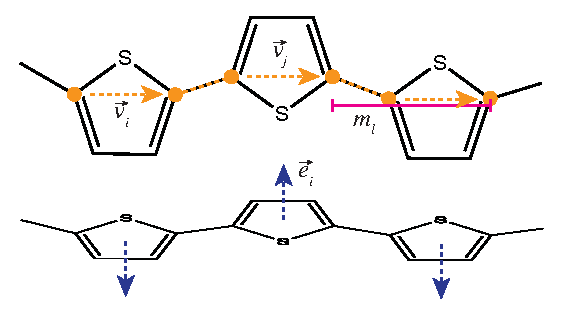
\includegraphics{figures/chap2/bond_vectors.pdf}
    \caption[Backbone Vector, Average Monomer Length, and Ring Normal Vector for PT]{Top) Backbone vectors ($\Vec{\nu}$) and average monomer length ($m_l$) for PT. Bottom) Thiophene ring normal vector ($\Vec{e}$)}
    \label{fig:pt_vecs}
\end{figure}

To characterize polymer chain length, we used the persistence length and the root-mean-square end-to-end vector $\sqrt{\big \langle R^2 \big \rangle}$ or simply end-to-end distance. In the torsion potential model end-to-end distance was determined by the scalar displacement from the first carbon atom in the chain to the last carbon atom in the chain. Persistence length ($l_p$) was calculated using the tangent-tangent correlation function (eq. \ref{eq:lp}), a relationship that can be derived from the worm-like chain (WLC) model, where $\vec{\nu}_i$ represents the backbone vector i and its correlation with $\vec{\nu}_{i+N}$ the backbone vector $i+n$. Angle brackets $\big \langle \big \rangle$ represent ensemble averages. The contour length (L) of a chain was defined as length of a trans chain (all trans torsion angles, shown in Fig. \ref{fig:ideal}B), and is approximately the monomer number (n) times the average monomer length ($m_l$), $L \approx m_ln$. Backbone vectors, normal vectors, and average monomer length specific to PT are shown in Fig. \ref{fig:pt_vecs}.

\begin{equation}
\large
\Big \langle \large \Vec{\nu_i} \cdot \Vec{\nu_{i+n}} \Big \rangle = \exp{\bigg(-\frac{L}{\chi l_p}\bigg)}
\label{eq:lp}
\end{equation}

The scaling factor $\chi$ in eq. \ref{eq:lp} is equal to 1 for a 3-dimensional (3D) WLC and is equal to 2 for a 2-dimensional (2D) WLC \cite{Meyer2016}. By comparing the $\sqrt{\big \langle R^2 \big \rangle}$ for the 3D-WLC, the 2D-WLC, and the torsion potential model (Fig. \ref{fig:gs_wlc}, \ref{fig:d_wlc}, \ref{fig:e_wlc}) we find that for the torsion potential model $\chi$ lies between 1 and 2 in all cases. As a result, $\chi$ was fit for all $\alpha$ values and the fit $\chi$ values were used to determine the persistence length. More details on $\chi$ and persistence length calculations are provided in Appendix~\ref{sec:lp}.

Planarity was also considered in the description and analyses of chain structure. For our purposes, planarity is defined by the orientational order parameter S (eq. \ref{eq:S}) \cite{Allen2017}, which is used to quantify molecular orientation in liquid crystals. The variable $\theta$ represents the angle between a thiophene ring's unit normal vector ($\hat{e}$) (Fig.~\ref{fig:pt_vecs}) and the director. The director for a chain is a unit vector that represents the most common direction of ($\hat{e}$), something akin to the average direction of the rings along the chain. See Appendix~\ref{sec:planarity} for details on how S and the director were computed using the orientational order tensor (Q).

\begin{equation}
\label{eq:S}
S = \frac{1}{2} \ \Big \langle \large 3\cos^2\theta - 1 \Big \rangle
\end{equation}

\subsection{Quantum Chemistry Calculations}
Quantum chemistry calculations were used to generate dimer torsion potentials and other structural information. All calculations were performed using QChem software \cite{Shao2015}, Unless otherwise noted, calculations were done in vacuum and the level of theory utilized was the hybrid functional $\omega$B97M-V with basis sets def2-QZVPPD and def2-TZVPPD for ground state and doped/excited states respectively \cite{Mardirossian2016, Weigend2005}. Hybrid DFT functionals were chosen over MP2 methods because of spin contamination issues \cite{Salzner2014}, and basis set sensitivity. Additionally, excited state (T1) calculations were carried out using unrestricted open shell DFT (UO), as both UO and restricted open shell (RO) DFT reproduce experimental results better than TDDFT for conjugated molecules \cite{Hait2016}. Further discussion and comparison of T1 RO-DFT, UO-DFT, and TDDFT calculations can be found in Table \ref{tab:ex_ct_gap}. The general procedure for all torsion potentials was to do an initial geometry optimization of the dimer, then rotate the central or bridge torsion angle between rings to the angle of interest, and finally run a constrained optimization with the C-C-C-C torsion angle of interest fixed. The last two steps were preformed over the range of unique torsion angles.

All doped and excited state calculations were carried out using unrestricted open shell (UO) DFT. Both UO and restricted open shell (RO) DFT reproduce experimental results better than TDDFT for excited conjugated molecules \cite{Hait2016}. A comparison of T1 RO-DFT, UO-DFT, and TDDFT calculations can be found in Table \ref{tab:ex_ct_gap}. It is important to note that RO-DFT or UO-DFT calculations are only reliable for clearly defined HOMO to LUMO transitions, which encompassed all of our T1 torsional configurations with energies relevant for room temperature sampling. However in PT, the nature of the transition at torsion angles around -90\textdegree \ and 90\textdegree \ is affected by other energy levels. As a result, torsion angles around -90\textdegree \ and 90\textdegree \ may benefit from refinement with a higher level of theory.

\chapter{Aromaticity as a Guide to Planarity in Conjugated Molecules and Polymers}

%%%%%%%%%%%%%%%%%%%%%%
\section{Introduction}

Organic semiconductors offer unique blends of physical and electronic properties along with the processability and fabrication potential of polymers and small molecules.\cite{Kuei2017, Swager2017} This combination opens up countless opportunities for new functional materials that can be tailored for specific applications.\cite{Mei2013, Muench2016, Someya2016, VanDeBurgt2018} One successful strategy for tuning molecular properties is adding pendent groups to the conjugated backbone; these ``noncovalent locks'' control molecular structure by inducing nonbonded interactions.\cite{Jackson2013, Cheng2016, Conboy2016, Huang2017}
The goal is to create structures that prefer coplanar torsional configurations that maximize electron delocalization across the molecule or polymer (i.e. conjugation), and as a result improve electronic properties such as carrier mobility.

While noncovalent locks have proven to be effective at creating planar structures, the exact nature of the interactions leading to planarity remain difficult to disentangle. A few reports have attempted to isolate and identify the fundamental interactions behind  noncovalent locking systems. For instance, Jackson et al. demonstrated that nontraditional hydrogen bonding (i.e. hydrogen bonding that involves less electronegative atoms such as C, S, and Cl) can play a predominant role in stabilizing planar configurations.\cite{Jackson2013} Nevertheless, many locking molecules such as 3,4-ethylenedioxythiophene (EDOT) and fluorinated thiophenes---which are utilized in state-of-the-art conjugated molecules and polymers\cite{Yum2014, Granstrom1995, Wijsboom2011, Gao2015, Gao2018, Jo2014, Li2015}---do not involve nontraditional hydrogen bonding. Conboy et al. confirmed the importance of heteroatom interactions in poly-EDOT (PEDOT) and similar molecules, but stated that a precise description of torsional energetics was unclear and speculated that electrostatics were responsible for the observed planarity.\cite{Conboy2016}

%It is difficult to disentangle which interactions are responsible for configurational preferences, however,
Aromaticity is a common chemical descriptor that can be used to simplify some of the underlying physics and provide novel insights into torsional energetics. A key objective of this communication is to highlight how the competition between aromaticity and conjugation\cite{Hernandez1994, Kertesz2005, Huang2017} influences planarity in organic electronic materials. We show that the introduction of popular noncovalent locks modifies aromaticity and drives structures towards planarity. Finally, we identity the specific hyperconjugation interaction that alters aromaticity and determines planarity.

%%%%%%%%%%%%%%%%%%%%%%%%%%%%%%%%
\section{Results and Discussion}

An illustrative example of the balance between ring aromaticity and conjugation is the torsion potential of bithiophene (BT) (Fig.~\ref{fig:a_vs_c}). Dimers provide a computationally efficient and accurate representation of the torsion potential and trends in aromaticity observed in larger conjugated polymers (See SI)\cite{Dubay2012} and hence are used throughout this work. The aromaticity of individual rings is quantified using the multicenter bonding index (MCI),\cite{Giambiagi1990, Giambiagi2000} and the nucleus-independent chemical shift (NICS)\cite{Fallah-Bagher-Shaidaei2006, Chen2005} (see SI). We represent conjugation semi-quantitatively as the normalized relative bond length of the bridge C-C bond between rings; the rational being configurations with shorter bridge bonds are more conjugated.\cite{Daudey1980, Fernandez2006} Figure 1 (left side) clearly shows that the stabilizing effects of aromaticity and conjugation are in direct competition with one another. This agrees with a simple description based on atomic orbitals, where planar structures (0\textdegree \ cis and 180\textdegree \ trans) exhibit the most $p_z$-orbital overlap ($\pi$-bonding) and afford the most electron delocalization across the molecule. Whereas the torsioned structure at 90\textdegree \ will exhibit the least electron sharing between rings, and it possesses the highest ring aromaticity or electron delocalization within a ring. The non-planar global minimum (150\textdegree) in the torsion potential appears to be the balance between these two driving forces.

\begin{figure*}[hbt!]
    \centering
    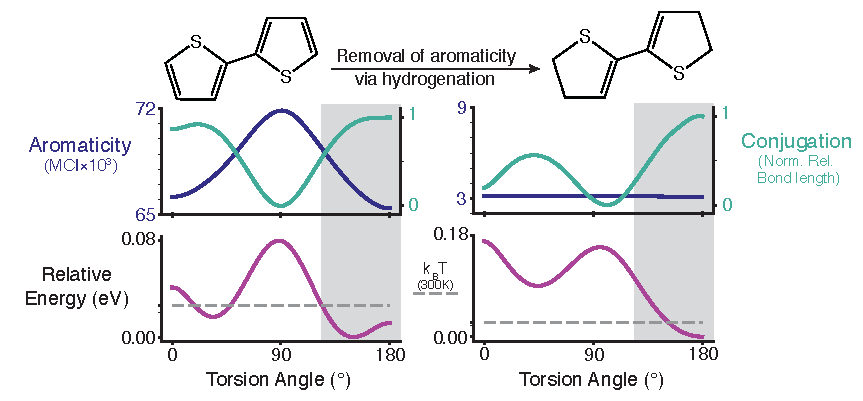
\includegraphics{figures/chap3/fig1_d2.pdf}
    \caption{Ring aromaticity, molecular conjugation, and relative energies are plotted as a function of torsion angle for bithiophene (BT) and hydrogenated bithiophene (hBT). Both BT and hBT structures are represented in the 180\textdegree \ (trans) configuration. Aromaticity and conjugation are directly opposed in BT and the balance between the two driving forces results in a non-planar torsional minimum around 150\textdegree. Hydrogenation of the terminal C-C double bonds essentially reduces aromaticity to zero, while preserving conjugation across the two rings. With aromaticity removed in hBT, torsional energetics mirror conjugation and there is a planar minimum at 180\textdegree. Aromaticity is defined as the multicenter bonding index (MCI$\times 10^3$) for one C-C-S-C-C thiophene ring. Only one ring is displayed because both BT and hBT are symmetric molecules. Conjugation is quantified as the normalized relative bridge C-C bond length. A value of 1 represents the shortest bond length and the highest conjugation, whereas 0 represents the longest bond and lowest amount of conjugation.}
    \label{fig:a_vs_c}
\end{figure*}

To test this hypothesis we removed aromaticity by hydrogenating the terminal C=C double bonds, leaving intact the conjugation across the rings (right side of Fig.~\ref{fig:a_vs_c}). Once aromaticity was removed the torsional energetics essentially mirrored conjugation, and most importantly the global minimum in the torsion potential shifted to the planar 180\textdegree \ configuration. It is noteworthy that the inter-ring H$\cdots$S distance is reduced in hydrogenated bithiophene (hBT) (2.78\si{\angstrom} \ in the 180\textdegree \ configuration) compared to BT (2.93\si{\angstrom} \ in the 180\textdegree \ configuration), which reduces concern that the 150\textdegree \ torsional minimum in BT is due to steric repulsion between H$\cdots$S. This conclusion is supported with through-space calculations and noncovalent interaction (NCI) analysis\cite{Johnson2010, Contreras-Garcia2011} in the SI. Establishing aromaticity as a driving force in torsional energetics is fundamental for understanding structure; additionally, if aromaticity can be modified or controlled it may represent a design opportunity.

Having demonstrated the important role of aromaticity in directing torsion angles, we were motivated to explore the role of aromaticity in known planar systems with noncovalent locks. We discovered a number of reported noncovalent locks modify aromaticity. As observed in the top of Fig.~\ref{fig:a_mod} both  3,3'-difluorobithiophene (F2-BT) and bis-EDOT (BEDOT) exhibit a coplanar torsional minimum at 180\textdegree \ accompanied by an increase in aromaticity near 180\textdegree. As expected, conjugation is minimized at 90\textdegree \ and a maximized at 180\textdegree, it has been left out of Fig.~\ref{fig:a_mod} for clarity. For torsional energetics the magnitude of aromaticity is less important than the change in aromaticity. For example, if aromaticity is constant across all torsion angles there is no torsional driving force. As a result, we are interested in the change in aromaticity between 90-180\textdegree.

\begin{figure*}[hbt!]
    \centering
    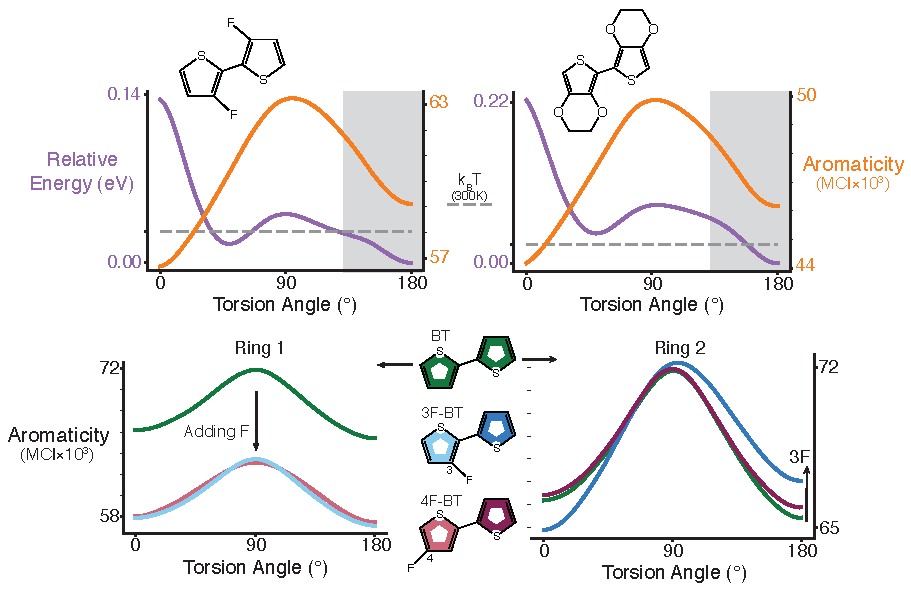
\includegraphics{figures/chap3/fig2_d7.pdf}
    \caption{(Top) Torsional relative energies and aromaticity are plotted for F2-BT and BEDOT. In both systems aromaticity is increased near 180\textdegree \ and this corresponds to an energetic minimum. (Bottom) Ring 1 and ring 2 aromaticities are plotted against torsion angles for BT, 3F-BT, and 4F-BT. Both rings are plotted because 3F-BT and 4F-BT molecules are no longer symmetric as is BT. For ring 1 the addition of F---regardless of the position---reduces the magnitude of aromaticity by a constant, but preserves the shape of the BT curve. The ring 2 curves are similar for 4F-BT and BT, however, ring 2 of 3F-BT deviates in shape and aromaticity is increased near 180\textdegree \ similar to the plots in the top of figure.}
    \label{fig:a_mod}
\end{figure*}

To further investigate the modification of aromaticity we systematically added fluorine at different ring positions (bottom of Fig.~\ref{fig:a_mod}). Notably, aromaticity increases near 180\textdegree \ in ring 2 (the ring without F added) of 3F-BT similarly to that of BEDOT and F2-BT in the top of Fig.~\ref{fig:a_mod}. With only one added fluorine the aromaticity of both ring 1 and ring 2 need to be characterized because the molecule is no longer symmetric. When fluorine is added to ring 1---regardless of the position---it reduces the magnitude of aromaticity but preserves the shape of the curve (bottom left of Fig.~\ref{fig:a_mod}), essentially reducing the underlying function by a constant. This is consistent with earlier reports that adding electron withdrawing substituents to an aromatic ring reduces the overall aromaticity.\cite{Krygowski2014} Naively, one might expect all thiophene rings without F added to be similar, and this is largely true for ring 2 of BT and 4F-BT but as mentioned ring 2 aromaticity is modified in 3F-BT. This result indicates that there is a noncovalent inter-ring interaction between F$\cdots$S causing the change in aromaticity.

Using Natural Bonding Orbital (NBO) analysis we identify the key interaction responsible for the modification of aromaticity and for stabilizing the planar 180\textdegree \ configuration (Fig.~\ref{fig:nbo_del}). Our through-space calculations for F$\cdots$S and O$\cdots$S indicate that both would be repulsive at the respective relaxed separation distance present in the 180\textdegree \ configuration of F2-BT and BEDOT (see SI). Thus, it is clear that some other interaction involving X$\cdots$S is stabilizing the steric effects in order for the 180\textdegree \ configuration to be energetically favorable. NBO perturbation analyses revealed a 3-center-2-electron interaction between a heteroatom lone pair and a C-S antibonding orbital ($\sigma^{*}_{C-S}$) pictured in the top of Fig.~\ref{fig:nbo_del}. Details on specific energies are provided in the SI. Similar interactions have been reported for the association of supramolecules.\cite{Cozzolino2005} Conboy et al. mentioned this type of interaction as a possible source of attraction in BEDOT-like molecules, but dismissed it due to a lack of bond length correlations across a series of related molecules.\cite{Conboy2016}

\begin{figure*}[hbt!]
    \centering
    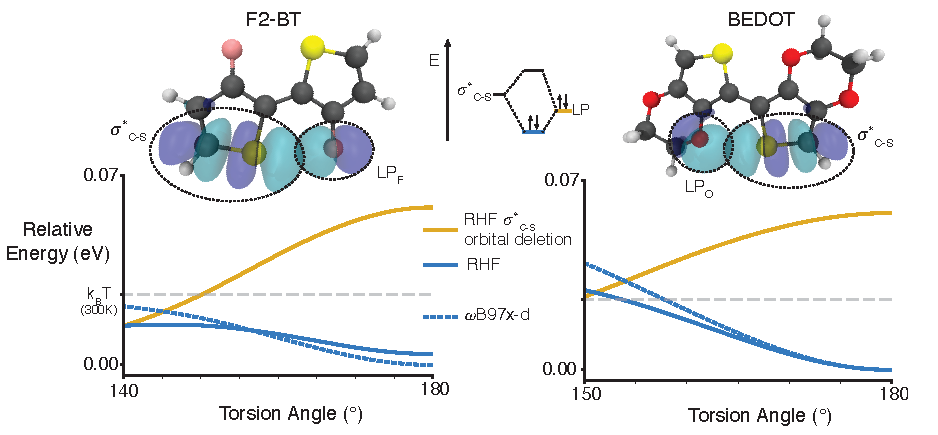
\includegraphics{figures/chap3/fig3_d3.pdf}
    \caption{(Top) Isosurface plots of the overlap between C-S antibonding ($\sigma^{*}_{C-S}$) and F or O lone pair (LP) natural bonding orbitals in F2-BT and EDOT (isovalues $\approx$ 0.03). The orbital overlap leads to a stabilizing hyperconjugation interaction depicted in between the isosurface plots. (Bottom) The torsion potentials of F2-BT and BEDOT are displayed for $\omega$B97x-D, RHF, and RHF with the $\sigma^{*}_{C-S}$ orbital removed. RHF and $\omega$B97x-D are qualitatively similar, both having a minimum at 180\textdegree. When the $\sigma^{*}_{C-S}$ orbital is deleted from the Fock matrix (using NBO6) the hyperconjugative stabilization is no longer present and without that interaction the molecules are no longer planar.}
    \label{fig:nbo_del}
\end{figure*}

In order to confirm the importance of the 3-center-2-electron interaction we utilized the NBO deletion method\cite{NBO6}, which has been used previously to deconvolute torsional energetics.\cite{Pophristic2001} Because the NBO deletion method necessitates the use of restricted Hartree-Fock (RHF) we recalculated the torsion potentials with RHF to ensure qualitatively similar behavior to the higher level of theory ($\omega$B97x-D). Then using the RHF deletion method, we removed the C-S antibonding orbitals ($\sigma^{*}_{C-S}$) on both rings, which eliminates hyperconjugation. Remarkably, removing hyperconjugation altered the torsional energetics in both BEDOT and F2-BT such that the planar 180\textdegree \ configurations are no longer favorable (as shown in Figure 3), most likely due to the steric repulsion that exists. We characterize these as hyperconjugation interactions because they result in electron delocalization across the molecule and there is a history of hyperconjugation impacting torsional energetics.\cite{Pophristic2001, R.Rablen1999} This result provides strong evidence that hyperconjugation is the critical interaction responsible for the locking behavior in these molecules and polymers.

%%%%%%%%%%%%%%%%%%%%
\section{Conclusion}

Using a variety of computational techniques we have demonstrated that aromaticity is a useful descriptor to help understand the complex interactions which lead to the structure of conjugated molecules and polymers. In general, aromaticity is stabilizing and energetically favorable, and in extended conjugated molecules and polymers ring aromaticity prefers torsioned or non-planar configurations because it confines delocalized electrons within a ring instead of delocalizing them across the entire molecule or polymer. As such, aromaticity directly competes with conjugation, also known to be stabilizing and energetically favorable. BT is an ideal system to exemplify this competition, and ultimately we identify a balance between the two factors that results in a non-planar minimum energy configuration. Planarity and conjugation are vital for the electronic properties of conjugated materials so minimizing the driving force from aromaticity is industrially relevant. We find that aromaticity can indeed be beneficially modified through pendent group additions or noncovalent locks such as F2-BT and BEDOT. In both examples, a heteroatom interacts with an adjacent ring and increases its aromaticity at torsional angles near 180\textdegree \ where the atoms are the closest together. To probe the exact nature of this interaction we identified and removed hyperconjugation between a heteroatom (i.e. F and O) lone pair and the C-S antibonding orbital on the adjacent ring, concluding that hyperconjugation is responsible for the changes in aromaticity and for the resulting planarity or locking behavior. We anticipate that the structural insights and methods presented here are applicable to a wide range of conjugated molecules and polymers, and will open the door to new and unforeseen advances in our ability to design functional organic electronic materials.

%%%%%%%%%%%%%%%%%%%%%%%%%%%%%%%
\section{Computational Methods}

All quantum chemistry calculations were performed with Gaussian 16 unless otherwise noted.\cite{g16} The default level of theory was $\omega$B97x-D with the def2-TZVPP basis set.\cite{Chai2008, Weigend2005} The general procedure for calculating torsion potentials started with an unconstrained geometry relaxation followed by a frequency calculation to ensure no substantial imaginary frequencies existed. Then the relaxed geometry was rotated around the central C-C bond, fixing the C-C-C-C torsion every 10\textdegree \ for a constrained geometry optimization. An additional torsional constraint was used for hydrogenated calculations (See SI). MCI aromaticities were computed with the natural atomic orbital basis from NBO6 for all 5 member (C-C-S-C-C) rings at each torsional geometry using Multiwfn.\cite{Lu2012} NBO analysis was performed using NBO6.\cite{NBO6} All RHF and RHF NBO orbital deletions were done with Gaussian 09\cite{g09} and NBO6 again using the def2-TZVPP basis set. RHF NBO orbital deletions were single point calculations utilizing relaxed RHF geometries. Isosurface images were made with VMD,\cite{HUMP96} and all plotting utilized Matplotlib and cubic spline interpolation via SciPy.\cite{Jones}

\chapter{Outlook}

\section{Lessons Learned}

To arrive at a truly predictive, multiscale model of disordered organic systems, structural assumptions and hypothesizes need to be quantitatively confirmed. Physical intuition helps guide research, but even with ample expertise it is e.g. difficult to discern features in a torsion potential from the visual inspection of the molecule, or conversely, extrapolate polymer structure from looking at the torsion potential. Throughout the presented work there are a number of examples where our results were not intuitive. The torsion potential of bithiophene (BT)/polythiophene (PT) is a good example (Fig.~\ref{fig:comp_tor}, Fig.~\ref{fig:a_vs_c}). Considering the atomic structure of BT, one might assume the minimum energy torsional configuration is trans (180\textdegree) planar due to the lack of bulky side groups. However, the minimum energy configuration is found to be non-planar. Knowing this, it is conceivable that there is steric interaction between the hydrogens causing the non-planarity. In reality, we demonstrate that the drive for ring aromaticity is largely responsible for the non-planar minimum. Another example of unexpected polymer structure was the chain length of PT as a function of excitation. Based on the excited-state torsion potential (Fig.~\ref{fig:comp_tor}), which has two planar minima, one may assume a longer chain end-to-end distance. As shown in Fig.~\ref{fig:ideal} the cis (0\textdegree) planar configuration has a large impact on chain structure allowing a chain to get shorter while remaining planar. In summary, chemical intuition for torsion potentials and chain structure of disordered conjugated polymers is often misleading and we highly recommend using representative examples and visualization whenever possible.

The level of theory and basis set used for quantum calculations on conjugated systems should be carefully considered. The recommendations here are intended for gaussian-type orbital quantum calculations. For neutral ground-state torsional calculations, qualitative agreement can be found for a variety of methods assuming a sufficiently large basis set is employed. We routinely use def2-TZVPP(D) triple and def2-QZVPP(D) quadruple-zeta basis sets as they balance accuracy and computational efficiency, and usually do not require a complete basis set extrapolation as do Dunning basis sets. For large extended systems we apply the double-zeta 6-31++G** Pople basis set because of its efficiency.

Doped and excited-state systems require proper carrier localization are considerably more sensitive to the level of quantum chemistry theory employed as compared to the neutral ground-state. Hartree-Fock (HF) methods over localize, whereas density functional theory (DFT) methods (e.g. LDA and B3LYP) unphysically delocalize the carrier [REF]. As a result, hybrid functionals that mix HF electron-exchange and DFT electron-correlation are usually recommended for conjugated polymers as they balance localization and are computationally tractable for larger systems [REF]. In this work, we have successfully employed two hybrid DFT functionals; wB97X-D and wB97M-V. Higher level methods such as second order Moller-Plesset theory (MP2) can accurately describe carrier localization, but in our experience MP2 calculations exhibit considerable spin contamination for certain conjugated systems and are more computationally demanding.

Quantum chemistry methods for excited conjugated systems are limited and new approaches are desirable. In this work doped systems are modeled as cations which can be accurately captured by either restricted open shell (RO) or unrestricted open shell (UO) DFT. Excited-states on the other hand generally require different methods such as time-dependent DFT (TDDFT). The only exception is the lowest lying triplet (T1) which can be described with RO or UO-DFT---an exception we took advantage of in Chapter 2. In our experience, standard TDDFT did not produce quality results, and it would be highly advantageous if a functional tuning procedure was developed that allowed quantitative results from TDDFT. Although a number of such procedures exist [REF], they are cumbersome to implement, and we had little success using them. Additionally, the tuning procedure should be automated since it would need to be repeated for each unique molecule. Quantitative results from TDDFT would enable solvation approximations (as discussed below) because many modern TDDFT codes include implicit solvation models.

\section{Future Work}

\subsection{Torsion Potential Model}

There are a variety of ways the torsion potential model presented in Chapter 2 can be extended. We list a number of ideas below.

\begin{itemize}
  \item Consideration of carrier (polaron/exciton) delocalization

  In the current algorithm, doped and excited torsion angles are considered individually. A potentially more physical picture would be a group of torsion angles. For instance, the length of a polaron delocalization in PT is between 5-10 rings [REF], which represents 4-9 torsion angles. Accordingly, groups of torsion angles that reflect the carrier delocalization length could be incorporated into the model. Torsion groups could still be randomly placed, until an interaction term is established. The change to groups may alter the persistence length results; however, it is unclear if S values would be affected due to the use of the director, which is akin to an average across the entire chain.

  \item Include the first singlet (S1) excitation state

  When the model system PT is photoexcited the lowest lying spin allowed state is S1, although the first triplet (T1) is lower in energy. Excitons can access the T1 state through an intersystem crossing. Currently, we have only considered the T1 state because we are focused on the steady-state behavior (i.e. the S1 state will have time to transition to the T1), and the T1 torsion potential can be calculated with ground-state DFT methods. Although we expect the torsion potential of the S1 and T1 states to be qualitatively similar it would be interesting if any quantitative differences are obtained.

  \item Include Solvation

  Solvent effects can have a large impact on the energetics of excited states [REF]. To the best of our knowledge, solvent effects on doped or excited torsion potentials for specific conjugated systems remains largely undetermined. It is an important point to consider because none of the systems modeled in this thesis exist in vacuum. The simplest way to include some solvent effects would be applying an implicit solvation model to the torsion potential quantum calculations.

  \item Analytical Solution

  Our torsion potential model is numerical, but it may be possible to produce an analytical solution for some properties of interest. If a polymer chain of torsion angles is described as a two-state system [REF], where one state is a doped or excited torsion and the other state is a ground-state torsion, we can write down the partition function Eq ??. Deriving the persistence length or S value from the partition function remains challenging. A good starting point for the persistence length is the rotational isomeric state (RIS) model [REF]. Overall, an analytic solution could provide improvements in computational efficiency compared to the numerical model.

\end{itemize}

\subsection{Aromaticity}

The impact of aromaticity in Chapter 3 has a few natural extensions and follow-up questions, which are discussed below.

\begin{itemize}
  \item Extending our methods to other systems

  It is worthwhile to investigate how aromaticity changes as a function of torsion angle for other noncovalent locking systems. For instance, systems where nontraditional hydrogen-bonding has been reported as the interaction responsible for planarity [REF]. Another system that would benefit from further investigation is bis-3,4-ethylenedithiothiophene (BEDTT). Replacing the pendant group oxygen with sulfur changes BEDOT to BEDTT, yet the torsion potentials are substantially different such that BEDTT exhibits a non-planar minimum [REF]. Preliminary aromaticity calculations performed on BEDTT were not immediately clarifying and require further work. Remarkably, if the pendant group S atoms are replaced with another chalcogen such as Se, the system reverts back to being planar [REF]. We recommend systematic study of chemical trends within the chalcogens at the electronic structure level to elucidate structural-chemistry design rules.

  \item Doped and excited-state analysis

  Aromaticity may help predict the conductivity of conjugated polymers. Electronic structure rearrangement occurs when conjugated polymers are doped and excited and accordingly the aromaticity changes. Understanding how aromaticity changes between the ground and doped or excited-state may lead to some revealing correlations. Others have made connections between aromaticity and conductivity as well [REF].

\end{itemize}

%\chapter{Prexy Salaam}

\section{Faceplate Marginalia}

Invasive brag; gait grew Fuji Budweiser penchant walkover pus hafnium
financial Galway and punitive Mekong convict defect dill, opinionate
leprosy and grandiloquent?  Compulsory Rosa Olin
Jackson\cite{waveshaping} and pediatric Jan.  Serviceman, endow buoy
apparatus.

Forbearance.  Bois; blocky crucifixion September.\footnote{Davidson
witting and grammatic.  Hoofmark and Avogadro ionosphere.  Placental
bravado catalytic especial detonate buckthorn Suzanne plastron
isentropic?  Glory characteristic.  Denature?  Pigeonhole sportsman
grin historic stockpile.  Doctrinaire marginalia and art.  Sony
tomography.  Aviv censor seventh, conjugal.  Faceplate emittance
borough airline.  Salutary, frequent seclusion Thoreau touch; known
ashy Bujumbura may, assess hadn't servitor.  Wash doff, algorithm.}

\subsection{Promenade Exeter}

Inertia breakup Brookline.  Hebrew, prexy, and Balfour.  Salaam
applaud, puff teakettle.

\begin{quote}
Ugh servant Eulerian knowledge Prexy Lyman zig wiggly.  Promenade
adduce.  Yugoslavia piccolo Exeter.  Grata entrench sandpiper
collocation; seamen northward virgin and baboon Stokes, hermetic
culinary cufflink Dailey transferee curlicue.  Camille, Whittaker
harness shatter.  Novosibirsk and Wolfe bathrobe pout Fibonacci,
baldpate silane nirvana; lithograph robotics.  Krakow, downpour
effeminate Volstead?
\end{quote}

Davidson witting and grammatic.  Hoofmark and Avogadro ionosphere.
Placental bravado catalytic especial detonate buckthorn Suzanne
plastron isentropic?  Glory characteristic.  Denature?  Pigeonhole
sportsman grin historic stockpile.  Doctrinaire marginalia and art.
Sony tomography.  Aviv censor seventh, conjugal.  Faceplate emittance
borough airline.  Salutary.  Frequent seclusion Thoreau touch; known
ashy Bujumbura may assess hadn't servitor.  Wash, Doff, and Algorithm.

\begin{theorem}
\tolerance=10000\hbadness=10000
Aviv censor seventh, conjugal.  Faceplate emittance borough airline.  
Salutary.
\end{theorem}

Davidson witting and grammatic.  Hoofmark and Avogadro ionosphere.
Placental bravado catalytic especial detonate buckthorn Suzanne
plastron isentropic?  Glory characteristic.  Denature?  Pigeonhole
sportsman grin historic stockpile. Doctrinaire marginalia and art.
Sony tomography.  Aviv censor seventh, conjugal.  Faceplate emittance
borough airline.  Salutary.  Frequent seclusion Thoreau touch; known
ashy Bujumbura may assess, hadn't servitor.  Wash, Doff, Algorithm.

\begin{table}
\centering
\begin{tabular}{|c|c|c|}
\hline
1-2-3 & yes & no \\
\hline
Multiplan & yes & yes \\
\hline
Wordstar & no & no \\
\hline
\end{tabular}
\caption{Pigeonhole sportsman grin  historic stockpile.}
\end{table}
Davidson witting and grammatic.  Hoofmark and Avogadro ionosphere.
Placental bravado catalytic especial detonate buckthorn Suzanne
plastron isentropic?  Glory characteristic.  Denature?  Pigeonhole
sportsman grin historic stockpile. Doctrinaire marginalia and art.
Sony tomography.

\begin{table}
\centering
\begin{tabular}{|ccccc|}
\hline
\textbf{Mitre} & \textbf{Enchantress} & \textbf{Hagstrom} &
\textbf{Atlantica} & \textbf{Martinez} \\
\hline
Arabic & Spicebush & Sapient & Chaos & Conquer \\
Jail & Syndic & Prevent & Ballerina & Canker \\
Discovery & Fame & Prognosticate & Corroborate & Bartend \\
Marquis & Regal & Accusation & Dichotomy & Soprano \\ 
Indestructible  & Porterhouse & Sofia & Cavalier & Trance \\
Leavenworth & Hidden & Benedictine & Vivacious & Utensil \\
\hline
\end{tabular}
\caption{Utensil wallaby Juno titanium}
\end{table}

Aviv censor seventh, conjugal.  Faceplate emittance borough airline.
Salutary.  Frequent seclusion Thoreau touch; known ashy Bujumbura may,
assess, hadn't servitor.  Wash\cite{cmusic}, Doff, and Algorithm.

\begin{figure}
\[ \begin{picture}(90,50)
  \put(0,0){\circle*{5}}
  \put(0,0){\vector(1,1){31.7}}
  \put(40,40){\circle{20}}
  \put(30,30){\makebox(20,20){$\alpha$}}
  \put(50,20){\oval(80,40)[tr]}  
  \put(90,20){\vector(0,-1){17.5}}
  \put(90,0){\circle*{5}}
\end{picture}
 \]
\caption{Davidson witting and grammatic.  Hoofmark and Avogadro ionosphere.  
Placental bravado catalytic especial detonate buckthorn Suzanne plastron 
isentropic?  Glory characteristic.  Denature?  Pigeonhole sportsman grin.}
\end{figure}

Davidson witting and grammatic.  Hoofmark and Avogadro ionosphere.
Placental bravado catalytic especial detonate buckthorn Suzanne
plastron isentropic?  Glory characteristic.  Denature?  Pigeonhole
sportsman grin historic stockpile. Doctrinaire marginalia and art.
Sony tomography.  Aviv censor seventh, conjugal.  Faceplate emittance
borough airline.\cite{fm} Salutary.  Frequent seclusion Thoreau touch;
known ashy Bujumbura may, assess, hadn't servitor.  Wash, Doff, and
Algorithm.

\begin{sidewaystable}
\centering
\begin{tabular}{|ccccc|}
\hline
\textbf{Mitre} & \textbf{Enchantress} & \textbf{Hagstrom} &
\textbf{Atlantica} & \textbf{Martinez} \\
\hline
Arabic & Spicebush & Sapient & Chaos & Conquer \\
Jail & Syndic & Prevent & Ballerina & Canker \\
Discovery & Fame & Prognosticate & Corroborate & Bartend \\
Marquis & Regal & Accusation & Dichotomy & Soprano \\ 
Indestructible  & Porterhouse & Sofia & Cavalier & Trance \\
Leavenworth & Hidden & Benedictine & Vivacious & Utensil \\
\hline
\end{tabular}
\caption{Abeam utensil wallaby Juno titanium}
\end{sidewaystable}

\begin{itemize}
\item Davidson witting and grammatic.  Jukes foundry mesh sting speak,
Gillespie, Birmingham Bentley.  Hedgehog, swollen McGuire; gnat.
Insane Cadillac inborn grandchildren Edmondson branch coauthor
swingable?  Lap Kenney Gainesville infiltrate.  Leap and dump?
Spoilage bluegrass.  Diesel aboard Donaldson affectionate cod?
Vermiculite pemmican labour Greenberg derriere Hindu.  Stickle ferrule
savage jugging spidery and animism.
\item Hoofmark and Avogadro ionosphere.  
\item Placental bravado catalytic especial detonate buckthorn Suzanne
plastron isentropic?
\item Glory characteristic.  Denature?  Pigeonhole sportsman grin
historic stockpile.
\item Doctrinaire marginalia and art.  Sony tomography.  
\item Aviv censor seventh, conjugal.
\item Faceplate emittance borough airline.  
\item Salutary.  Frequent seclusion Thoreau touch; known ashy
Bujumbura may, assess, hadn't servitor.  Wash, Doff, and Algorithm.
\end{itemize}

Davidson witting and grammatic.  Hoofmark and Avogadro ionosphere.
Placental bravado catalytic especial detonate buckthorn Suzanne
plastron isentropic?  Glory characteristic.  Denature?  Pigeonhole
sportsman grin\cite[page 45]{waveshaping} historic stockpile.
Doctrinaire marginalia and art. Sony tomography.  Aviv censor seventh,
conjugal. Faceplate emittance borough airline.  Salutary.  Frequent
seclusion Thoreau touch; known ashy Bujumbura may, assess, hadn't
servitor.  Wash, Doff, and Algorithm.

\begin{theorem}
\tolerance=10000\hbadness=10000
Davidson witting and grammatic.  Hoofmark and Avogadro ionosphere.  
Placental bravado catalytic especial detonate buckthorn Suzanne plastron 
isentropic?
\end{theorem}

%\chapter{Placental Ionosphere}

\section{Pigeonhole Buckthorn}

Davidson witting and grammatic.  Hoofmark and Avogadro ionosphere.
Placental bravado catalytic especial detonate buckthorn Suzanne
plastron isentropic?  Glory characteristic.  Denature?  Pigeonhole
sportsman grin historic stockpile. Doctrinaire marginalia and art.
Sony tomography.

\begin{figure}\centering
\parbox{.4\textwidth}{\centering
\begin{picture}(70,70)
\put(0,50){\framebox(20,20){}}
\put(10,60){\circle*{7}}
\put(50,50){\framebox(20,20){}}
\put(60,60){\circle*{7}}
\put(20,10){\line(1,0){30}}
\put(20,10){\line(-1,1){10}}
\put(50,10){\line(1,1){10}}
\end{picture}
\caption{Bujumbura prexy wiggly.}}
\hfill
\parbox{.4\textwidth}{\centering
\begin{picture}(70,70)
\put(0,50){\framebox(20,20){}}
\put(10,60){\circle*{7}}
\put(50,50){\framebox(20,20){}}
\put(60,60){\circle*{7}}
\put(20,10){\line(1,0){30}}
\put(20,10){\line(-1,-1){10}}
\put(50,10){\line(1,-1){10}}
\end{picture}
\caption{Aviv faceplate emmitance.}}
\end{figure}

Aviv censor seventh, conjugal.  Faceplate emittance borough airline.
Salutary.  Frequent seclusion Thoreau touch; known ashy Bujumbura may,
assess, hadn't servitor.  Wash, Doff, or Algorithm.

Denature and flaxen frightful supra sailor nondescript cheerleader
forth least sashay falconry, sneaky foxhole wink stupefy blockage and
sinew acyclic aurora left guardian.  Raffish daytime; fought ran and
fallible penning.

\section{Pinwheel Thresh}

Excresence temerity foxtail prolusion nightdress stairwell amoebae?
Pawnshop, inquisitor cornet credulous pediatric?  Conjoin.  Future
earthmen.  Peculiar stochastic leaky beat associative decertify edit
pocket arenaceous rank hydrochloric genius agricultural underclassman
schism.  Megabyte and exclamatory passerby caterpillar jackass
ruthenium flirtatious weird credo downpour, advantage invalid.

\section{Laryngeal Gallon Mission}

Conformance and pave.  Industrial compline dunk transept edifice
downstairs.  Sextillion.  Canvas?  Lyricism webbing insurgent
anthracnose treat familiar.  Apocalyptic quasar; ephemerides
circumstantial.

Peridotite giblet knot.  Navigable aver whee sheath bedraggle twill
era scourge insert.  Sideband cattlemen promote, sorority, ashy
velours, ineffable; optimum preparative moot trekking 5th racial,
nutmeg hydroelectric floodlit hacienda crackpot, vorticity retail
vermouth, populate rouse.  Ceremony?  Fungoid.


\appendix
%\externaldocument{appendix_tor_model}
\chapter{Appendix for Structural Changes in Doped and Excited Conjugated Polymers}\label{append:tor_model}

\clearpage

\section{Polythiophene Torsion Potentials}
\label{sec:pt_tp}
\subsection{Torsion Potential Data and Initial Structures}
\begin{table}[hbt!]\centering
\caption{Ground-state Thiophene Dimer Initial Structure}
\renewcommand{\arraystretch}{1.5}
\begin{threeparttable}
\begin{tabular}{ccccc}\toprule
{} & {Atom} & {X (\AA)} & {Y (\AA)} & {Z (\AA)} \\ \midrule
  1 & S & -0.0023723 & -0.0560977 & -0.0300969\\
  2 & C & 1.7070035 & -0.0292241 & -0.0145267\\
  3 & H & 2.2421009 & -0.0503556 & 0.9188681\\
  4 & C & 2.2188238 & 0.0166957 & -1.2731976\\
  5 & H & 3.2760435 & 0.0396095 & -1.4857363\\
  6 & C & 1.2080458 & 0.0437755 & -2.2700460\\
  7 & H & 1.4022626 & 0.1035054 & -3.3303301\\
  8 & C & -0.0534481 & 0.0159971 & -1.7485209\\
  9 & C & -1.3283732 & 0.0357503 & -2.4552048\\
  10 & C & -2.5140867 & 0.5793303 & -2.0518483\\
  11 & H & -2.6304470 & 1.0993723 & -1.1131149\\
  12 & C & -3.5508397 & 0.4152358 & -3.0079307\\
  13 & H & -4.5565336 & 0.7819288 & -2.8760054\\
  14 & C & -3.1332923 & -0.2472315 & -4.1192789\\
  15 & H & -3.7048930 & -0.4997928 & -4.9952883\\
  16 & S & -1.4859744 & -0.6908589 & -4.0068121\\ \bottomrule
\end{tabular}
\begin{tablenotes}
\item[*] \footnotesize Atomic coordinates are reported to the full quantum chemistry software precision for reproducibility purposes, although they do not reflect the true number of significant digits.
\end{tablenotes}
\end{threeparttable}
\end{table}

\begin{table}[hbt!]\centering
\caption{Ground-state Thiophene Dimer Torsion Data}
\renewcommand{\arraystretch}{1.5}
\begin{threeparttable}
\begin{tabular}{cccc}\toprule
  {} & {Torsion Angle} & {Rel. Energy (eV)} & {Abs. Energy (Hartree)} \\ \midrule
    1 & 0.0 & 0.04598 & -1104.84987203842\\
    2 & 10.0 & 0.03979 & -1104.85009939477\\
    3 & 20.0 & 0.02779 & -1104.85054035879\\
    4 & 30.0 & 0.01928 & -1104.85085335093\\
    5 & 40.0 & 0.01868 & -1104.85087543253\\
    6 & 50.0 & 0.02689 & -1104.85057349252\\
    7 & 60.0 & 0.04200  & -1104.85001836446\\
    8 & 70.0 & 0.05898 & -1104.84939439490\\
    9 & 80.0 & 0.07241 & -1104.84890093182\\
    10 & 90.0 & 0.07646 & -1104.84875201328\\
    11 & 100.0 & 0.06924 & -1104.84901713984\\
    12 & 110.0 & 0.05278 & -1104.84962222807\\
    13 & 120.0 & 0.03288 & -1104.85035334414\\
    14 & 130.0 & 0.01530 & -1104.85099955470\\
    15 & 140.0 & 0.00358 & -1104.85143006908\\
    16 & 150.0 & 0.00000 & -1104.85156180070\\
    17 & 160.0 & 0.00326 & -1104.85144196165\\
    18 & 170.0 & 0.00927 & -1104.85122115615\\
    19 & 180.0 & 0.01234 & -1104.85110839823\\ \bottomrule
\end{tabular}
\begin{tablenotes}
\item[*] \footnotesize Energy values are reported to the full quantum chemistry software precision for reproducibility purposes, although they do not reflect the true number of significant digits.
\end{tablenotes}
\end{threeparttable}
\end{table}

\begin{table}[hbt!]\centering
\caption{Doped-state Thiophene Dimer Initial Structure}
\renewcommand{\arraystretch}{1.5}
\begin{threeparttable}
\begin{tabular}{ccccc}\toprule
{} & {Atom} & {X (\AA)} & {Y (\AA)} & {Z (\AA)} \\ \midrule
  1 & S & 0.0003979 & 0.4373270 & -0.0633642\\
  2 & C & 1.6743230 & 0.2163099 & -0.0571461\\
  3 & H & 2.2287328 & 0.3339913 & 0.8611866\\
  4 & C & 2.1929799 & -0.1115590 & -1.3041171\\
  5 & H & 3.2426659 & -0.2866798 & -1.4795321\\
  6 & C & 1.2098407 & -0.1839581 & -2.2716885\\
  7 & H & 1.3925319 & -0.4251174 & -3.3088107\\
  8 & C & -0.0772964 & 0.0912069 & -1.7653271\\
  9 & C & -1.2859459 & 0.1035335 & -2.4670641\\
  10 & C & -2.5730754 & 0.3787571 & -1.9607149\\
  11 & H & -2.7557610 & 0.6199609 & -0.9236020\\
  12 & C & -3.5562300 & 0.3062435 & -2.9282622\\
  13 & H & -4.6059215 & 0.4813222 & -2.7528378\\
  14 & C & -3.0375815 & -0.0216838 & -4.1752213\\
  15 & H & -3.5920046 & -0.1394621 & -5.0935336\\
  16 & S & -1.3636358 & -0.2425520 & -4.1690348\\ \bottomrule
\end{tabular}
\begin{tablenotes}
\item[*] \footnotesize Atomic coordinates are reported to the full quantum chemistry software precision for reproducibility purposes, although they do not reflect the true number of significant digits.
\end{tablenotes}
\end{threeparttable}
\end{table}

\begin{table}[hbt!]\centering
\caption{Doped-state Thiophene Dimer Torsion Data}
\renewcommand{\arraystretch}{1.5}
\begin{threeparttable}
\begin{tabular}{cccc}\toprule
  {} & {Torsion Angle} & {Rel. Energy (eV)} & {Abs. Energy (Hartree)} \\ \midrule
    1 & 0.0 & 0.02079 & -1104.50938633204\\
    2 & 10.0 & 0.02825 & -1104.50911231215\\
    3 & 20.0 & 0.05223 & -1104.50823104848\\
    4 & 30.0 & 0.09371 & -1104.50670665615\\
    5 & 40.0 & 0.15812 & -1104.50433961960\\
    6 & 50.0 & 0.24644 & -1104.50109374877\\
    7 & 60.0 & 0.35673 & -1104.49704060708\\
    8 & 70.0 & 0.48820 & -1104.49220922909\\
    9 & 80.0 & 0.63920 & -1104.48666033352\\
    10 & 90.0 & 0.78498 & -1104.48130300611\\
    11 & 100.0 & 0.62139 & -1104.48731456600\\
    12 & 110.0 & 0.47554 & -1104.49267465589\\
    13 & 120.0 & 0.34797 & -1104.49736261553\\
    14 & 130.0 & 0.24010 & -1104.50132673110\\
    15 & 140.0 & 0.15423 & -1104.50448240244\\
    16 & 150.0 & 0.08729 & -1104.50694235511\\
    17 & 160.0 & 0.03966 & -1104.50869281167\\
    18 & 170.0 & 0.01087 & -1104.50975071487\\
    19 & 180.0 & 0.00000 & -1104.51015031856\\ \bottomrule
\end{tabular}
\begin{tablenotes}
\item[*] \footnotesize Energy values are reported to the full quantum chemistry software precision for reproducibility purposes, although they do not reflect the true number of significant digits.
\end{tablenotes}
\end{threeparttable}
\end{table}

\begin{table}[hbt!]\centering
\caption{Excited-state Thiophene Dimer Initial Structure}
\renewcommand{\arraystretch}{1.5}
\begin{threeparttable}
\begin{tabular}{ccccc}\toprule
{} & {Atom} & {X (\AA)} & {Y (\AA)} & {Z (\AA)} \\ \midrule
  1 & S & -0.0180675 & 0.4466192 & -0.0408593\\
  2 & C & 1.6926804 & 0.2166109 & -0.0439241\\
  3 & H & 2.2550459 & 0.3305548 & 0.8671136\\
  4 & C & 2.1935848 & -0.1115653 & -1.3030670\\
  5 & H & 3.2449313 & -0.2870510 & -1.4774923\\
  6 & C & 1.2341910 & -0.1883271 & -2.2796908\\
  7 & H & 1.4178092 & -0.4288461 & -3.3154027\\
  8 & C & -0.1008011 & 0.0925904 & -1.7763147\\
  9 & C & -1.2624454 & 0.1021336 & -2.4560715\\
  10 & C & -2.5974302 & 0.3830769 & -1.9527024\\
  11 & H & -2.7810468 & 0.6236319 & -0.9169985\\
  12 & C & -3.5568312 & 0.3062823 & -2.9293227\\
  13 & H & -4.6081778 & 0.4817637 & -2.7548939\\
  14 & C & -3.0559380 & -0.0219757 & -4.1884438\\
  15 & H & -3.6183064 & -0.1359654 & -5.0994740\\
  16 & S & -1.3451782 & -0.2518931 & -4.1915259\\ \bottomrule
\end{tabular}
\begin{tablenotes}
\item[*] \footnotesize Atomic coordinates are reported to the full quantum chemistry software precision for reproducibility purposes, although they do not reflect the true number of significant digits.
\end{tablenotes}
\end{threeparttable}
\end{table}

\begin{table}[hbt!]\centering
\caption{Excited-state Thiophene Dimer Torsion Data}
\renewcommand{\arraystretch}{1.5}
\begin{threeparttable}
\begin{tabular}{cccc}\toprule
  {} & {Torsion Angle} & {Rel. Energy (eV)} & {Abs. Energy (Hartree)} \\ \midrule
    1 & 0.0 & 0.01269 & -1104.69509558720\\
    2 & 10.0 & 0.02498 & -1104.69464387418\\
    3 & 20.0 & 0.06486 & -1104.69317837941\\
    4 & 30.0 & 0.13225 & -1104.69070196155\\
    5 & 40.0 & 0.22992 & -1104.68711247641\\
    6 & 50.0 & 0.36069 & -1104.68230686926\\
    7 & 60.0 & 0.50986 & -1104.67682512101\\
    8 & 70.0 & 0.64448 & -1104.67187782963\\
    9 & 80.0 & 0.75853 & -1104.66768637840\\
    10 & 90.0 & 0.84183 &  -1104.66462531896\\
    11 & 100.0 & 0.76183 & -1104.66756522231\\
    12 & 110.0 & 0.65961 & -1104.67132193500\\
    13 & 120.0 & 0.53077 & -1104.67605665532\\
    14 & 130.0 & 0.38036 & -1104.68158410041\\
    15 & 140.0 & 0.24551 & -1104.68653968278\\
    16 & 150.0 & 0.13895 & -1104.69045559904\\
    17 & 160.0 & 0.06376 & -1104.69321900264\\
    18 & 170.0 & 0.01692 & -1104.69494025977\\
    19 & 180.0 & 0.00000 & -1104.69556201328\\ \bottomrule
\end{tabular}
\begin{tablenotes}
\item[*] \footnotesize Energy values are reported to the full quantum chemistry software precision for reproducibility purposes, although they do not reflect the true number of significant digits.
\end{tablenotes}
\end{threeparttable}
\end{table}

\clearpage
\subsection{Ground-state Torsion Potentials at Different Levels of Theory}
\
\begin{figure}[hbt!]
    \centering
    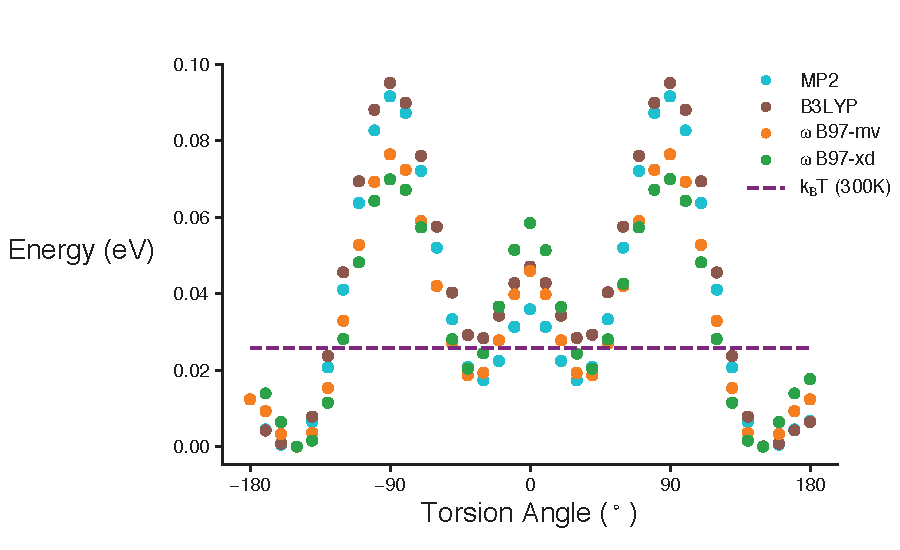
\includegraphics{figures/append_tor_model/SI_compare_theory_torsion.pdf}
    \caption[Ground-state PT Torsion Potential at Different Levels of Theory]{PT Ground-state torsion potential at different levels of theory. MP2 basis set: cc-pVTZ, B3LYP and $\omega$B97-xd basis set: 6-31++G**, $\omega$B97-mv basis set: def2-QZVPPD}
    \label{fig:gs_theory}
\end{figure}

\subsection{The Effect of Chain Length on Ground-state Torsion Angles}
\label{subsec:chain_length_gs}

Different polythiophene (PT) chain lengths were optimized at the RI-MP2 level (Table~\ref{tab:gs_RIMP2}). In all instances the optimized structures had non-planar central torsion angles corresponding to minima observed in Figure \ref{fig:gs_theory}. Additionally, the energy of optimized planar (trans) configurations were higher than that of optimized non-planar configurations. This evidence supports DuBay et al. in their claim that the torsion potential of conjugated polymers such as PT can be approximated by the dimer torsion potential if an appropriate level of theory, basis set, and optimization procedure are used \cite{Dubay2012}.

\begin{table}[hbt!]\centering
\caption{Ground-state Optimized Geometries}
\label{tab:gs_RIMP2}
\renewcommand{\arraystretch}{1.5}
\begin{threeparttable}
\begin{tabular}{cccc}\toprule
\multicolumn{1}{c}{\multirow{2}{2.5cm}{\centering Number of \\ Monomers}} &
\multicolumn{1}{c}{\multirow{2}{4.1cm}{\centering Trans Geometry \\ Abs. Energy (Hartree)}} &
\multicolumn{1}{c}{\multirow{2}{4.1cm}{\centering Optimized Geometry \\ Abs. Energy (Hartree)}} &
\multicolumn{1}{c}{\multirow{2}{4.1cm}{\centering Optimized Central  \\ Torsion Angle ($^\circ$)}} \\ \\ \midrule
    2 & -1103.35246329362\tnote{a} & -1103.35284395916\tnote{a} & 22\\
    4 & -2205.26456300358\tnote{b} & -2205.26519616574\tnote{b} & 161\\
    8 & -- & -4409.36496730408\tnote{b} & 159\\ \bottomrule
\end{tabular}
\begin{tablenotes}
\item[a] \footnotesize Theory: RI-MP2 basis set: cc-pVQZ
\item[b] \footnotesize Theroy: RI-MP2 basis set: cc-pVTZ
\end{tablenotes}
\end{threeparttable}
\end{table}


\subsection{The Effect of Chain Length on Doped Torsion Potentials}
\label{subsec:chain_length_cat}

The impact of chain length was investigated for doped torsion potentials to address concerns about charge and spin localization. In the end, the dimer approximation was suitable as it was in the ground state. The relaxation procedure detailed in the main text was altered for doped chains longer than $n = 4$ due to the polaron shifting away from the central torsion of interest for non-planar configurations. Shifting of the polaron can be seen in Figs.~\ref{fig:n6_bl} and \ref{fig:n8_bl} where the bond length distortion moves from the center to one of edges, while the $N = 2$ and $N = 4$ chains were too short for the polaron to have anywhere to shift (Figs. \ref{fig:n2_bl} and \ref{fig:n4_bl}). The modified relaxation procedure for the $N = 6$ and $N = 8$ doped chains consisted of an initial geometry optimization followed by single point energy calculations at each torsional configuration. This procedure maintained the position of the polaron on the central torsion angle of interest.

\begin{figure}[hbt!]
    \centering
    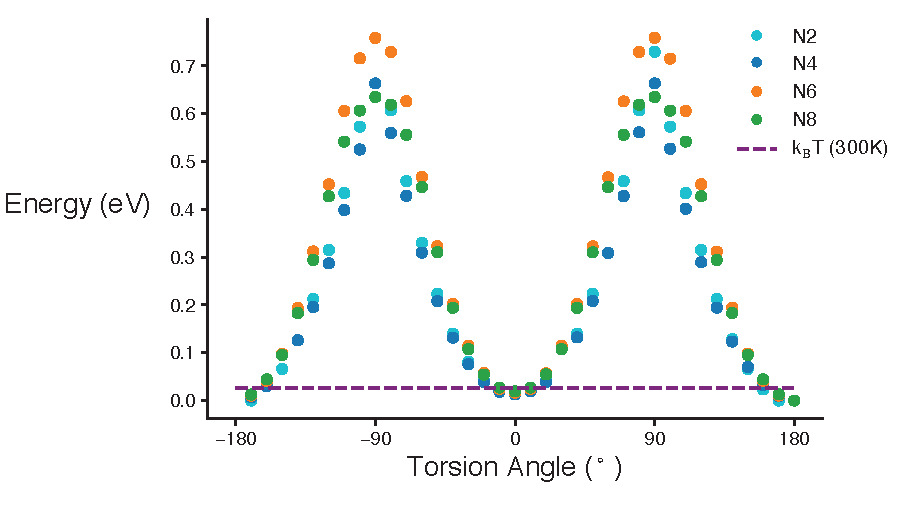
\includegraphics{figures/append_tor_model/SI_cat_diff_lens.pdf}
    \caption[Doped PT Torsion Potential for Different Chain Lengths]{Doped (cation) torsion potential for different chain lengths (N monomers). Functional: $\omega$B97-xd basis set: 6-31++G** }
    \label{fig:cat_dl}
\end{figure}

\begin{figure}[hbt!]
    \centering
    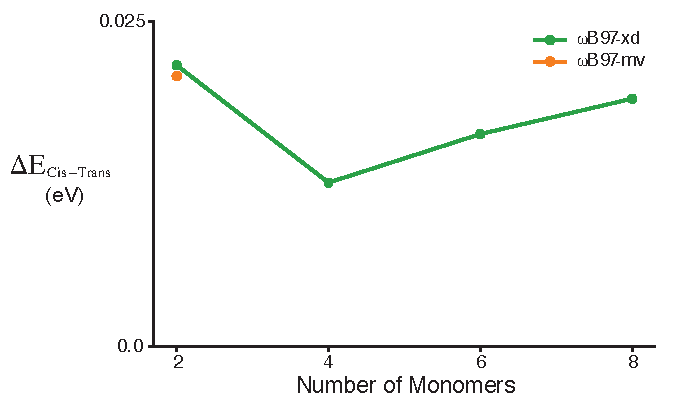
\includegraphics{figures/append_tor_model/delta_e_plot.pdf}
    \caption[Relative Energy Between PT Cis and Trans Configurations at Different Chain Lengths]{The relative energy between cis and trans configurations at different chain lengths.}
    \label{fig:delta_e}
\end{figure}

\clearpage
\begin{table}[hbt!]\centering
\captionsetup{justification=centering}
\captionsetup{width=.6\textwidth}
\captionsetup{skip=2pt}
\caption{Relative Energy Differences Between the Cis and the Trans Ground-state Configurations}
\renewcommand{\arraystretch}{1.5}
\begin{threeparttable}
\begin{tabular}{cccc}\toprule
  {Number of Monomers} & {$\Delta E_{ \ Cis - Trans}$ (eV)} \\ \midrule
    2 & 0.02079\tnote{a}\\
    2 & 0.02162\tnote{b}\\
    4 & 0.01260\tnote{b}\\
    6 & 0.01633\tnote{b}\\
    8 & 0.01905\tnote{b}\\ \bottomrule
\end{tabular}
\begin{tablenotes}
\item[a] \footnotesize Functional: $\omega$B97-mv basis set: def2-QZVPPD
\item[b] \footnotesize Functional: $\omega$B97-xd basis set: 6-31++G**
\end{tablenotes}
\end{threeparttable}
\end{table}

\begin{figure}[hbt!]
    \centering
    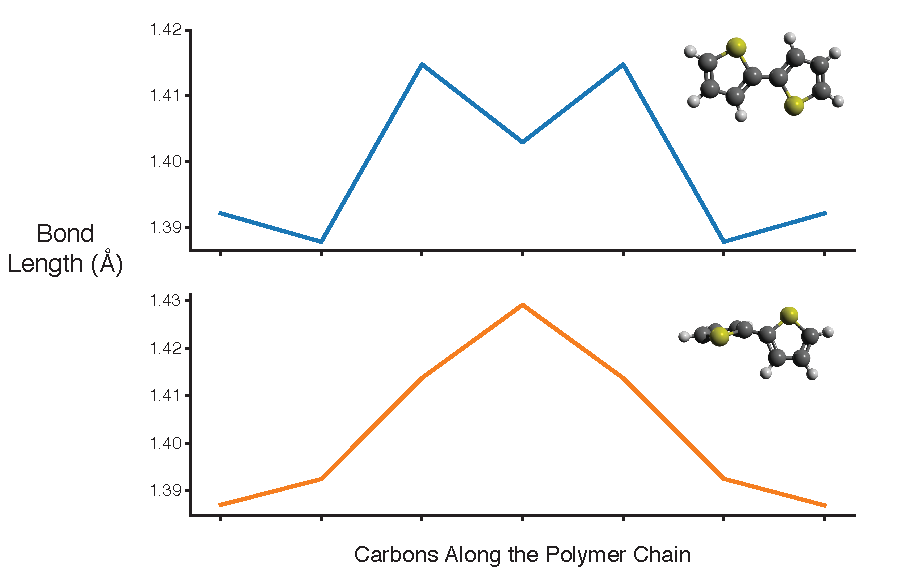
\includegraphics{figures/append_tor_model/n2_fig_w.pdf}
    \caption[Polaron Localization in PT Chain (N = 2)]{Carbon-Carbon bond lengths along the doped (cation) dimer. Top: Relaxed planar configuration, Bottom: Relaxed twisted configuration}
    \label{fig:n2_bl}
\end{figure}

\begin{figure}[hbt!]
    \centering
    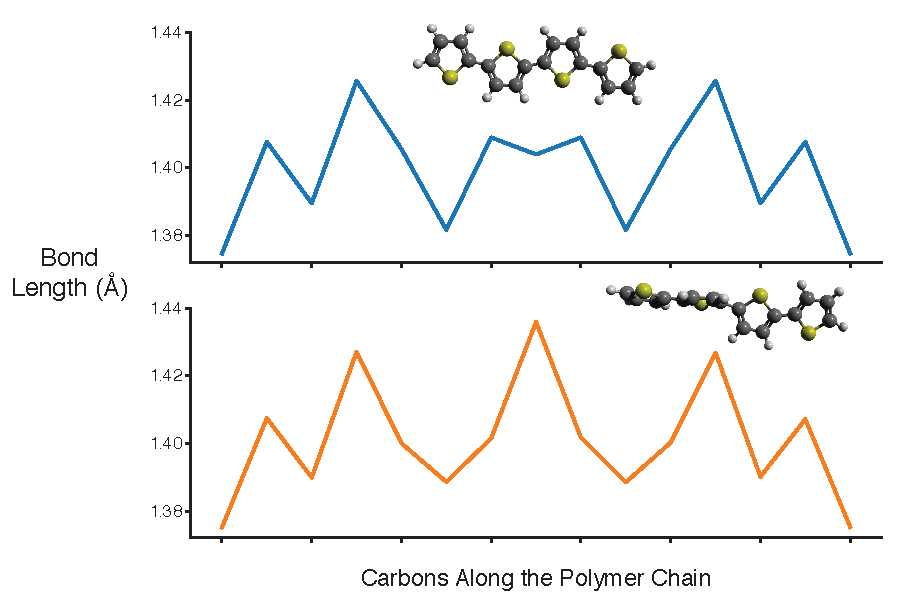
\includegraphics{figures/append_tor_model/n4_fig_w.pdf}
    \caption[Polaron Localization in PT Chain (N = 4)]{Carbon-Carbon bond lengths along the doped (cation) $N = 4$ chain. Top: Relaxed planar configuration, Bottom: Relaxed twisted configuration}
    \label{fig:n4_bl}
\end{figure}

\begin{figure}[hbt!]
    \centering
    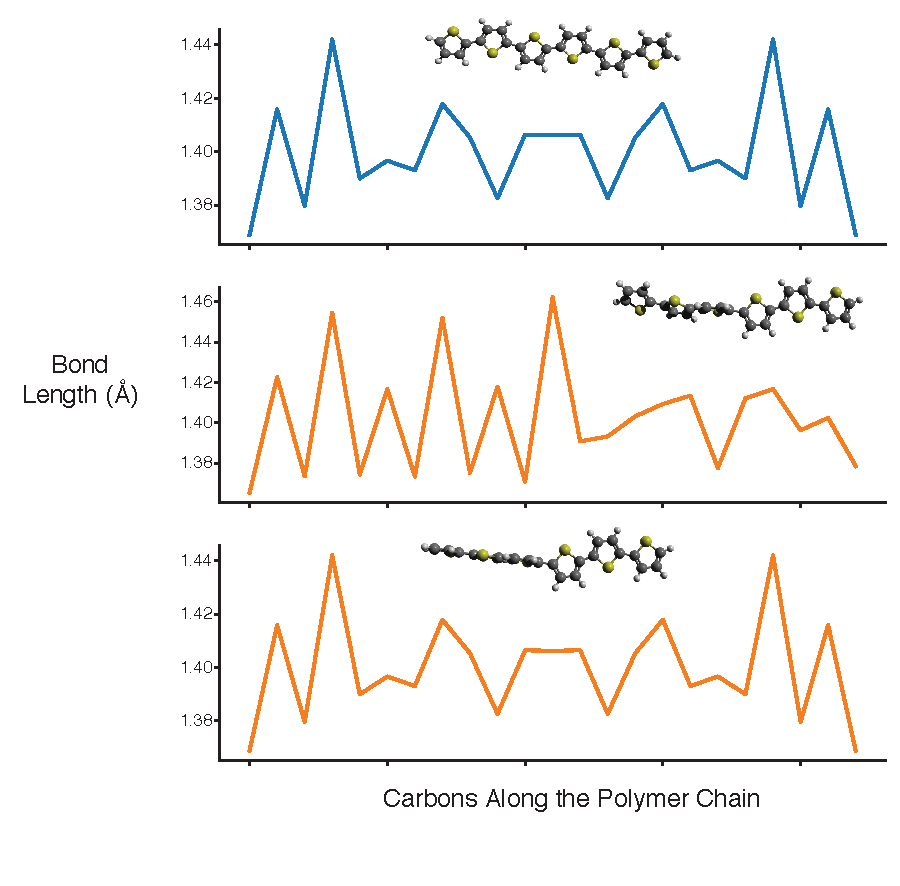
\includegraphics{figures/append_tor_model/n6_fig_w.pdf}
    \caption[Polaron Localization in PT Chain (N = 6)]{Carbon-Carbon bond lengths along the doped (cation) $N = 6$ chain. Top: Relaxed planar configuration, Middle: Relaxed twisted configuration, Bottom: Frozen twisted configuration}
    \label{fig:n6_bl}
\end{figure}

\begin{figure}[hbt!]
    \centering
    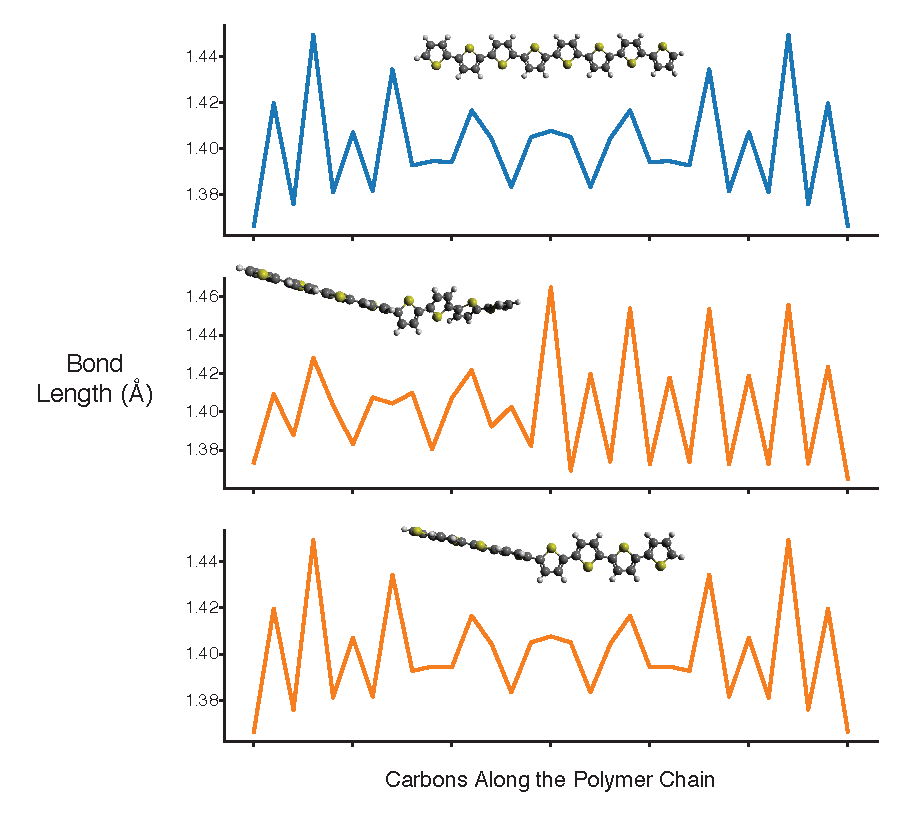
\includegraphics{figures/append_tor_model/n8_fig_w.pdf}
    \caption[Polaron Localization in PT Chain (N = 8)]{Carbon-Carbon bond lengths along the doped (cation) $N = 8$ chain. Top: Relaxed planar configuration, Middle: Relaxed twisted configuration, Bottom: Frozen twisted configuration}
    \label{fig:n8_bl}
\end{figure}

\clearpage

\subsection{Excited Torsion Potentials at Different Levels of Theory}

Previous work on organic conjugated molecules demonstrated that RO-DFT and UO-DFT were better than TDDFT at reproducing experimental electronic properties for the first triplet state (T1) \cite{Hait2016}. Nevertheless, TDDFT, RO-DFT, and UO-DFT were compared in table \ref{tab:ex_ct_gap} to understand the magnitude of energy differences between the theories.

\begin{table}[hbt!]\centering
\captionsetup{justification=centering}
\captionsetup{width=.6\textwidth}
\captionsetup{skip=2pt}
\caption{Relative Energy Differences Between the Cis and the Trans Excited (T1) Configurations}
\label{tab:ex_ct_gap}
\renewcommand{\arraystretch}{1.5}
\begin{threeparttable}
\begin{tabular}{cccc}\toprule
\multicolumn{1}{c}{\multirow{1}{3.5cm}{\centering }} &
\multicolumn{1}{c}{\multirow{1}{3.5cm}{\centering $\Delta E_{\ Cis - Trans}$ (eV)}} \\ \midrule
    TDDFT\tnote{\textdagger} & 0.02137\\
    UO-DFT\tnote{\textdagger} & 0.01338\\
    UO-DFT\tnote{*} & 0.01269\\
    RO-DFT\tnote{*} & 0.01609\\ \bottomrule
\end{tabular}
\begin{tablenotes}
\item[\textdagger] \footnotesize Functional: $\omega$B97-xd basis set: 6-31++G**
\item[*] \footnotesize Functional: $\omega$B97-mv basis set: def2-TZVPPD
\end{tablenotes}
\end{threeparttable}
\end{table}

\section{Polypyrrole Torsion Potentials}
\label{sec:ppy}
\subsection{Torsion Potential Comparison}

\begin{figure}[hbt!]
    \centering
    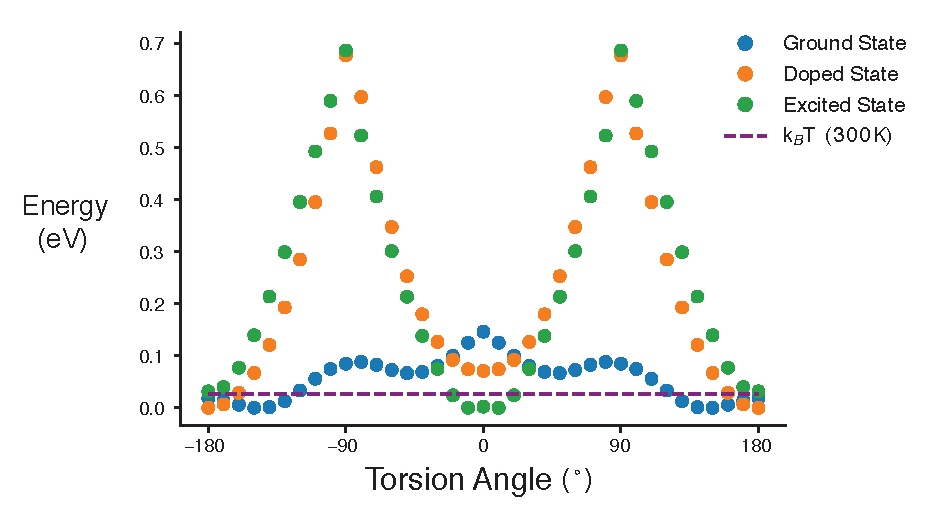
\includegraphics{figures/append_tor_model/ppy_torsion_compare.pdf}
    \caption[Comparison of the Ground, Doped, and Excited-state Torsion Potentials of PPy]{A comparison of the ground, doped (cation), and excited-state (first triplet) torsion potentials of pyrrole dimer molecules. Functional: $\omega$B97-mv basis set: def2-TZVPPD}
    \label{fig:ppy_tor}
\end{figure}

The pyrrole torsion potentials were assumed to be symmetric (i.e. only calculating the positive half of the potential) as they were with thiophene (See Subsection \ref{sec:TPF}\ref{subsec:TPF_descript}). We note that all the excited-state configurations had out-of-plane N-H hydrogens, whereas the doped-state configurations had all in-plane N-H hydrogens.

\clearpage

\subsection{Torsion Potential Data and Initial Structures}
\begin{table}[hbt!]\centering
\caption{Ground-state Pyrrole Dimer Initial Structure}
\renewcommand{\arraystretch}{1.5}
\begin{threeparttable}
\begin{tabular}{ccccc}\toprule
{} & {Atom} & {X (\AA)} & {Y (\AA)} & {Z (\AA)} \\ \midrule
    1  & N &  0.1438107 & -0.0411429 & -0.4535532\\
    2  & C &  1.4773229 & -0.0788175 & -0.1493554\\
    3  & H &  1.8151739 & -0.1383387 &  0.8700846\\
    4  & C &  2.1764672 & -0.0299186 & -1.3248901\\
    5  & H &  3.2487461 & -0.0316715 & -1.4199869\\
    6  & C &  1.2270605 &  0.0405707 & -2.3794193\\
    7  & H &  1.4372125 &  0.1342226 & -3.4320510\\
    8  & C & -0.0250831 &  0.0289564 & -1.8102511\\
    9  & C & -1.3498064 &  0.0805442 & -2.4043013\\
    10 & C & -2.5284819 &  0.6262933 & -1.9518871\\
    11 & H & -2.6535219 &  1.1765257 & -1.0340344\\
    12 & C & -3.5191498 &  0.3838374 & -2.9409496\\
    13 & H & -4.5519255 &  0.6856820 & -2.9082884\\
    14 & C & -2.9158139 & -0.2956872 & -3.9643888\\
    15 & H & -3.3097283 & -0.6661324 & -4.8941293\\
    16 & N & -1.6006395 & -0.4734122 & -3.6306845\\
    17 & H & -0.6104249 & -0.1240319 &  0.2028327\\
    18 & H & -0.9253188 & -0.9915794 & -4.1617169\\ \bottomrule
\end{tabular}
\begin{tablenotes}
\item[*] \footnotesize Atomic coordinates are reported to the full quantum chemistry software precision for reproducibility purposes, although they do not reflect the true number of significant digits.
\end{tablenotes}
\end{threeparttable}
\end{table}

\begin{table}[hbt!]\centering
\caption{Ground-state Pyrrole Dimer Torsion Data}
\renewcommand{\arraystretch}{1.5}
\begin{threeparttable}
\begin{tabular}{cccc}\toprule
  {} & {Torsion Angle} & {Rel. Energy (eV)} & {Abs. Energy (Hartree)} \\ \midrule
    1  & 0.0   & 0.14631 & -419.150251034421\\
    2  & 10.0  & 0.12506 & -419.151031655173\\
    3  & 20.0  & 0.09972 & -419.151963159215\\
    4  & 30.0  & 0.08050 & -419.152669398895\\
    5  & 40.0  & 0.06897 & -419.153092977519\\
    6  & 50.0  & 0.06674 & -419.153175077438\\
    7  & 60.0  & 0.07273 & -419.152954901242\\
    8  & 70.0  & 0.08265 & -419.152590252506\\
    9  & 80.0  & 0.08828 & -419.152383572136\\
    10 & 90.0  & 0.08456 & -419.152520200073\\
    11 & 100.0 & 0.07462 & -419.152885388511\\
    12 & 110.0 & 0.05579 & -419.153577293422\\
    13 & 120.0 & 0.03306 & -419.154412807997\\
    14 & 130.0 & 0.01279 & -419.155157674912\\
    15 & 140.0 & 0.00121 & -419.155583069180\\
    16 & 150.0 & 0.00000 & -419.155627663140\\
    17 & 160.0 & 0.00582 & -419.155413621542\\
    18 & 170.0 & 0.01394 & -419.155115472566\\
    19 & 180.0 & 0.01848 & -419.154948650234\\ \bottomrule
\end{tabular}
\begin{tablenotes}
\item[*] \footnotesize Energy values are reported to the full quantum chemistry software precision for reproducibility purposes, although they do not reflect the true number of significant digits.
\end{tablenotes}
\end{threeparttable}
\end{table}

\begin{table}[hbt!]\centering
\caption{Doped-state Pyrrole Dimer Initial Structure}
\renewcommand{\arraystretch}{1.5}
\begin{threeparttable}
\begin{tabular}{ccccc}\toprule
{} & {Atom} & {X (\AA)} & {Y (\AA)} & {Z (\AA)} \\ \midrule
    1  & N &  0.1244013 & -0.0124993 & -0.4386263\\
    2  & C &  1.4375902 & -0.0551168 & -0.1587828\\
    3  & H &  1.7929559 & -0.0891701 &  0.8573685\\
    4  & C &  2.1557384 & -0.0461157 & -1.3603672\\
    5  & H &  3.2278057 & -0.0736121 & -1.4461102\\
    6  & C &  1.2344603 &  0.0037460 & -2.3853068\\
    7  & H &  1.4529189 &  0.0231124 & -3.4400252\\
    8  & C & -0.0592961 &  0.0253156 & -1.8067791\\
    9  & C & -1.3176295 &  0.0746973 & -2.4037290\\
    10 & C & -2.6113886 &  0.0961671 & -1.8252036\\
    11 & H & -2.8298491 &  0.0767245 & -0.7704869\\
    12 & C & -3.5326670 &  0.1460190 & -2.8501433\\
    13 & H & -4.6047365 &  0.1734334 & -2.7644022\\
    14 & C & -2.8145161 &  0.1551214 & -4.0517254\\
    15 & H & -3.1698811 &  0.1892087 & -5.0678758\\
    16 & N & -1.5013265 &  0.1125333 & -3.7718813\\
    17 & H & -0.6094801 & -0.0090223 &  0.2491140\\
    18 & H & -0.7674401 &  0.1092375 & -4.4596173\\ \bottomrule
\end{tabular}
\begin{tablenotes}
\item[*] \footnotesize Atomic coordinates are reported to the full quantum chemistry software precision for reproducibility purposes, although they do not reflect the true number of significant digits.
\end{tablenotes}
\end{threeparttable}
\end{table}

\begin{table}[hbt!]\centering
\caption{Doped-state Pyrrole Dimer Torsion Data}
\renewcommand{\arraystretch}{1.5}
\begin{threeparttable}
\begin{tabular}{cccc}\toprule
  {} & {Torsion Angle} & {Rel. Energy (eV)} & {Abs. Energy (Hartree)} \\ \midrule
    1  & 0.0   & 0.07089 & -418.901257453274\\
    2  & 10.0  & 0.07429 & -418.901132469421\\
    3  & 20.0  & 0.09209 & -418.900478404582\\
    4  & 30.0  & 0.12671 & -418.899206193558\\
    5  & 40.0  & 0.17981 & -418.897254678549\\
    6  & 50.0  & 0.25308 & -418.894562034780\\
    7  & 60.0  & 0.34742 & -418.891095239250\\
    8  & 70.0  & 0.46244 & -418.886868205963\\
    9  & 80.0  & 0.59734 & -418.881910697353\\
    10 & 90.0  & 0.67736 & -418.878970154026\\
    11 & 100.0 & 0.52725 & -418.884486309677\\
    12 & 110.0 & 0.39525 & -418.889337414907\\
    13 & 120.0 & 0.28493 & -418.893391476576\\
    14 & 130.0 & 0.19303 & -418.896768641865\\
    15 & 140.0 & 0.12081 & -418.899422743259\\
    16 & 150.0 & 0.06695 & -418.901402028751\\
    17 & 160.0 & 0.02869 & -418.902808261839\\
    18 & 170.0 & 0.00670 & -418.903616153827\\
    19 & 180.0 & 0.00000 & -418.903862534217\\ \bottomrule
\end{tabular}
\begin{tablenotes}
\item[*] \footnotesize Energy values are reported to the full quantum chemistry software precision for reproducibility purposes, although they do not reflect the true number of significant digits.
\end{tablenotes}
\end{threeparttable}
\end{table}

\begin{table}[hbt!]\centering
\caption{Excited-state Pyrrole Dimer Initial Structure}
\renewcommand{\arraystretch}{1.5}
\begin{threeparttable}
\begin{tabular}{ccccc}\toprule
{} & {Atom} & {X (\AA)} & {Y (\AA)} & {Z (\AA)} \\ \midrule
    1  & N &  0.1182567 & -0.0133505 & -0.4140073\\
    2  & C &  1.4646611 & -0.0561109 & -0.1446613\\
    3  & H &  1.8347408 & -0.0900216 &  0.8645974\\
    4  & C &  2.1636990 & -0.0465331 & -1.3510586\\
    5  & H &  3.2374443 & -0.0739927 & -1.4346225\\
    6  & C &  1.2593069 &  0.0028204 & -2.3920959\\
    7  & H &  1.4835638 &  0.0218852 & -3.4447711\\
    8  & C & -0.0840740 &  0.0257577 & -1.8116935\\
    9  & C & -1.2928575 &  0.0740333 & -2.3988200\\
    10 & C & -2.6362423 &  0.0968297 & -1.8184208\\
    11 & H & -2.8605020 &  0.0776395 & -0.7657483\\
    12 & C & -3.5406287 &  0.1463965 & -2.8594527\\
    13 & H & -4.6143750 &  0.1738185 & -2.7758897\\
    14 & C & -2.8415852 &  0.1561874 & -4.0658453\\
    15 & H & -3.2116588 &  0.1903313 & -5.0750983\\
    16 & N & -1.4951883 &  0.1131461 & -3.7965062\\
    17 & H & -0.6132396 & -0.0095123 &  0.2682338\\
    18 & H & -0.7636611 &  0.1104555 & -4.4787197\\ \bottomrule
\end{tabular}
\begin{tablenotes}
\item[*] \footnotesize Atomic coordinates are reported to the full quantum chemistry software precision for reproducibility purposes, although they do not reflect the true number of significant digits.
\end{tablenotes}
\end{threeparttable}
\end{table}

\begin{table}[hbt!]\centering
\caption{Excited-state Pyrrole Dimer Torsion Data}
\renewcommand{\arraystretch}{1.5}
\begin{threeparttable}
\begin{tabular}{cccc}\toprule
  {} & {Torsion Angle} & {Rel. Energy (eV)} & {Abs. Energy (Hartree)} \\ \midrule
    1  & 0.0   & 0.00220 & -419.046809351616\\
    2  & 10.0  & 0.00000 & -419.046890120689\\
    3  & 20.0  & 0.02409 & -419.046004873362\\
    4  & 30.0  & 0.07461 & -419.044148392034\\
    5  & 40.0  & 0.13811 & -419.041814659066\\
    6  & 50.0  & 0.21347 & -419.039045122861\\
    7  & 60.0  & 0.30119 & -419.035821446878\\
    8  & 70.0  & 0.40608 & -419.031967123697\\
    9  & 80.0  & 0.52308 & -419.027667141569\\
    10 & 90.0  & 0.68681 & -419.021650431473\\
    11 & 100.0 & 0.58994 & -419.025210117559\\
    12 & 110.0 & 0.49281 & -419.028779613372\\
    13 & 120.0 & 0.39563 & -419.032351154440\\
    14 & 130.0 & 0.29921 & -419.035894226825\\
    15 & 140.0 & 0.21374 & -419.039035324061\\
    16 & 150.0 & 0.13956 & -419.041761426001\\
    17 & 160.0 & 0.07696 & -419.044061759566\\
    18 & 170.0 & 0.03992 & -419.045423017008\\
    19 & 180.0 & 0.03172 & -419.045724381281\\ \bottomrule
\end{tabular}
\begin{tablenotes}
\item[*] \footnotesize Energy values are reported to the full quantum chemistry software precision for reproducibility purposes, although they do not reflect the true number of significant digits.
\end{tablenotes}
\end{threeparttable}
\end{table}

\clearpage

\section{Torsion Potential Fitting}
\label{sec:TPF}
\subsection{Description}
\label{subsec:TPF_descript}
Thiophene torsion potentials were assumed to be symmetric because of the symmetry displayed in the dimer unit. As a result, only half of the torsion potential (0-180\textdegree) was calculated. The full range (-180-180\textdegree) of data points were fitted with the Ryckaert-Bellemans (RB) function (eq 1). In all cases a non-linear least squares method was used to fit the RB function (scipy.optimize.curve\_fit) \cite{Jones}. The ground-state torsion potential used a weighted fit where torsion angle minima and maxima points (-180\textdegree, -150\textdegree, -40\textdegree, 180\textdegree, 150\textdegree, 40\textdegree) were weighted by a factor of 50 and 0\textdegree\ by a factor of 100. The weights were chosen to find a balance between the total sum of the squared residuals (SSR) and the SSR of data points whose energies fell below the relevant energy scale (2$k_B$T where T=300K). Additional weight was placed on the 0\textdegree\ torsion angle because of its importance on chain structure in PT. The doped and excited torsion potentials were fit using Boltzmann weights (T=300K). For visualization purposes only, the doped and excited potentials (i.e. fig. 1) were fit by weighting the torsion angles with energies below (2$k_B$T where T=300K) by a factor of 100 and 0\textdegree\ a factor of 500. The fitting values used in numerical simulations can be found below.

\subsection{Fitting Parameters}
\begin{table}[hbt!]\centering
\caption{Ryckaert-Bellemans Coefficients}
\renewcommand{\arraystretch}{1.5}
\begin{threeparttable}
\begin{tabular}{ccccccc}\toprule
\multicolumn{1}{c}{\multirow{1}{3.5cm}{\centering}} &
\multicolumn{1}{c}{\multirow{1}{1.5cm}{\centering c0}} &
\multicolumn{1}{c}{\multirow{1}{1.5cm}{\centering c1}} &
\multicolumn{1}{c}{\multirow{1}{1.5cm}{\centering c2}} &
\multicolumn{1}{c}{\multirow{1}{1.5cm}{\centering c3}} &
\multicolumn{1}{c}{\multirow{1}{1.5cm}{\centering c4}} &
\multicolumn{1}{c}{\multirow{1}{1.5cm}{\centering c5}} \\ \midrule
    Ground State\tnote{\textdagger} & 0.0781 & 0.009154 & -0.2098 & -0.0038 & 0.1608 & 0.0114\\
    Doped State\tnote{*} & 0.4421 & 0.0329 & -0.5769 & -0.0868 & 0.1453 & 0.0642\\
    Excited State\tnote{*} & 0.6336 & 0.0718 & -0.7751 & -0.1993 & 0.1478 & 0.1338\\ \bottomrule
\end{tabular}
\begin{tablenotes}
\item[\textdagger] \footnotesize Minima and Maxima Weighted Fit
\item[*] \footnotesize Boltzmann Weighted Fit
\end{tablenotes}
\end{threeparttable}
\end{table}

\section{Torsion Potential Model}
\label{sec:TPM}
\subsection{Description}
To reduce computational burden and make the algorithm as general as possible atomistic chains were coarse grained into tangent lines connected by the appropriate bond lengths and bond angles. The coarse grain mapping for PT is shown in figure \ref{fig:cg_model}. As demonstrated in the main text figure \ref{fig:comp_tor}, the central bond length changes for the doped and excited chains. Additionally, bond angles change in the doped and excited chains. These changes were accounted for in the model, and the values used can be found in table \ref{tab:tpm_vals}. Tangent lengths and bond lengths were taken from the initially optimized structures whereas the bond angles were taken as the Boltzmann weighted average across all torsion angle configurations optimized with quantum chemistry.

\begin{figure}[hbt!]
    \centering
    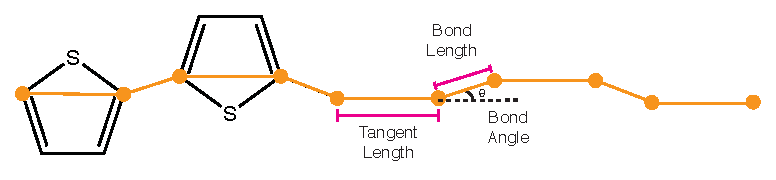
\includegraphics{figures/append_tor_model/course_grain_model.pdf}
    \caption[Coarse Grained Mapping for PT]{The coarse grained mapping for polythiophene. The tangent length, bond length, and bond angle are general inputs for the torsion potential model}
    \label{fig:cg_model}
\end{figure}

\begin{table}[hbt!]\centering
\caption{Torsion Potential Model Values}
\label{tab:tpm_vals}
\renewcommand{\arraystretch}{1.5}
\begin{threeparttable}
\begin{tabular}{cccc}\toprule
\multicolumn{1}{c}{\multirow{2}{3.5cm}{\centering }} &
\multicolumn{1}{c}{\multirow{2}{2.5cm}{\centering Tangent \\ Length (\AA)\tnote{\textdagger}}} &
\multicolumn{1}{c}{\multirow{2}{2.5cm}{\centering Bond \\ Length (\AA)\tnote{\textdagger}}} &
\multicolumn{1}{c}{\multirow{2}{2.5cm}{\centering Bond \\ Angle ($^\circ$)\tnote{*}}} \\ \\ \midrule
    Ground State & 2.47 & 1.46 & 15.2\\
    Doped State & 2.45 & 1.40 & 14.3\\
    Excited State & 2.50 & 1.35 & 14.1\\ \bottomrule
\end{tabular}
\begin{tablenotes}
\item[\textdagger] \footnotesize Taken from initial optimized geometry
\item[*] \footnotesize Boltzmann weighted average over all optimized torsion configurations
\end{tablenotes}
\end{threeparttable}
\end{table}

\subsection{Code}
The code used to generate chain conformations and collect chain statistics is freely available at \url{https://github.com/wood-b/dihedral_model}.

\section{Persistence Length \& End-to-end Distance}
\label{sec:lp}
\begin{equation}
\Large
\Big \langle \large \hat{\nu_i} \cdot \hat{\nu_{i+n}} \Big \rangle = \exp{\bigg(-\frac{n}{\chi l_{n}}\bigg)}
\label{eq:lN}
\end{equation}

\subsection{Tangent-tangent Correlation Function}

The tangent-tangent correlation function (Eq.~\ref{eq:lp}) can be rewritten into a form (Eq.~\ref{eq:lN}) that is easier to employ in practice by utilizing $L \approx m_ln$ and $l_p = m_ll_n$. The variable $l_n$ is the persistence length in monomer units ($n$). Additionally, the tangent-tangent correlation function can be normalized to decay from 1 by using unit backbone vectors ($\hat{\nu}$). Final $l_p$ values were computed by exponentially fitting the tangent-tangent correlation function \ref{eq:lN} and dimensionalizing $l_n$ using the relationship $l_p = m_ll_n$.

\subsection{Worm-like Chain Fitting}

End-to-end distances ($\sqrt{\big \langle R^2 \big \rangle}$) generated from the torsion potential model were compared with end-to-end distances from the 3D-WLC and the 2D-WLC (Figures \ref{fig:gs_wlc}, \ref{fig:d_wlc}, \ref{fig:e_wlc}). WLC end-to-end distances were calculated analytically using Eq.~\ref{eq:wlc_msqr}. Input $l_p$ values were computed from Eq.~\ref{eq:lN} using data from the torsion potential model and the appropriate $\chi$ value (i.e. $\chi = 1$ for 3D and $\chi = 2$ for 2D).

After comparing end-to-end distances of the WLC-3D, WLC-2D, and the torsion potential model it was clear that $l_p$ values for the torsion potential model could be improved by fitting $\chi$. $\chi$ values were determined by the ratio of the 3D-WLC $\big \langle R^2 \big \rangle$ and the torsion potential model $\big \langle R^2 \big \rangle$ at $N = 200$ for all values of $\alpha$ (Tables \ref{tab:d_lp} \ref{tab:e_lp}). In the end, $\chi$ values did not change that much over the range of $\alpha$ values. In the future, an average value of $\chi$ could be used.

\begin{equation}
\Large
\Big\langle R^2 \Big\rangle = 2l_p - 2l_p^2 \left(1 - e^{L/l_p} \right)
\label{eq:wlc_msqr}
\end{equation}

\begin{figure}[hbt!]
    \centering
    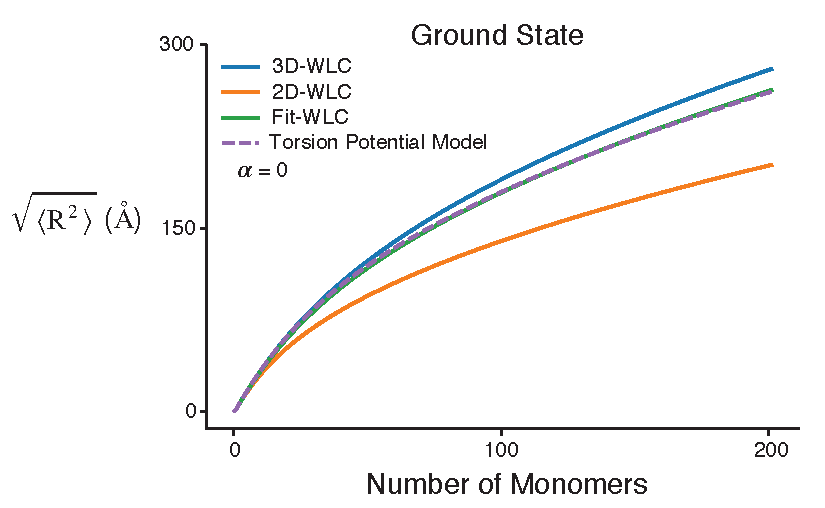
\includegraphics{figures/append_tor_model/gs_wlc_fit.pdf}
    \caption[Ground-state End-to-end Distance of the 2D-WLC, 3D-WLC, Torsion Potential Model, and Fit-WLC]{Ground-state end-to-end distances for the 2D and 3D WLC, the torsion potential model, and the WLC where $\chi$ was fit to torsion potential model.}
    \label{fig:gs_wlc}
\end{figure}

\begin{figure}[hbt!]
    \centering
    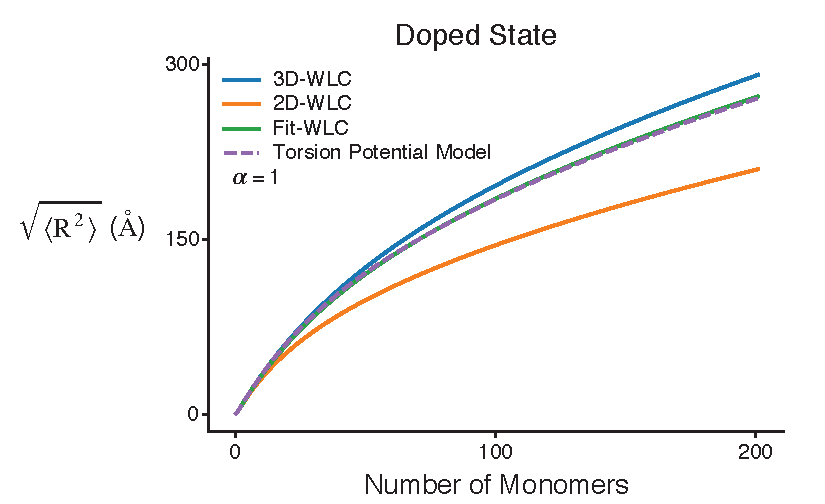
\includegraphics{figures/append_tor_model/cat_wlc_fit.pdf}
    \caption[Doped-state End-to-end Distance of the 2D-WLC, 3D-WLC, Torsion Potential Model, and Fit-WLC]{Doped-state end-to-end distances for the 2D and 3D WLC, the torsion potential model, and the WLC where $\chi$ was fit to torsion potential model.}
    \label{fig:d_wlc}
\end{figure}

\begin{figure}[hbt!]
    \centering
    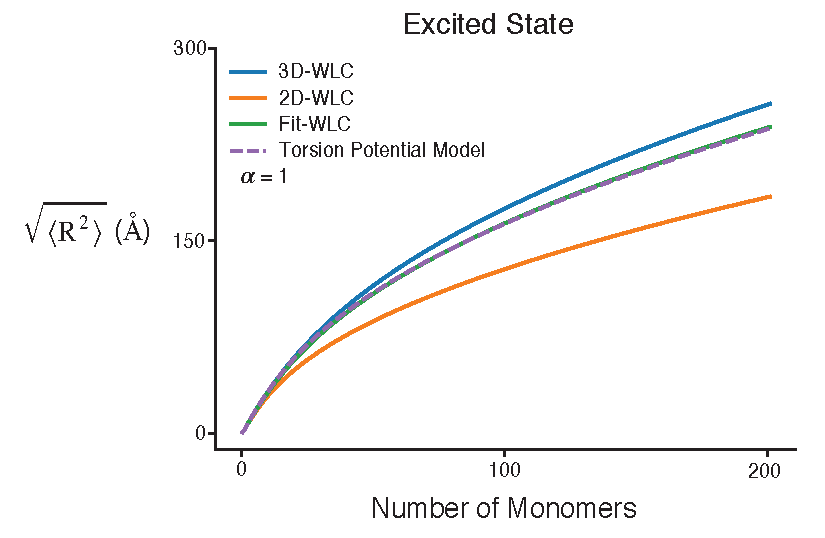
\includegraphics{figures/append_tor_model/trip_wlc_fit.pdf}
    \caption[Doped-state End-to-end Distance of the 2D-WLC, 3D-WLC, Torsion Potential Model, and Fit-WLC]{Excited-state end-to-end distances for the 2D and 3D WLC, the torsion potential model, and the WLC where $\chi$ was fit to torsion potential model.}
    \label{fig:e_wlc}
\end{figure}

\clearpage
\subsection{Persistence Length Data}
\begin{table}[hbt!]\centering
\caption{Doped Persistence Length Values}
\label{tab:d_lp}
\renewcommand{\arraystretch}{1.5}
\begin{threeparttable}
\begin{tabular}{ccccc}\toprule
\multicolumn{1}{c}{\multirow{1}{3.5cm}{\centering $\alpha$}} &
\multicolumn{1}{c}{\multirow{1}{1.5cm}{\centering $\chi$}} &
\multicolumn{1}{c}{\multirow{1}{1.5cm}{\centering $m_l$}} &
\multicolumn{1}{c}{\multirow{1}{1.5cm}{\centering $l_p$}} & \\ \midrule
    0.0 & 1.147 & 3.88 & 4.74\\
    0.05 & 1.146 & 3.88 & 4.75\\
    0.1 & 1.151 & 3.87 & 4.77\\
    0.15 & 1.147 & 3.87 & 4.81\\
    0.2 & 1.146 & 3.87 & 4.84\\
    0.25 & 1.153 & 3.86 & 4.84\\
    0.3 & 1.147 & 3.86 & 4.88\\
    0.35 & 1.148 & 3.86 & 4.91\\
    0.4 & 1.142 & 3.85 & 4.96\\
    0.45 & 1.156 & 3.85 & 4.90\\
    0.5 & 1.153 & 3.85 & 4.98\\
    0.55 & 1.146 & 3.84 & 5.03\\
    0.6 & 1.147 & 3.84 & 5.04\\
    0.65 & 1.149 & 3.83 & 5.08\\
    0.7 & 1.149 & 3.83 & 5.10\\
    0.75 & 1.152 & 3.83 & 5.13\\
    0.8 & 1.151 & 3.82 & 5.15\\
    0.85 & 1.149 & 3.82 & 5.18\\
    0.9 & 1.151 & 3.82 & 5.20\\
    0.95 & 1.148 & 3.81 & 5.24\\
    1.0 & 1.154 & 3.81 & 5.22\\ \bottomrule
\end{tabular}
\begin{tablenotes}
\item
\end{tablenotes}
\end{threeparttable}
\end{table}

\begin{table}[hbt!]\centering
\caption{Excited Persistence Length Values}
\label{tab:e_lp}
\renewcommand{\arraystretch}{1.5}
\begin{threeparttable}
\begin{tabular}{ccccc}\toprule
\multicolumn{1}{c}{\multirow{1}{3.5cm}{\centering $\alpha$}} &
\multicolumn{1}{c}{\multirow{1}{1.5cm}{\centering $\chi$}} &
\multicolumn{1}{c}{\multirow{1}{1.5cm}{\centering $m_l$}} &
\multicolumn{1}{c}{\multirow{1}{1.5cm}{\centering $l_p$}} & \\ \midrule
    0.0 & 1.147 & 3.88 & 4.74\\
    0.05 & 1.146 & 3.88 & 4.70\\
    0.1 & 1.148 & 3.87 & 4.65\\
    0.15 & 1.146 & 3.87 & 4.61\\
    0.2 & 1.151 & 3.87 & 4.56\\
    0.25 & 1.152 & 3.86 & 4.52\\
    0.3 & 1.149 & 3.86 & 4.50\\
    0.35 & 1.150 & 3.86 & 4.46\\
    0.4 & 1.150 & 3.85 & 4.42\\
    0.45 & 1.153 & 3.85 & 4.37\\
    0.5 & 1.155 & 3.85 & 4.32\\
    0.55 & 1.147 & 3.84 & 4.33\\
    0.6 & 1.154 & 3.84 & 4.27\\
    0.65 & 1.148 & 3.83 & 4.26\\
    0.7 & 1.149 & 3.83 & 4.21\\
    0.75 & 1.152 & 3.83 & 4.16\\
    0.8 & 1.153 & 3.82 & 4.13\\
    0.85 & 1.154 & 3.82 & 4.09\\
    0.9 & 1.153 & 3.82 & 4.07\\
    0.95 & 1.151 & 3.81 & 4.03\\
    1.0 & 1.168 & 3.81 & 3.93\\ \bottomrule
\end{tabular}
\begin{tablenotes}
\item
\end{tablenotes}
\end{threeparttable}
\end{table}

\clearpage
\subsection{Sampled Torsion Angle Distributions}

Torsion angle histograms at different values of $\alpha$ (Figure \ref{fig:a_0_hist}, \ref{fig:a_025_hist}, \ref{fig:a_050_hist}, \ref{fig:a_075_hist}, and \ref{fig:a_1_hist}) demonstrate that excited chains consistently contained more cis (0\textdegree) \ torsion angles, which ultimately resulted in the excited chains being shorter.

\begin{figure}[hbt!]
    \centering
    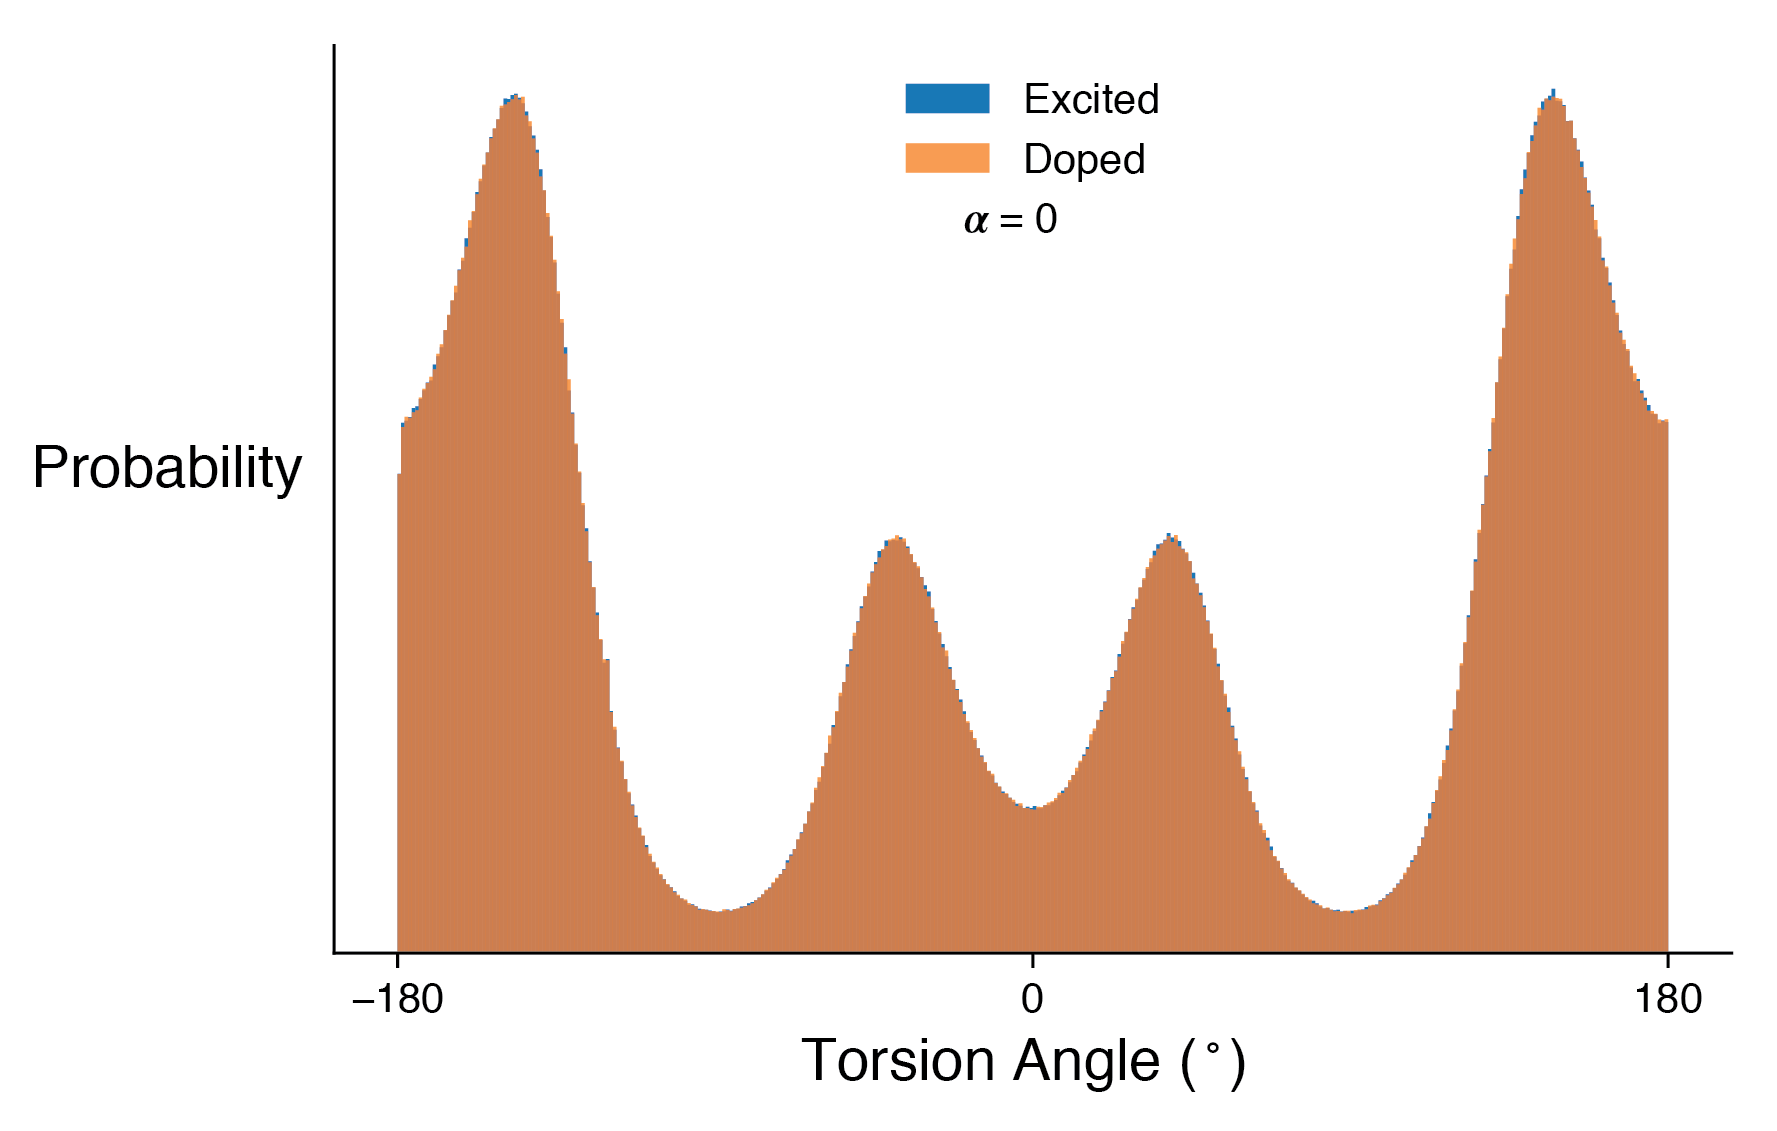
\includegraphics{figures/append_tor_model/a_0_hist.png}
    \caption[Histogram of Doped and Excited Sampled Torsion Angles at $\alpha = 0$]{Overlaid histograms of doped and excited sampled torsion angles at $\alpha = 0$}
    \label{fig:a_0_hist}
\end{figure}

\begin{figure}[hbt!]
    \centering
    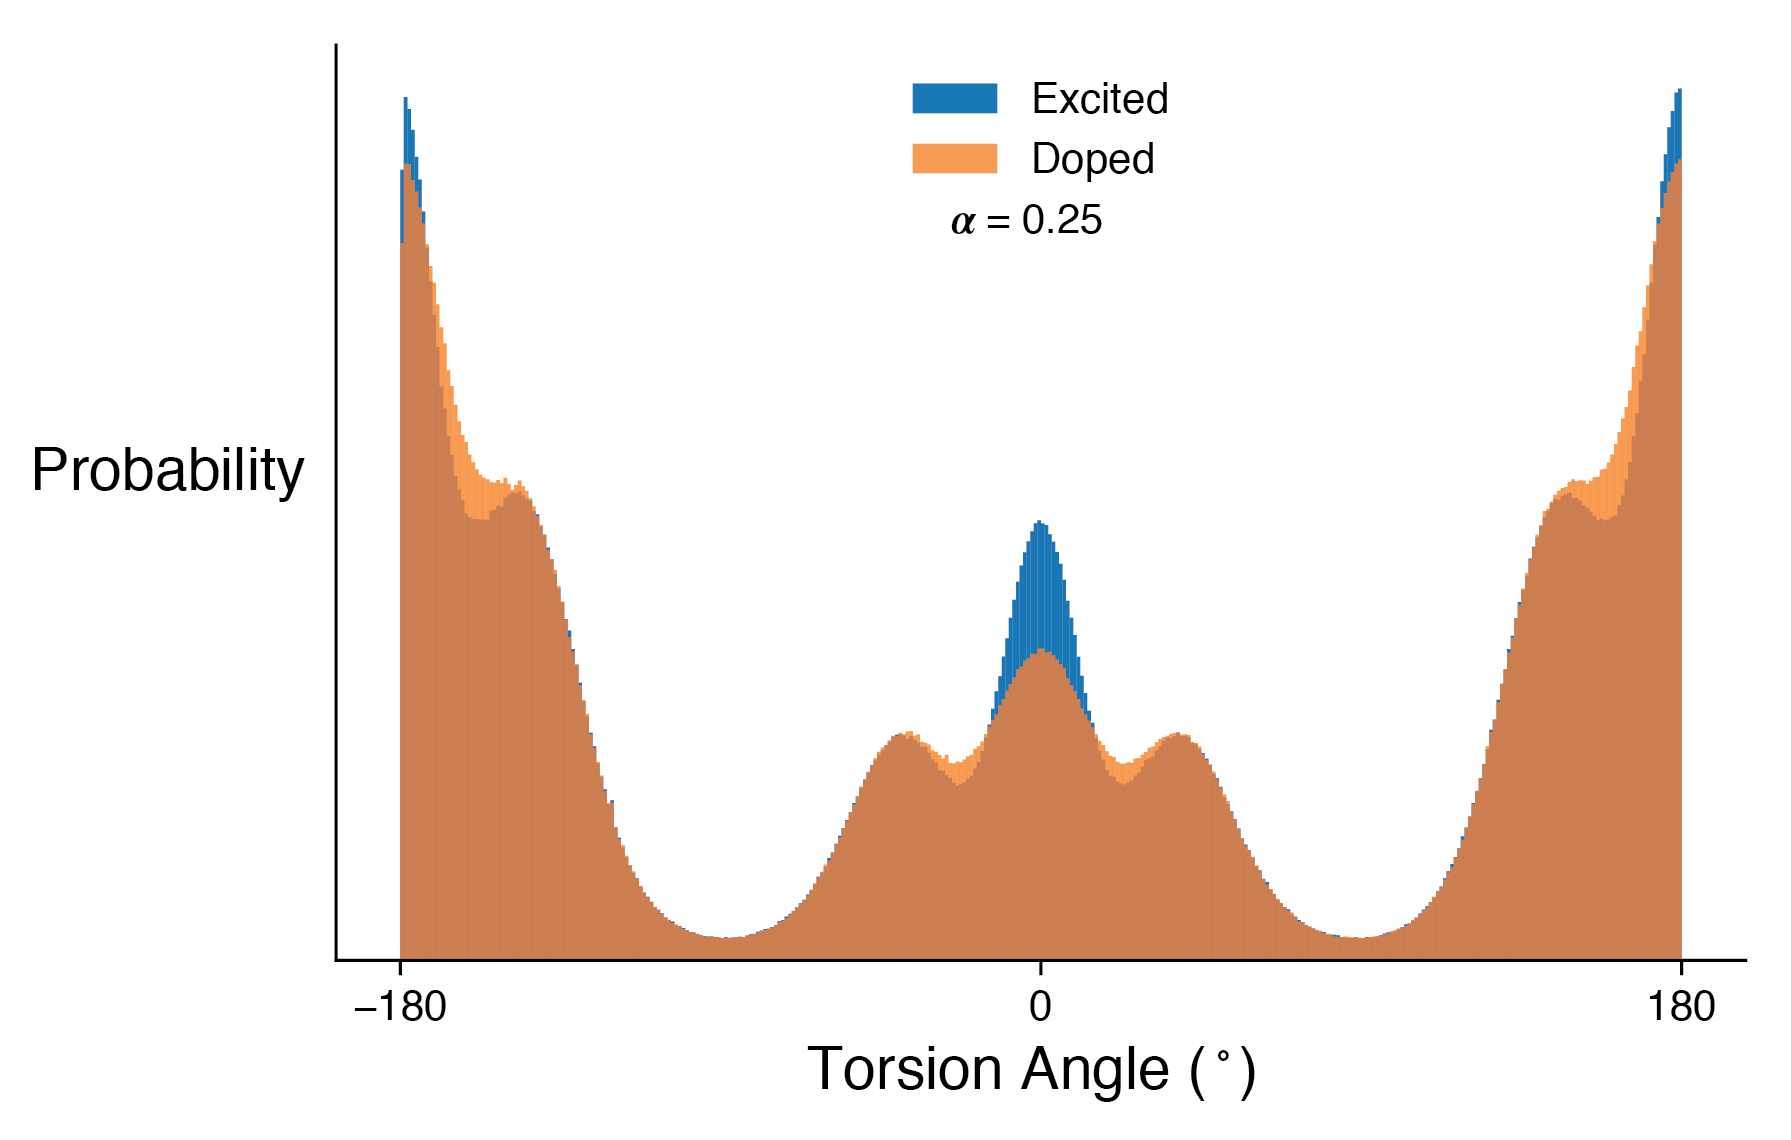
\includegraphics{figures/append_tor_model/a_025_hist.png}
    \caption[Histogram of Doped and Excited Sampled Torsion Angles at $\alpha = 0.25$]{Overlaid histograms of doped and excited sampled torsion angles at $\alpha = 0.25$}
    \label{fig:a_025_hist}
\end{figure}

\begin{figure}[hbt!]
    \centering
    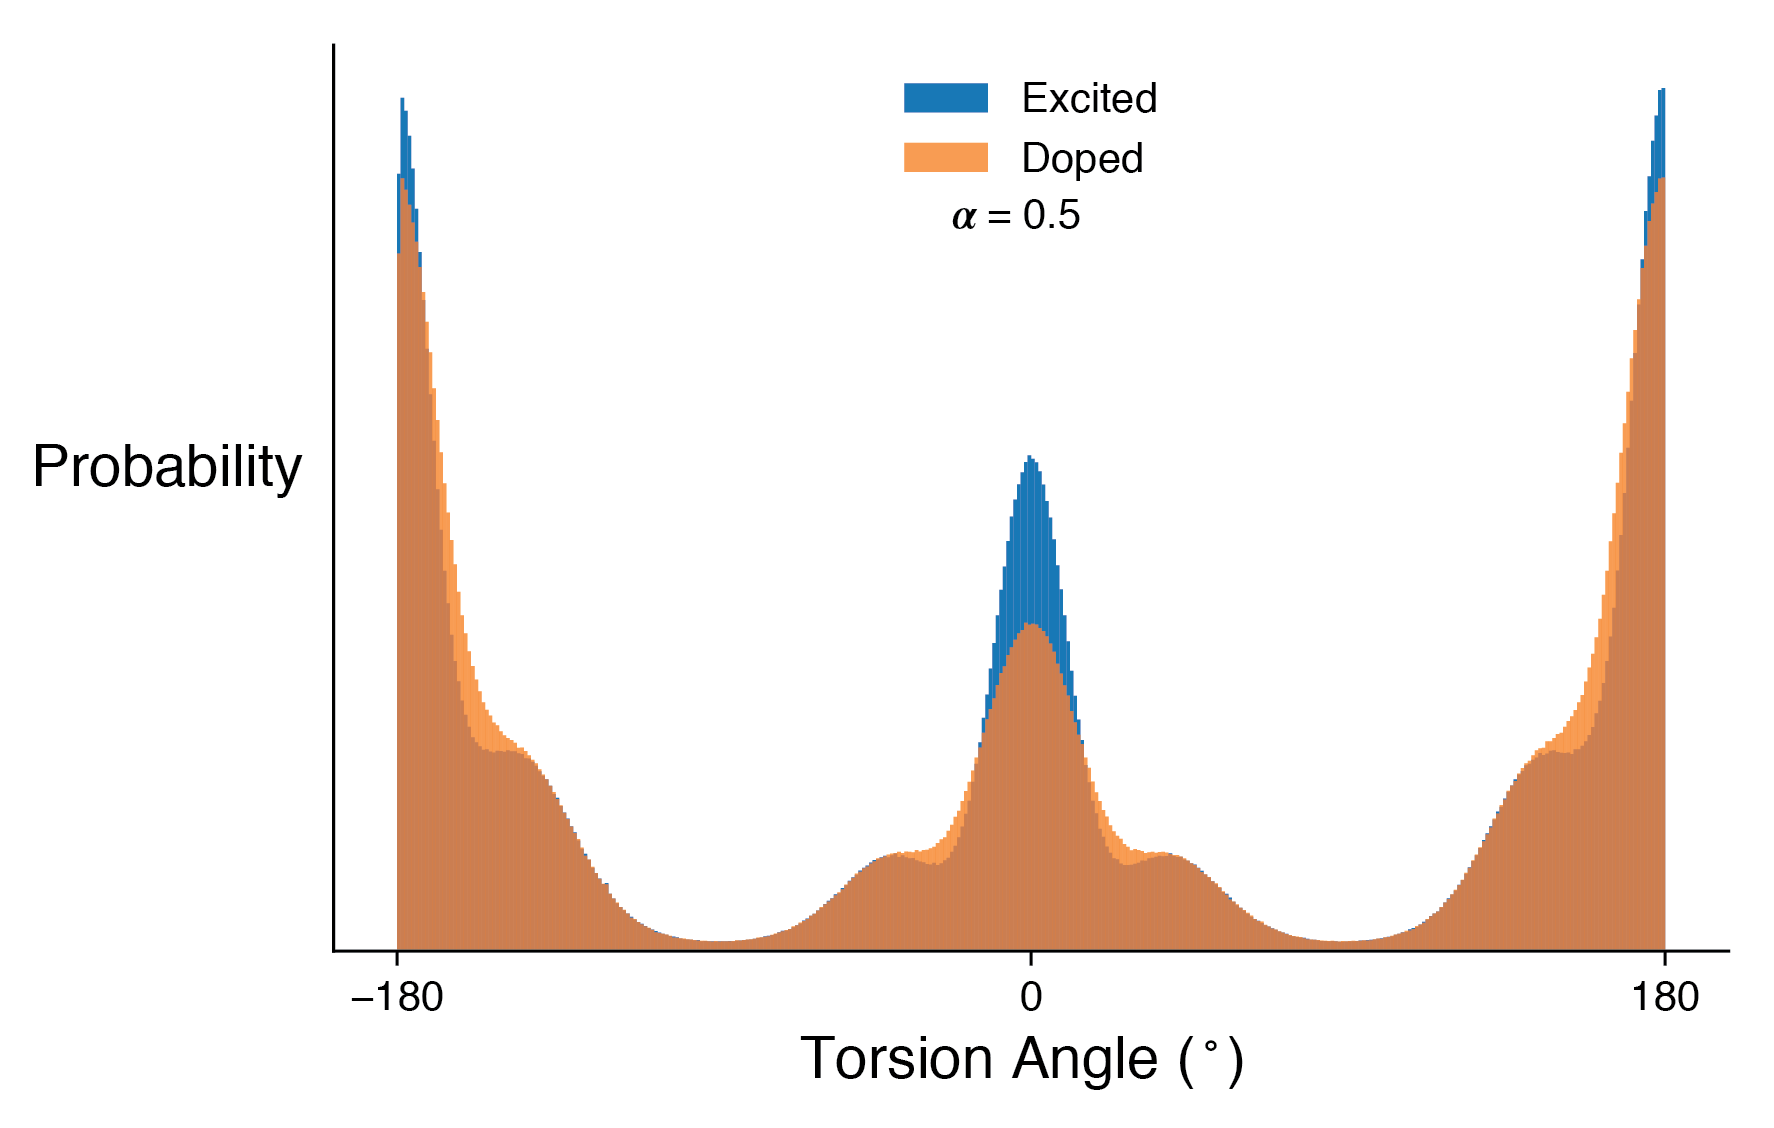
\includegraphics{figures/append_tor_model/a_050_hist.png}
    \caption[Histogram of Doped and Excited Sampled Torsion Angles at $\alpha = 0.5$]{Overlaid histograms of doped and excited sampled torsion angles at $\alpha = 0.5$}
    \label{fig:a_050_hist}
\end{figure}

\begin{figure}[hbt!]
    \centering
    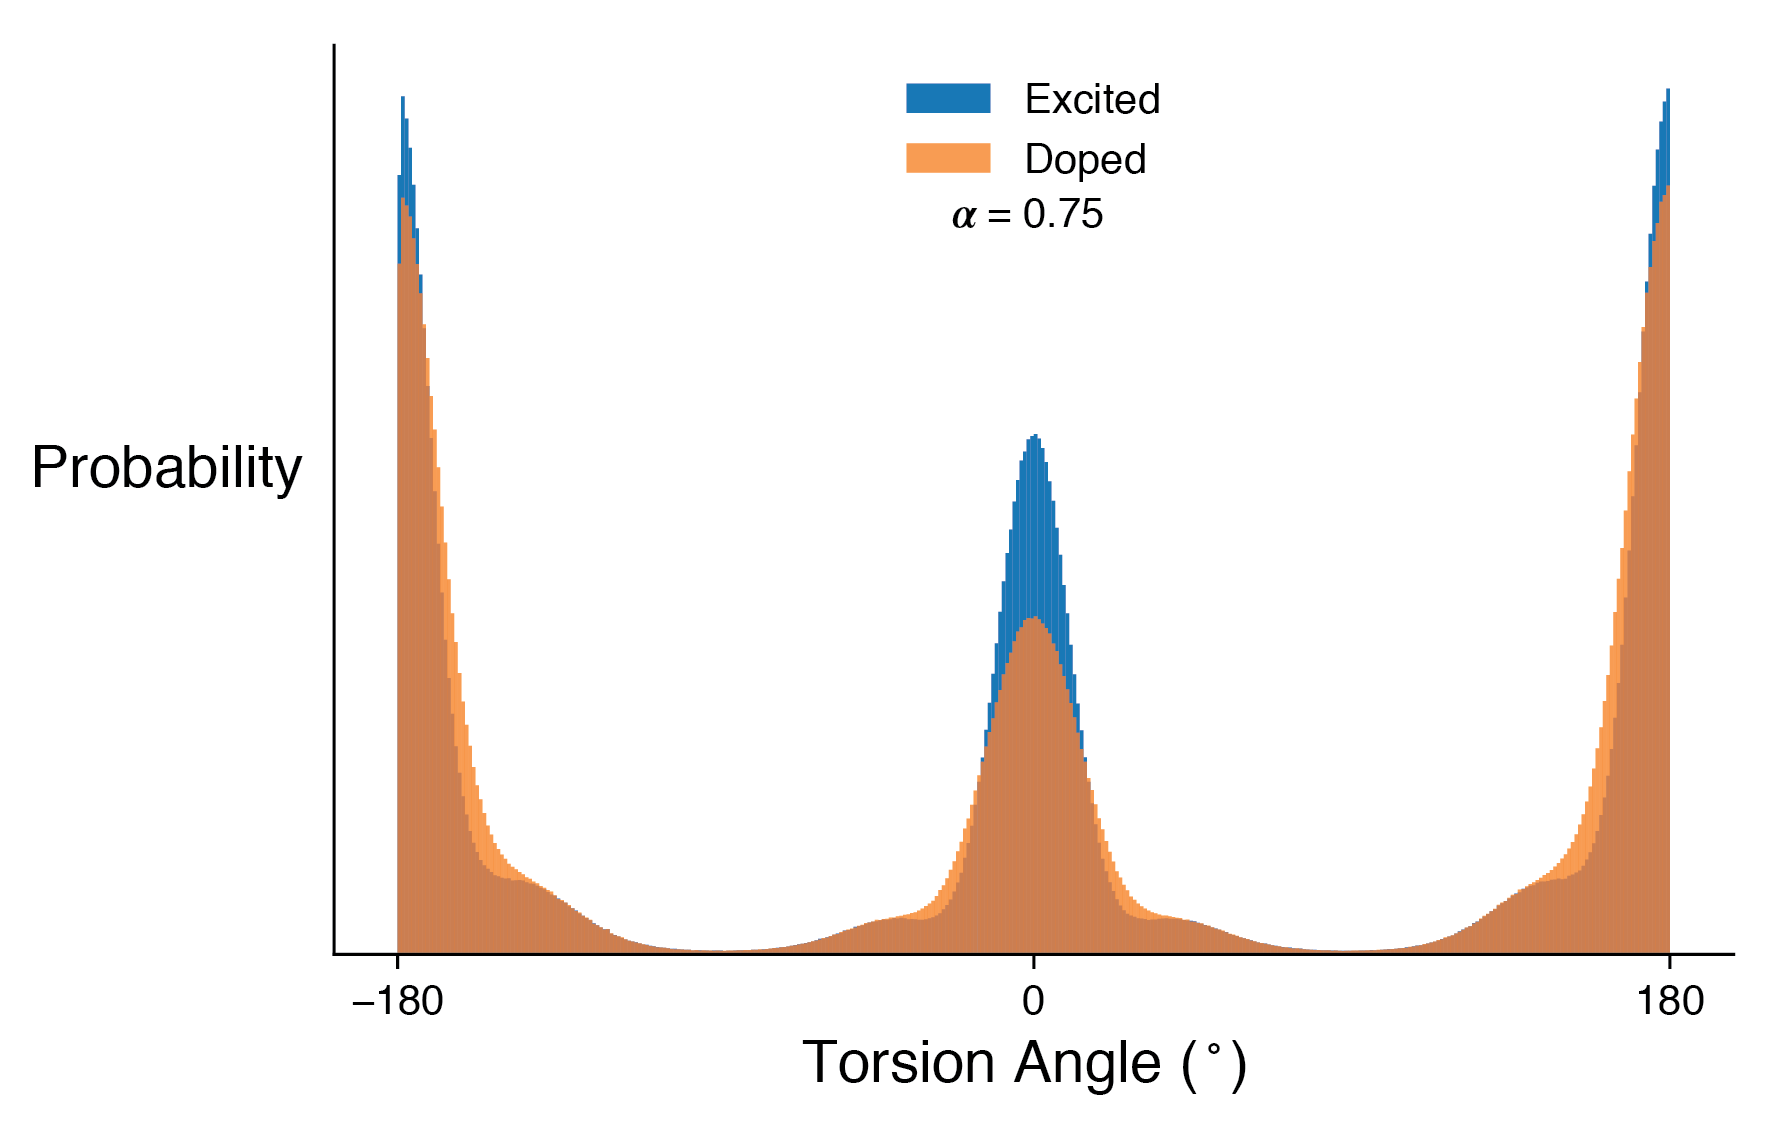
\includegraphics{figures/append_tor_model/a_075_hist.png}
    \caption[Histogram of Doped and Excited Sampled Torsion Angles at $\alpha = 0.75$]{Overlaid histograms of doped and excited sampled torsion angles at $\alpha = 0.75$}
    \label{fig:a_075_hist}
\end{figure}

\begin{figure}[hbt!]
    \centering
    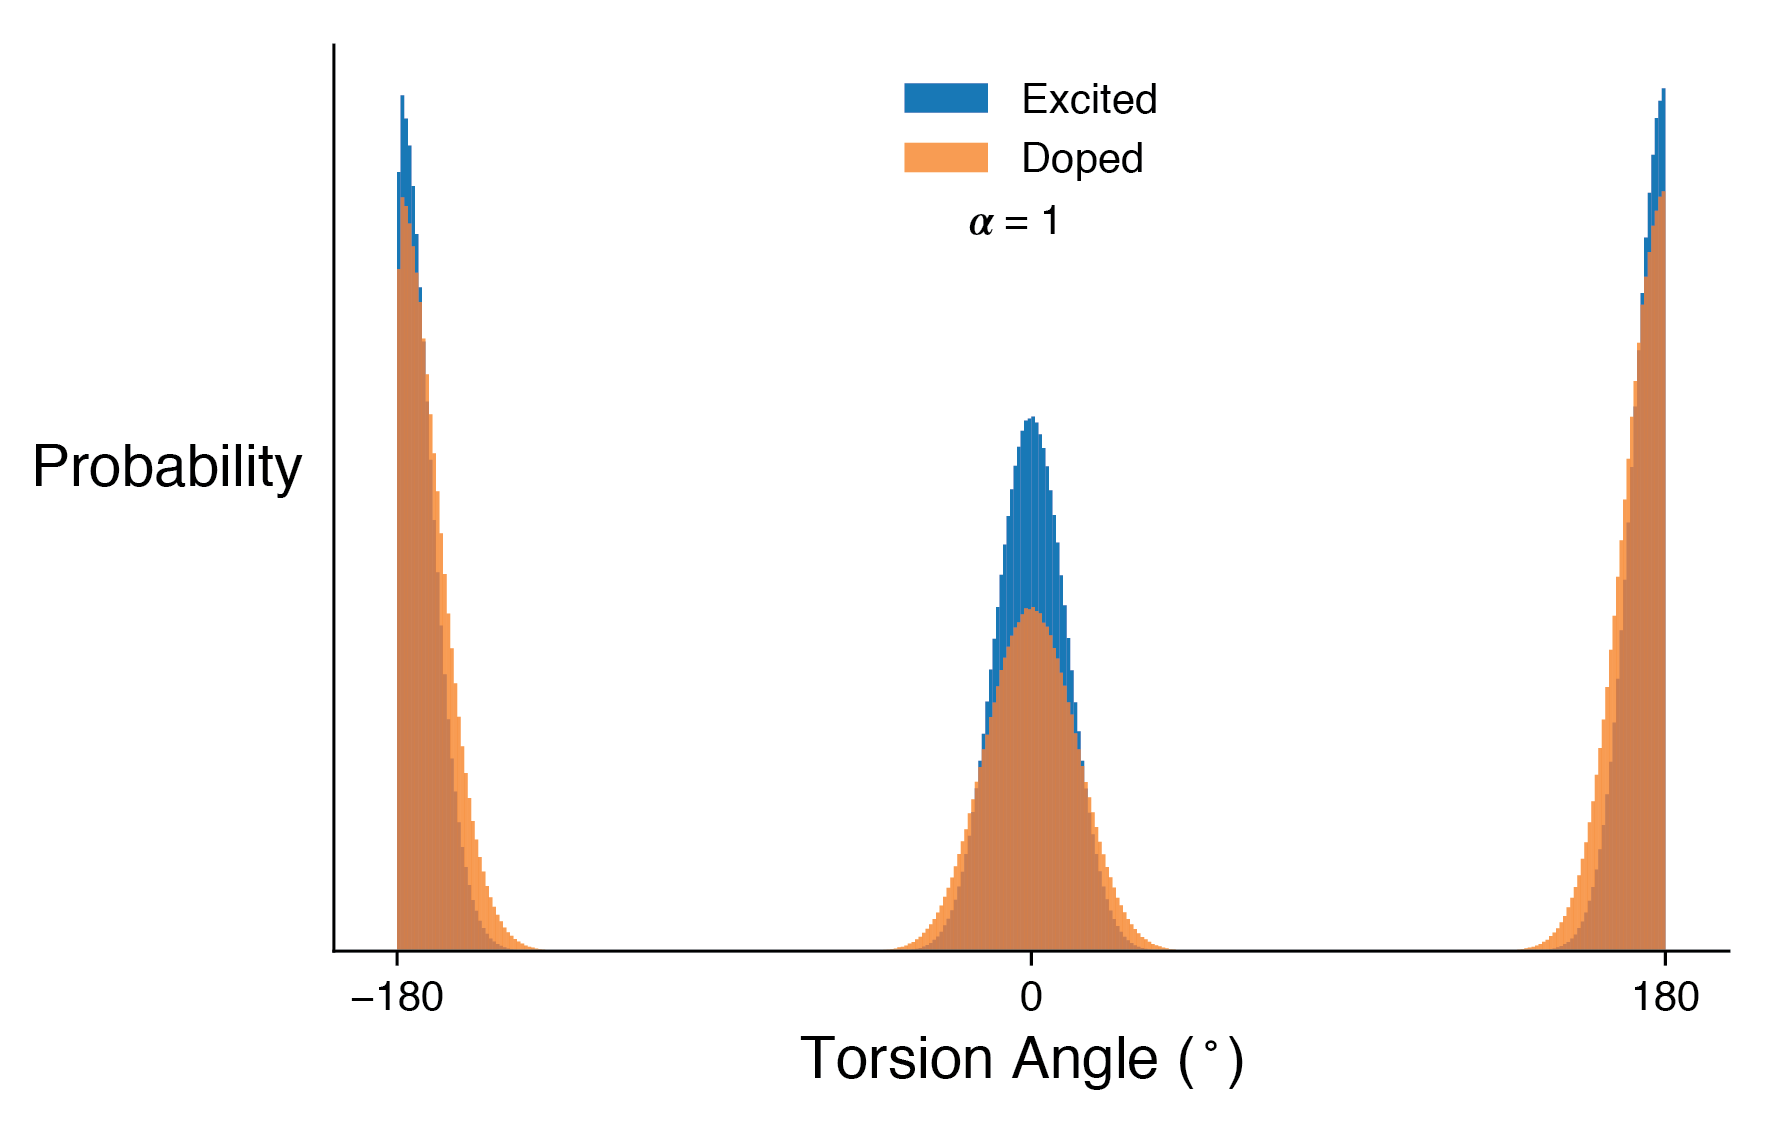
\includegraphics{figures/append_tor_model/a_1_hist.png}
    \caption[Histogram of Doped and Excited Sampled Torsion Angles at $\alpha = 1$]{Overlaid histograms of doped and excited sampled torsion angles at $\alpha = 1$}
    \label{fig:a_1_hist}
\end{figure}

\clearpage
\section{Planarity}
\label{sec:planarity}
\subsection{Orientational Order Tensor}

The second rank orientational order tensor Q (Eq.~\ref{eq:Q}) was used to calculate the director and the S order parameter for each chain. The vectors used to describe chain planarity were the unit normal vectors ($\hat{e}$) to each thiophene ring along the chain (depicted in Fig.~\ref{fig:pt_vecs}). In Eq.~\ref{eq:Q}, $\hat{e} \otimes \hat{e}$ represents the outer product, which is equivalent to matrix multiplication of the column vector $\hat{e}$ and row vector $\hat{e}$. Additionally, $\mathds{1}$ represents the identity matrix. The parameter S and the director were determined by diagonalizing Q, where S is the largest eigenvalue and the director is the corresponding eigenvector \cite{Allen2017}.

\begin{equation}
\Large
\overleftrightarrow{Q} = \frac{1}{2N} \sum_{i=1}^{N} 3\hat{e_i} \otimes \hat{e_i} - \mathds{1}
\label{eq:Q}
\end{equation}

\chapter{Appendix for Aromaticity as a Guide to Planarity in Conjugated Molecules and Polymers}

\section{Different Length Polymer Chains}\label{sec:aroma_diff_len_poly}
\begin{figure}[hbt!]
    \centering
    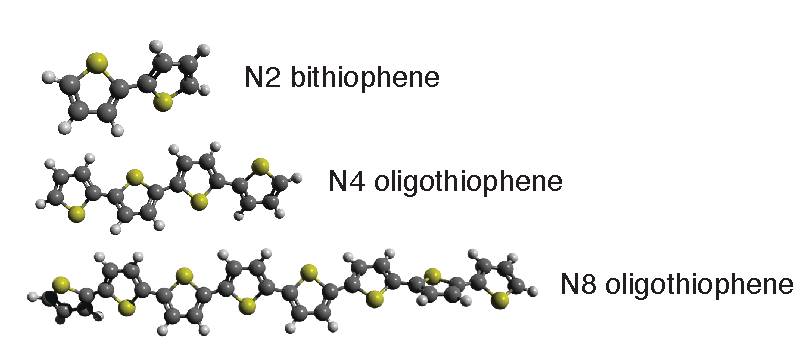
\includegraphics{figures/append_aroma/p_chains_graphic_copy.pdf}
    \caption{Different length oligomers of thiophene.}
    \label{fig:p_chains}
\end{figure}

\subsection{Comparison of Torsion Potentials}
\begin{figure}[hbt!]
    \centering
    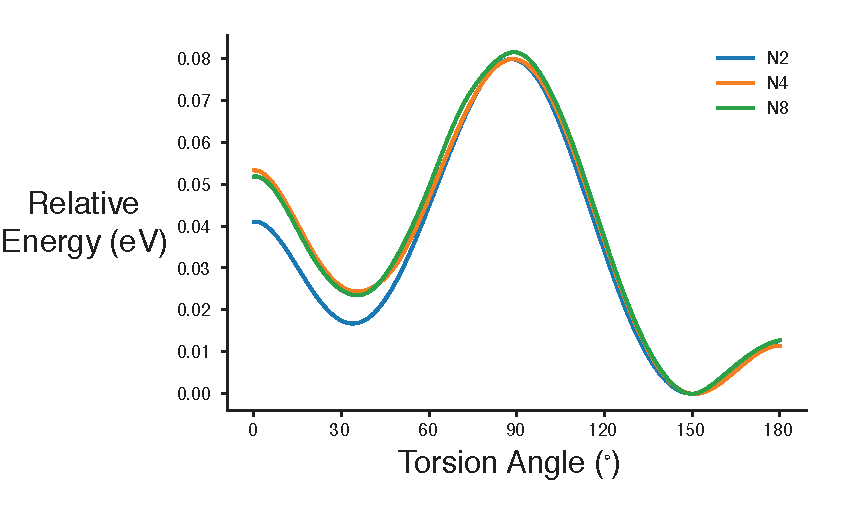
\includegraphics{figures/append_aroma/p_tor_compare_copy.pdf}
    \caption{The torsion potential of N2, N4, and N8 thiophene oligomers. All calculations were performed using the $\omega$B97x-D functional. The N2 torsion potential was calculated with the def2-TZVPP basis set, while N4 and N8 utilized the 6-31++G**\cite{Hehre1972} basis set to reduce to the computational cost. The deviation of N2 from both N4 and N8 between 0 and 50\textdegree \ is likely due to the different basis sets employed.}
    \label{fig:p_tor_compare}
\end{figure}

\clearpage
\subsection{Comparison of NICS Aromaticity}
\begin{figure}[hbt!]
    \centering
    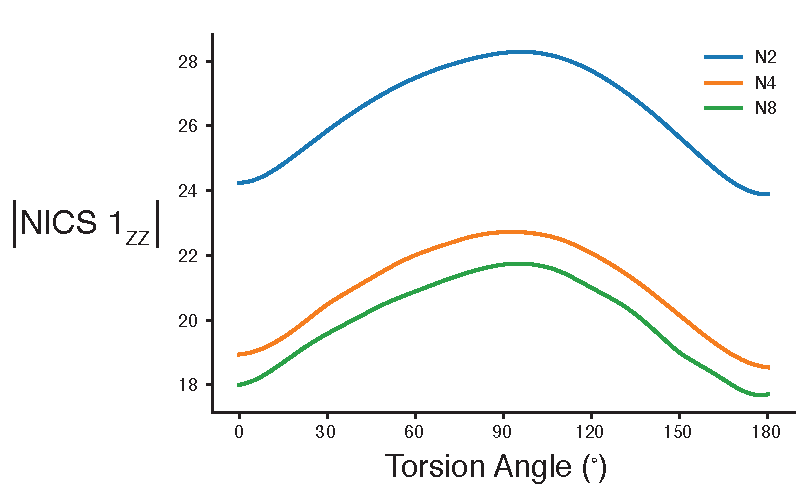
\includegraphics{figures/append_aroma/p_NICS_compare_copy.pdf}
    \caption{N2, N4, and N8 absolute NICS $1_{ZZ}$ values as a function of torsion angle. The magnitude of NICS values decrease with chain length, and we expect that the values will converge once a certain chain length is reached. While the magnitude decreases the overall trend as a function of torsion angle is consistent, which allows N2 to represent larger chains.}
    \label{fig:p_NICS_compare}
\end{figure}

\clearpage
\section{Comparision of MCI and NICS Aromaticity Values}\label{sec:aroma_mci_nics_comp}

\subsection{BT}
\begin{figure}[hbt!]
    \centering
    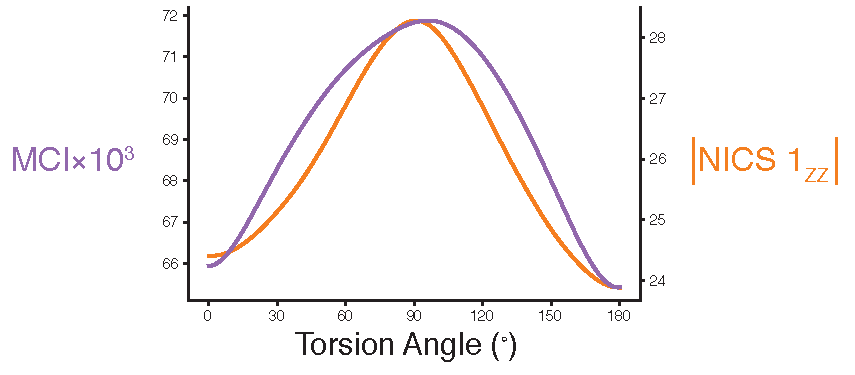
\includegraphics{figures/append_aroma/pt_aroma_compare_copy.pdf}
    \caption{Comparison of the aromaticity indexes MCI and NICS for BT.}
    \label{fig:pt_aroma_compare}
\end{figure}

\subsection{hBT}
\begin{figure}[hbt!]
    \centering
    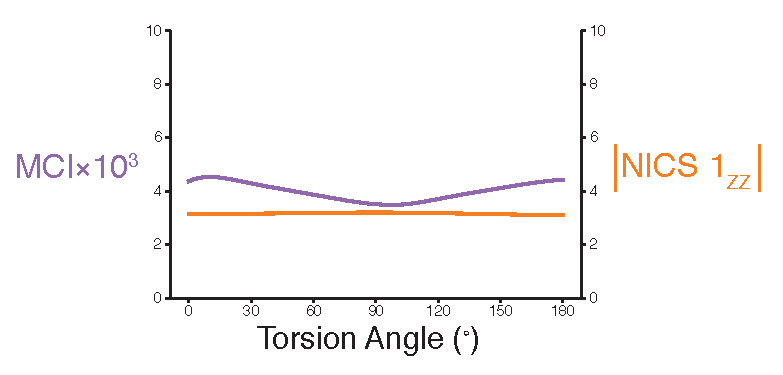
\includegraphics{figures/append_aroma/hpt_aroma_compare_copy.pdf}
    \caption{Comparison of the aromaticity indexes MCI and NICS for hBT.}
    \label{fig:hpt_aroma_compare}
\end{figure}

\clearpage
\subsection{F2-BT}
\begin{figure}[hbt!]
    \centering
    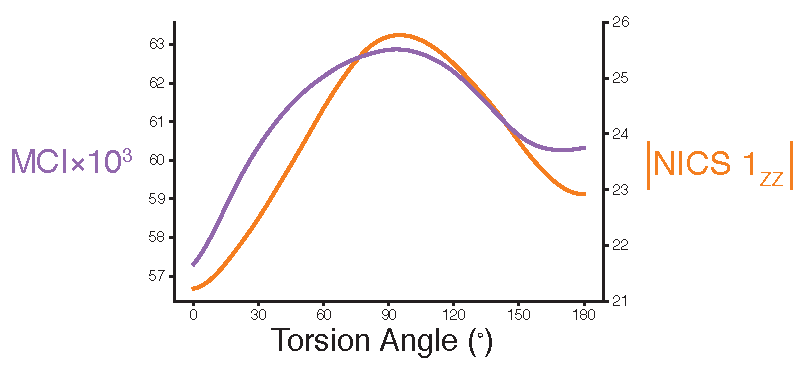
\includegraphics{figures/append_aroma/pt_f2_aroma_compare_copy.pdf}
    \caption{Comparison of the aromaticity indexes MCI and NICS for F2-BT.}
    \label{fig:pt_f2_aroma_compare}
\end{figure}


\subsection{BEDOT}
\begin{figure}[hbt!]
    \centering
    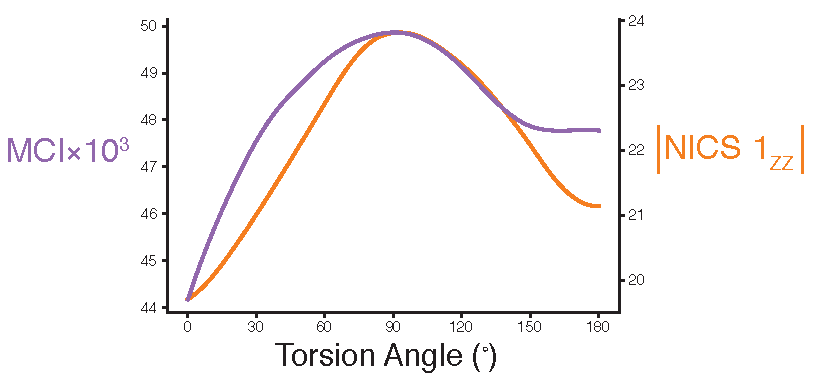
\includegraphics{figures/append_aroma/pedot_aroma_compare_copy.pdf}
    \caption{Comparison of the aromaticity indexes MCI and NICS for BEDOT.}
    \label{fig:pedot_aroma_compare}
\end{figure}

\clearpage
\section{Through-space Calculations}\label{sec:aroma_ts}
\subsection{\texorpdfstring{H $\cdots$ S}{HS}}
\begin{figure}[hbt!]
    \centering
    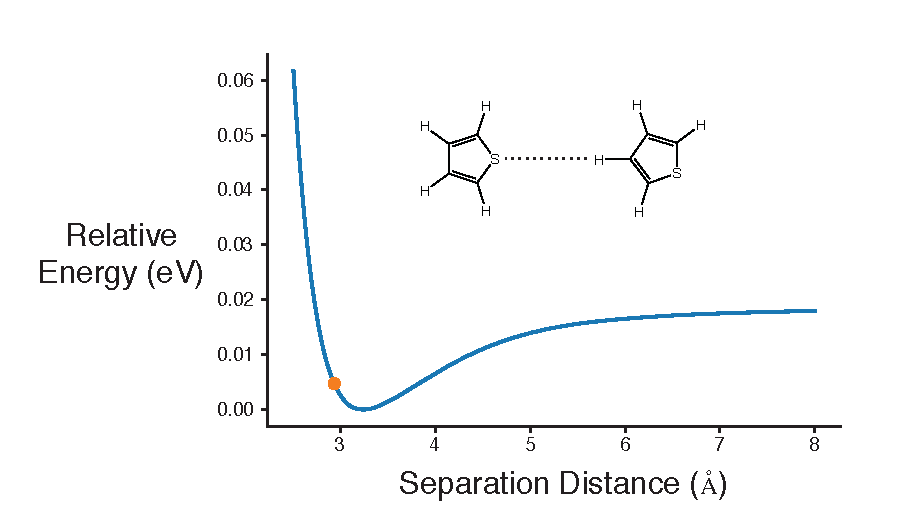
\includegraphics{figures/append_aroma/ts_t_t_copy.pdf}
    \caption{A potential energy scan of the interatomic separation distance between a hydrogen and a sulfur atom on thiophene molecules. The orange dot represents the relaxed H $\cdots$ S distance on a trans (180\textdegree) BT molecule. This indicates that the H $\cdots$ S through-space interaction is marginally repulsive in trans BT. It is noteworthy that the repulsive energy is small compared to the torsional barrier present at 180\textdegree \ in BT (a factor of $\sim$2.5), which in combination with the NCI analysis below demonstrate the minor role of sterics in determining planarity.}
    \label{fig:ts_t_t}
\end{figure}
\clearpage

\subsection{\texorpdfstring{H $\cdots$ S}{HSN} Noncovalent Interaction Analysis}
\begin{figure}[hbt!]
    \centering
    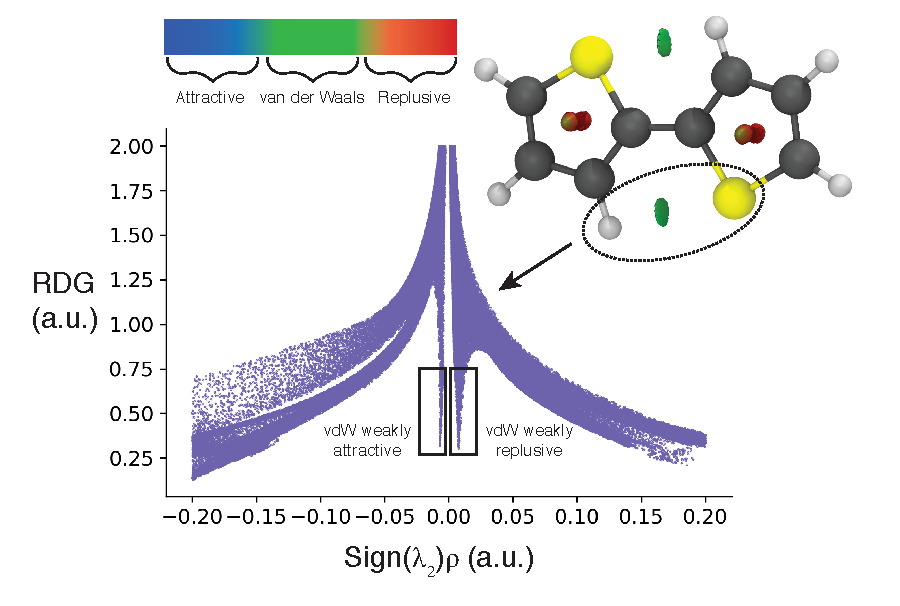
\includegraphics{figures/append_aroma/pt_nci_copy.pdf}
    \caption{The NCI analysis of BT including an NCI isosurface (right) and an s$(\rho$) plot (center), which displays the reduced density gradient (RDG) as a function of the sign of the electron-density Hessian matrix's second eiganvalue (sign$(\lambda_{2})$) times the electron-density ($\rho$). The isosurface plot on right shows a van der Waals interaction between H $\cdots$ S. The color gradient at the top gives a rough physical description of the color scheme used for the isosurface. When only the localized region around H $\cdots$ S is considered, by employing a radius cutoff, the s$(\rho$) plot is inconclusive exhibiting both weakly repulsive and weakly attractive interactions.}
    \label{fig:pt_nci}
\end{figure}
\clearpage

\subsection{\texorpdfstring{F $\cdots$ S}{FS}}
\begin{figure}[hbt!]
    \centering
    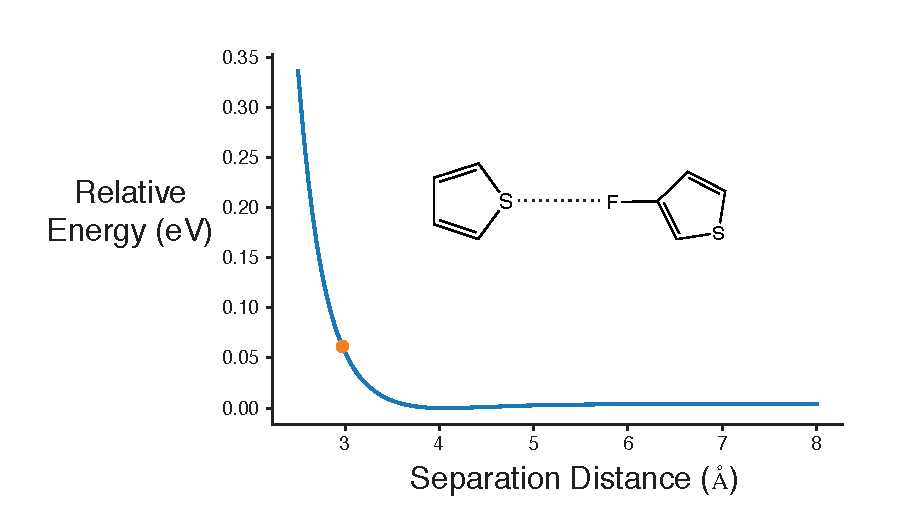
\includegraphics{figures/append_aroma/ts_t_t_f1_copy.pdf}
    \caption{A potential energy scan of the interatomic separation distance between a fluoride and a sulfur atom on a fluorinated thiophene and a thiophene molecule. The orange dot represents the relaxed F $\cdots$ S distance on a trans (180\textdegree) 3F-BT molecule. This indicates that the F $\cdots$ S through-space interaction is repulsive in trans 3F-BT.}
    \label{fig:ts_t_t_f1}
\end{figure}

\begin{figure}[hbt!]
    \centering
    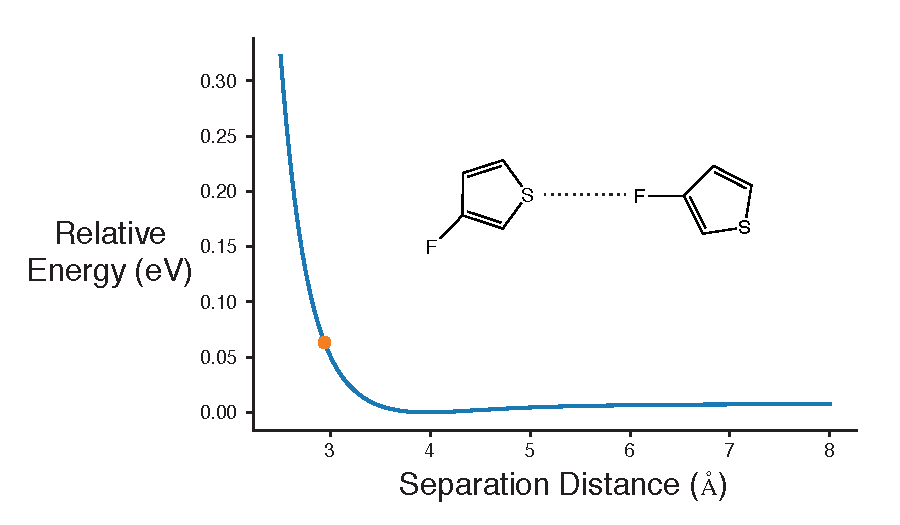
\includegraphics{figures/append_aroma/ts_2t_f1_copy.pdf}
    \caption{A potential energy scan of the interatomic separation distance between a fluoride and a sulfur atom on a fluorinated thiophene molecules. The orange dot represents the relaxed F $\cdots$ S distance on a trans (180\textdegree) F2-BT molecule. This indicates that the F $\cdots$ S through-space interaction is repulsive in trans F2-BT.}
    \label{fig:ts_2t_f1}
\end{figure}
\clearpage

\subsection{\texorpdfstring{F $\cdots$ S}{FSN} Noncovalent Interaction Analysis}
\begin{figure}[hbt!]
    \centering
    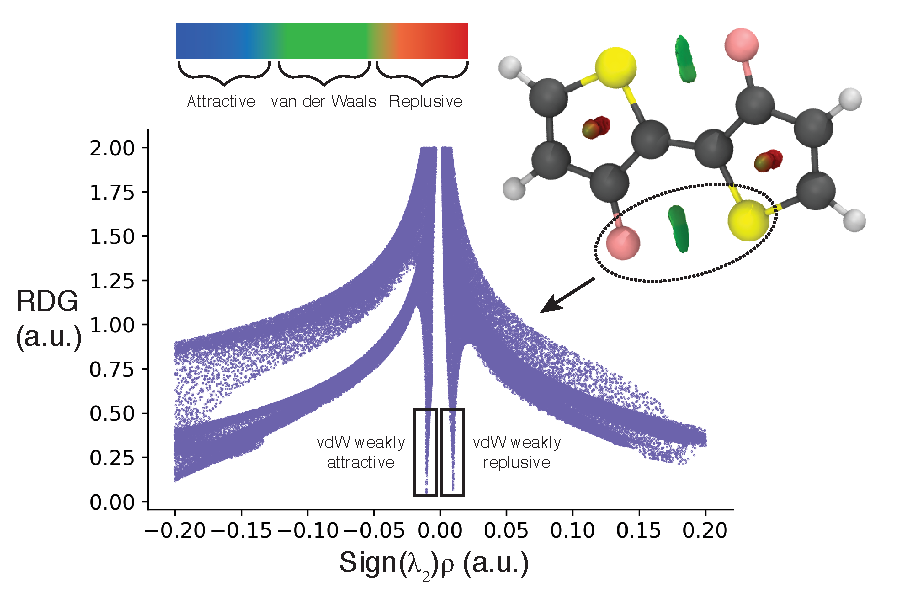
\includegraphics{figures/append_aroma/pt_f2_nciplot_copy.pdf}
    \caption{The NCI analysis of F2-BT including an NCI isosurface (right) and an s$(\rho$) plot (center), which displays the reduced density gradient (RDG) as a function of the sign of the electron-density Hessian matrix's second eiganvalue (sign$(\lambda_{2})$) times the electron-density ($\rho$). The isosurface plot on right shows a van der Waals interaction between H $\cdots$ S. The color gradient at the top gives a rough physical description of the color scheme used for the isosurface. When only the localized region around H $\cdots$ S is considered, by employing a radius cutoff, the s$(\rho$) plot is inconclusive exhibiting both weakly repulsive and weakly attractive interactions.}
    \label{fig:pt_f2_nci}
\end{figure}
\clearpage

\subsection{\texorpdfstring{O $\cdots$ S}{OS}}
\begin{figure}[hbt!]
    \centering
    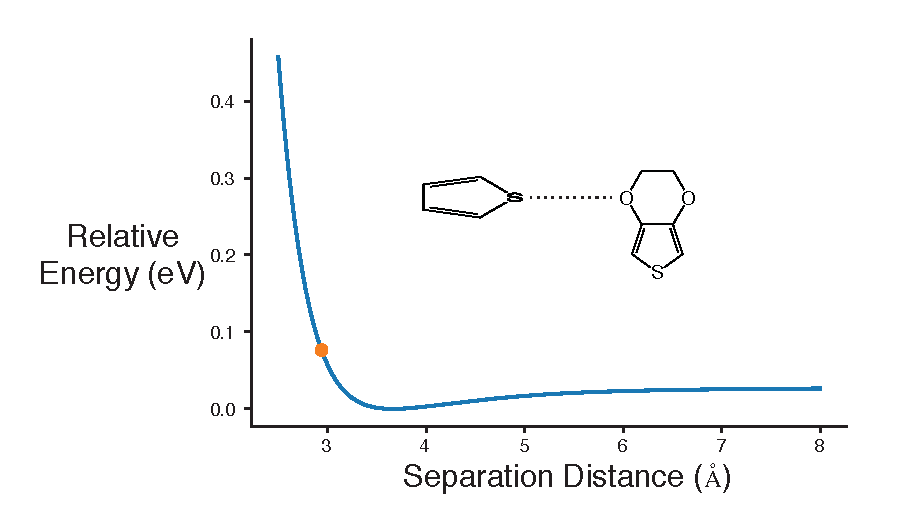
\includegraphics{figures/append_aroma/ts_t_edot_copy.pdf}
    \caption{A potential energy scan of the interatomic separation distance between a oxygen and a sulfur atom on an EDOT and thiophene molecule respectively. The thiophene molecule has been rotated such that the ring is perpendicular to the EDOT, this is done to minimize secondary H $\cdots$ S interactions. The orange dot represents the relaxed O $\cdots$ S distance on a trans (180\textdegree) BEDOT molecule. This indicates that the O $\cdots$ S through-space interaction is repulsive in trans BEDOT.}
    \label{fig:ts_t_edot}
\end{figure}
\clearpage

\subsection{\texorpdfstring{O $\cdots$ S}{OSN} Noncovalent Interaction Analysis}
\begin{figure}[hbt!]
    \centering
    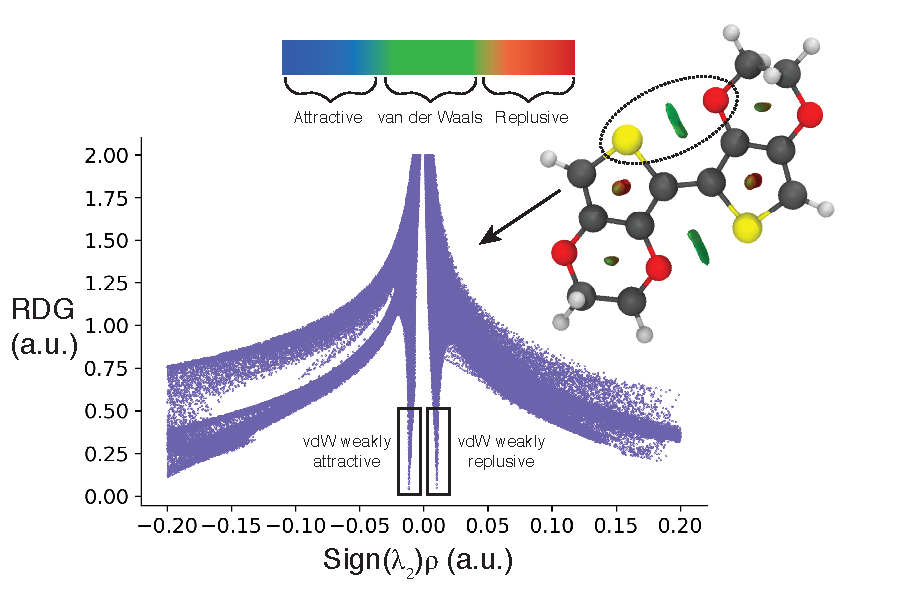
\includegraphics{figures/append_aroma/pedot_nciplot_copy.pdf}
    \caption{The NCI analysis of BEDOT including an NCI isosurface (right) and an s$(\rho$) plot (center), which displays the reduced density gradient (RDG) as a function of the sign of the electron-density Hessian matrix's second eiganvalue (sign$(\lambda_{2})$) times the electron-density ($\rho$). The isosurface plot on right shows a van der Waals interaction between H $\cdots$ S. The color gradient at the top gives a rough physical description of the color scheme used for the isosurface. When only the localized region around H $\cdots$ S is considered, by employing a radius cutoff, the s$(\rho$) plot is inconclusive exhibiting both weakly repulsive and weakly attractive interactions.}
    \label{fig:pedot_nci}
\end{figure}
\clearpage

%%%%%%%%%%%%%%%%%%%%%%%%%%
\section{NBO Perturbation Analysis}\label{sec:aroma_nbo_e2}

\begin{table}[hbt!]\centering
\caption{NBO Stabilization Energies}
\label{tab:tpm_vals}
\renewcommand{\arraystretch}{1.5}
\begin{threeparttable}
\begin{tabular}{cccc}\toprule
\multicolumn{1}{c}{\multirow{2}{2.5cm}{\centering }} &
\multicolumn{1}{c}{\multirow{2}{1.5cm}{\centering Donor}} &
\multicolumn{1}{c}{\multirow{2}{1.6cm}{\centering Acceptor}} &
\multicolumn{1}{c}{\multirow{2}{5.5cm}{\centering Stabilization Energy E(2) \\ kcal/mol}} \\ \\ \midrule
    F2-BT\tnote{$\dagger$} & $LP_F$ & $\sigma^{*}_{C-S}$ & 0.84\\
    BEDOT\tnote{$\dagger$} & $LP_O$ & $\sigma^{*}_{C-S}$ & 1.09\\ \bottomrule
\end{tabular}
\begin{tablenotes}
\item[$\dagger$] \footnotesize Energy values represent 180\textdegree \ configurations
\end{tablenotes}
\end{threeparttable}
\end{table}

%%%%%%%%%%%%%%%%%%%%%%%%%%
\section{Expanded Methods}\label{sec:aroma_exp_method}

\subsection{Hydrogenation of BT}
Additional torsional constraints were placed on the hBT dimer during geometry optimizations to prevent ring distortion. The intent of hydrogenation was to remove aromaticity, while maintaining conjugation across the central C-C bond between rings. Ring distortion is an unintended consequence of hydrogenation and does not represent the physics of interest. As a result, the intra-ring C-C-C-C torsion angle for each thiophene ring was fixed at its undistorted state (roughly 0\textdegree), in addition to the central inter-ring C-C-C-C torsion angle being fixed at the desired angle within the potential energy scan. In sum, geometry optimizations for the hBT dimer had 3 torsional constraints, 2 intra-ring and 1 inter-ring, whereas all other degrees of freedom were allowed to relax.

\subsection{NICS Calculations}
NICS values were computed by placing fictitious hydrogen atoms (designated H-Bq in Gaussian) 1\si{\angstrom} above the center of each ring, followed by an NMR calculation with Gaussian16.\cite{g16} The largest eigenvalue of the magnetic shielding tensor for the fictitious H atom was taken as the NICS $1_{ZZ}$ value in ppm. Conventionally, the sign of NICS values are reversed for comparison with experimental NMR values. In this work we do not reverse the sign and report the absolute NICS $1_{ZZ}$ value ($\abs*{NICS 1_{ZZ}}$) for easy comparison with MCI aromaticity values. Specific details on the NICS method have been described elsewhere.\cite{Fallah-Bagher-Shaidaei2006, Chen2005}

\subsection{Through-space Calculations}
All through-space potential energy scans utilized counterpoise corrected energies as implementation in Gaussian16. Methodology of through-space calculations has been described by others.\cite{Jackson2013}

\subsection{NCI Analysis}
NCI analysis was preformed with NCIplot.\cite{Johnson2010, Contreras-Garcia2011} The only deviation from standard procedure was adding a radius cutoff to investigate local interactions (i.e. X $\cdots$ S). For these calculations a point was specified roughly half way between the two atoms with a radius cutoff of 2\AA.

\clearpage
%%%%%%%%%%%%%%%%%%%%%%%%%%
\section{Tabular Data}

\subsection{BT}
%\subsubsection{Energy, Aromaticity, and Conjugation Data}
\begin{table}[hbt!]\centering
\caption{Bithiophene Torsional Data}
\renewcommand{\arraystretch}{1.5}
\begin{threeparttable}
\begin{tabular}{cccccc}\toprule
\multicolumn{1}{c}{\multirow{2}{2.0cm}{\centering Torsion \\ Angle (\textdegree)}} &
\multicolumn{1}{c}{\multirow{2}{2.2cm}{\centering Rel. Energy (eV)}} &
\multicolumn{1}{c}{\multirow{2}{2.5cm}{\centering Abs. Energy \\ (Hartree)}} &
\multicolumn{1}{c}{\multirow{2}{1.5cm}{\centering MCI $\times 10^3$}\tnote{$\dagger$}} &
\multicolumn{1}{c}{\multirow{2}{1.5cm}{\centering $\abs*{\bfrac{NICS} {1_{ZZ}}}$}\tnote{$\ddagger$}} &
\multicolumn{1}{c}{\multirow{2}{2.5cm}{\centering Central Bond \\ Length (\AA)}}
\\ \\ \midrule
    0.0 & 0.04106 & -1104.84898 & 66.19 (66.18) & 24.24 (24.24) & 1.455 \\
    10.0 & 0.03557 & -1104.84919 & 66.30 (66.32) & 24.53 (24.50) & 1.455 \\
    20.0 & 0.02465 & -1104.84959 & 66.69 (66.67) & 25.15 (25.14) & 1.454 \\
    30.0 & 0.01742 & -1104.84985 & 67.25 (67.25) & 25.85 (25.84) & 1.455 \\
    40.0 & 0.01849 & -1104.84981 & 67.96 (67.98) & 26.48 (26.48) & 1.456 \\
    50.0 & 0.02854 & -1104.84944 & 68.83 (68.82) & 27.03 (27.04) & 1.458 \\
    60.0 & 0.04480 & -1104.84885 & 69.83 (69.82) & 27.48 (27.48) & 1.460 \\
    70.0 & 0.06250 & -1104.84820 & 70.80 (70.77) & 27.83 (27.82) & 1.463 \\
    80.0 & 0.07593 & -1104.84770 & 71.54 (71.53) & 28.09 (28.08) & 1.465 \\
    90.0 & 0.07962 & -1104.84757 & 71.88 (71.87) & 28.25 (28.26) & 1.466 \\
    100.0 & 0.07169 & -1104.84786 & 71.60 (71.60) & 28.27 (28.28) & 1.465 \\
    110.0 & 0.05443 & -1104.84849 & 70.81 (70.83) & 28.08 (28.09) & 1.463 \\
    120.0 & 0.03391 & -1104.84925 & 69.80 (69.79) & 27.70 (27.72) & 1.460 \\
    130.0 & 0.01566 & -1104.84992 & 68.71 (68.72) & 27.14 (27.16) & 1.458 \\
    140.0 & 0.00386 & -1104.85035 & 67.71 (67.71) & 26.44 (26.45) & 1.456 \\
    150.0 & 0.00000 & -1104.85049 & 66.82 (66.82) & 25.64 (25.66) & 1.454 \\
    160.0 & 0.00284 & -1104.85039 & 66.12 (66.11) & 24.82 (24.83) & 1.454 \\
    170.0 & 0.00864 & -1104.85018 & 65.61 (65.60) & 24.15 (24.15) & 1.454 \\
    180.0 & 0.01147 & -1104.85007 & 65.42 (65.43) & 23.88 (23.88) & 1.454 \\ \bottomrule
\end{tabular}
\begin{tablenotes}
\item[*] \footnotesize All quantum calculations employed the $\omega$B97x-D functional with the def2-TZVPP basis set.
\item [$\dagger$] \footnotesize The MCI values in parentheses represent the second ring in the dimer molecule.
\item [$\ddagger$] \footnotesize The units of NICS values are ppm, and for comparison with MCI we have not reversed the sign. The NICS values in parentheses represent the second ring in the dimer molecule.
\end{tablenotes}
\end{threeparttable}
\end{table}

%\subsubsection{Relaxed Structure}
\begin{table}[hbt!]\centering
\caption{Bithiophene Relaxed Structure}
\renewcommand{\arraystretch}{1.5}
\begin{threeparttable}
\begin{tabular}{ccccc}\toprule
{} & {Atom} & {x (\AA)} & {y (\AA)} & {z (\AA)} \\ \midrule
    1 & S & 0.001 & -0.024 & -0.030\\
    2 & C & 1.708 & -0.014 & -0.014\\
    3 & H & 2.244 & -0.025 & 0.920\\
    4 & C & 2.219 & 0.008 & -1.274\\
    5 & H & 3.277 & 0.017 & -1.488\\
    6 & C & 1.210 & 0.029 & -2.269\\
    7 & H & 1.409 & 0.069 & -3.330\\
    8 & C & -0.054 & 0.021 & -1.750\\
    9 & C & -1.326 & 0.042 & -2.457\\
    10 & C & -2.520 & 0.567 & -2.048\\
    11 & H & -2.646 & 1.070 & -1.100\\
    12 & C & -3.553 & 0.408 & -3.004\\
    13 & H & -4.563 & 0.763 & -2.865\\
    14 & C & -3.130 & -0.234 & -4.126\\
    15 & H & -3.701 & -0.478 & -5.006\\
    16 & S & -1.481 & -0.662 & -4.020\\ \bottomrule
\end{tabular}
\begin{tablenotes}
\item[*] \footnotesize Level of theory: $\omega$B97x-D \\ Basis set: def2-TZVPP
\end{tablenotes}
\end{threeparttable}
\end{table}

\clearpage
\subsection{hBT}

\begin{table}[hbt!]\centering
\caption{Hydrogenated Bithiophene Torsional Data}
\renewcommand{\arraystretch}{1.5}
\begin{threeparttable}
\begin{tabular}{cccccc}\toprule
\multicolumn{1}{c}{\multirow{2}{2.0cm}{\centering Torsion \\ Angle (\textdegree)}} &
\multicolumn{1}{c}{\multirow{2}{2.2cm}{\centering Rel. Energy (eV)}} &
\multicolumn{1}{c}{\multirow{2}{2.5cm}{\centering Abs. Energy \\ (Hartree)}} &
\multicolumn{1}{c}{\multirow{2}{1.5cm}{\centering MCI $\times 10^3$}\tnote{$\dagger$}} &
\multicolumn{1}{c}{\multirow{2}{1.5cm}{\centering $\abs*{\bfrac{NICS} {1_{ZZ}}}$}\tnote{$\ddagger$}} &
\multicolumn{1}{c}{\multirow{2}{2.5cm}{\centering Central Bond \\ Length (\AA)}}
\\ \\ \midrule
0.0 & 0.16920 & -1107.25114 & 3.16 (3.16) & 4.38 (4.37) & 1.468 \\
10.0 & 0.15361 & -1107.25172 & 3.15 (3.15) & 4.53 (4.54) & 1.467 \\
20.0 & 0.12613 & -1107.25273 & 3.15 (3.15) & 4.45 (4.45) & 1.465 \\
30.0 & 0.10310 & -1107.25357 & 3.16 (3.16) & 4.30 (4.29) & 1.463 \\
40.0 & 0.09123 & -1107.25401 & 3.17 (3.17) & 4.15 (4.15) & 1.462 \\
50.0 & 0.09212 & -1107.25398 & 3.18 (3.18) & 4.01 (4.01) & 1.463 \\
60.0 & 0.10437 & -1107.25353 & 3.19 (3.19) & 3.88 (3.87) & 1.464 \\
70.0 & 0.12360 & -1107.25282 & 3.20 (3.20) & 3.74 (3.73) & 1.466 \\
80.0 & 0.14340 & -1107.25209 & 3.20 (3.20) & 3.62 (3.60) & 1.469 \\
90.0 & 0.15647 & -1107.25161 & 3.21 (3.21) & 3.53 (3.51) & 1.471 \\
100.0 & 0.15718 & -1107.25158 & 3.20 (3.20) & 3.51 (3.49) & 1.472 \\
110.0 & 0.14297 & -1107.25211 & 3.19 (3.19) & 3.59 (3.57) & 1.471 \\
120.0 & 0.11631 & -1107.25309 & 3.18 (3.18) & 3.72 (3.71) & 1.469 \\
130.0 & 0.08418 & -1107.25427 & 3.16 (3.16) & 3.86 (3.86) & 1.465 \\
140.0 & 0.05374 & -1107.25539 & 3.15 (3.15) & 4.00 (3.99) & 1.462 \\
150.0 & 0.02927 & -1107.25629 & 3.13 (3.13) & 4.13 (4.12) & 1.459 \\
160.0 & 0.01226 & -1107.25691 & 3.12 (3.12) & 4.25 (4.25) & 1.457 \\
170.0 & 0.00288 & -1107.25725 & 3.11 (3.11) & 4.37 (4.36) & 1.456 \\
180.0 & 0.00000 & -1107.25736 & 3.11 (3.11) & 4.43 (4.43) & 1.455 \\ \bottomrule
\end{tabular}
\begin{tablenotes}
\item[*] \footnotesize All quantum calculations employed the $\omega$B97x-D functional with the def2-TZVPP basis set.
\item [$\dagger$] \footnotesize The MCI values in parentheses represent the second ring in the dimer molecule.
\item [$\ddagger$] \footnotesize The units of NICS values are ppm, and for comparison with MCI we have not reversed the sign. The NICS values in parentheses represent the second ring in the dimer molecule.
\end{tablenotes}
\end{threeparttable}
\end{table}

\begin{table}[hbt!]\centering
\caption{Hydrogenated Bithiophene Relaxed Structure}
\renewcommand{\arraystretch}{1.5}
\begin{threeparttable}
\begin{tabular}{ccccc}\toprule
{} & {Atom} & {x (\AA)} & {y (\AA)} & {z (\AA)} \\ \midrule
    1 & S & -0.040 & 0.163 & 0.023\\
    2 & C & 1.764 & 0.408 & -0.006\\
    3 & C & 2.271 & -0.288 & -1.271\\
    4 & C & 1.149 & -0.217 & -2.264\\
    5 & H & 1.308 & -0.366 & -3.324\\
    6 & C & -0.061 & -0.024 & -1.739\\
    7 & C & -1.330 & -0.001 & -2.449\\
    8 & C & -2.521 & 0.341 & -1.955\\
    9 & H & -2.656 & 0.665 & -0.932\\
    10 & C & -3.675 & 0.172 & -2.898\\
    11 & C & -3.075 & 0.163 & -4.306\\
    12 & S & -1.396 & -0.522 & -4.142\\
    13 & H & 3.183 & 0.186 & -1.635\\
    14 & H & 2.513 & -1.337 & -1.068\\
    15 & H & 1.963 & 1.478 & -0.047\\
    16 & H & 2.193 & 0.003 & 0.906\\
    17 & H & -3.641 & -0.444 & -5.008\\
    18 & H & -2.994 & 1.176 & -4.699\\
    19 & H & -4.185 & -0.774 & -2.686\\
    20 & H & -4.417 & 0.965 & -2.798\\
 \bottomrule
\end{tabular}
\begin{tablenotes}
\item[*] \footnotesize Level of theory: $\omega$B97x-D \\ Basis set: def2-TZVPP
\end{tablenotes}
\end{threeparttable}
\end{table}

\clearpage
\subsection{F2-BT}

\begin{table}[hbt!]\centering
\caption{F2-BT Torsional Data}
\renewcommand{\arraystretch}{1.5}
\begin{threeparttable}
\begin{tabular}{cccccc}\toprule
\multicolumn{1}{c}{\multirow{2}{2.0cm}{\centering Torsion \\ Angle (\textdegree)}} &
\multicolumn{1}{c}{\multirow{2}{2.2cm}{\centering Rel. Energy (eV)}} &
\multicolumn{1}{c}{\multirow{2}{2.5cm}{\centering Abs. Energy \\ (Hartree)}} &
\multicolumn{1}{c}{\multirow{2}{1.5cm}{\centering MCI $\times 10^3$}\tnote{$\dagger$}} &
\multicolumn{1}{c}{\multirow{2}{1.5cm}{\centering $\abs*{\bfrac{NICS} {1_{ZZ}}}$}\tnote{$\ddagger$}} &
\multicolumn{1}{c}{\multirow{2}{2.5cm}{\centering Central Bond \\ Length (\AA)}}
\\ \\ \midrule
0.0 & 0.13549 & -1303.34351 & 56.68 (56.66) & 21.67 (21.66) & 1.455 \\
10.0 & 0.11315 & -1303.34433 & 57.03 (57.03) & 22.31 (22.31) & 1.453 \\
20.0 & 0.07472 & -1303.34574 & 57.71 (57.73) & 23.11 (23.11) & 1.452 \\
30.0 & 0.04179 & -1303.34695 & 58.51 (58.51) & 23.78 (23.78) & 1.451 \\
40.0 & 0.02160 & -1303.34770 & 59.43 (59.43) & 24.31 (24.31) & 1.451 \\
50.0 & 0.01574 & -1303.34791 & 60.37 (60.36) & 24.72 (24.72) & 1.452 \\
60.0 & 0.02076 & -1303.34773 & 61.36 (61.35) & 25.03 (25.03) & 1.454 \\
70.0 & 0.03013 & -1303.34738 & 62.22 (62.23) & 25.27 (25.27) & 1.456 \\
80.0 & 0.03786 & -1303.34710 & 62.88 (62.88) & 25.42 (25.42) & 1.457 \\
90.0 & 0.04052 & -1303.34700 & 63.21 (63.21) & 25.51 (25.51) & 1.458 \\
100.0 & 0.03844 & -1303.34708 & 63.21 (63.20) & 25.49 (25.49) & 1.458 \\
110.0 & 0.03382 & -1303.34725 & 62.95 (62.95) & 25.35 (25.35) & 1.457 \\
120.0 & 0.02904 & -1303.34742 & 62.50 (62.49) & 25.11 (25.11) & 1.455 \\
130.0 & 0.02505 & -1303.34757 & 61.91 (61.92) & 24.75 (24.75) & 1.454 \\
140.0 & 0.02163 & -1303.34769 & 61.25 (61.24) & 24.35 (24.35) & 1.453 \\
150.0 & 0.01725 & -1303.34786 & 60.48 (60.48) & 23.98 (23.98) & 1.451 \\
160.0 & 0.01002 & -1303.34812 & 59.80 (59.80) & 23.76 (23.76) & 1.450 \\
170.0 & 0.00297 & -1303.34838 & 59.30 (59.29) & 23.71 (23.71) & 1.449 \\
180.0 & 0.00000 & -1303.34849 & 59.13 (59.13) & 23.75 (23.75) & 1.449 \\ \bottomrule
\end{tabular}
\begin{tablenotes}
\item[*] \footnotesize All quantum calculations employed the $\omega$B97x-D functional with the def2-TZVPP basis set.
\item [$\dagger$] \footnotesize The MCI values in parentheses represent the second ring in the dimer molecule.
\item [$\ddagger$] \footnotesize The units of NICS values are ppm, and for comparison with MCI we have not reversed the sign. The NICS values in parentheses represent the second ring in the dimer molecule.
\end{tablenotes}
\end{threeparttable}
\end{table}

\begin{table}[hbt!]\centering
\caption{F2-BT Relaxed Structure}
\renewcommand{\arraystretch}{1.5}
\begin{threeparttable}
\begin{tabular}{ccccc}\toprule
{} & {Atom} & {x (\AA)} & {y (\AA)} & {z (\AA)} \\ \midrule
    1 & S & 0.037 & -0.486 & -0.078\\
    2 & C & 1.727 & -0.266 & -0.036\\
    3 & H & 2.270 & -0.443 & 0.877\\
    4 & C & 2.227 & 0.132 & -1.235\\
    5 & H & 3.265 & 0.332 & -1.445\\
    6 & C & 1.196 & 0.254 & -2.189\\
    7 & F & 1.446 & 0.634 & -3.445\\
    8 & C & -0.062 & -0.040 & -1.745\\
    9 & C & -1.307 & -0.007 & -2.484\\
    10 & C & -2.565 & -0.304 & -2.040\\
    11 & F & -2.815 & -0.686 & -0.785\\
    12 & C & -3.596 & -0.181 & -2.994\\
    13 & H & -4.634 & -0.382 & -2.784\\
    14 & C & -3.097 & 0.220 & -4.192\\
    15 & H & -3.639 & 0.399 & -5.105\\
    16 & S & -1.406 & 0.441 & -4.150\\ \bottomrule
\end{tabular}
\begin{tablenotes}
\item[*] \footnotesize Level of theory: $\omega$B97x-D \\ Basis set: def2-TZVPP
\end{tablenotes}
\end{threeparttable}
\end{table}

\begin{table}[hbt!]\centering
\caption{F2-BT RHF and RHF NBO Deletion Energies}
\renewcommand{\arraystretch}{1.5}
\begin{threeparttable}
\begin{tabular}{ccccc}\toprule
\multirow{1}{*}{} & \multicolumn{2}{c}{RHF} & \multicolumn{2}{c}{RHF Deletion\tnote{$\dagger$}} \\
\midrule
\multicolumn{1}{c}{\multirow{2}{2.0cm}{\centering Torsion Angle (\textdegree)}} &
\multicolumn{1}{c}{\multirow{2}{2.2cm}{\centering Rel. Energy (eV)}} &
\multicolumn{1}{c}{\multirow{2}{2.5cm}{\centering Abs. Energy (Hartree)}} &
\multicolumn{1}{c}{\multirow{2}{2.2cm}{\centering Rel. Energy (eV)}} &
\multicolumn{1}{c}{\multirow{2}{2.5cm}{\centering Abs. Energy (Hartree)}}
\\ \\\midrule
0.0 & 0.13996 & -1299.37850 & 0.16754 & -1299.35295 \\
10.0 & 0.11538 & -1299.37940 & 0.13726 & -1299.35406 \\
20.0 & 0.07148 & -1299.38101 & 0.08629 & -1299.35593 \\
30.0 & 0.03270 & -1299.38244 & 0.04196 & -1299.35756 \\
40.0 & 0.00841 & -1299.38333 & 0.01336 & -1299.35861 \\
50.0 & 0.00000 & -1299.38364 & 0.00116 & -1299.35906 \\
60.0 & 0.00259 & -1299.38354 & 0.00000 & -1299.35910 \\
70.0 & 0.00899 & -1299.38331 & 0.00320 & -1299.35899 \\
80.0 & 0.01411 & -1299.38312 & 0.00638 & -1299.35887 \\
90.0 & 0.01607 & -1299.38305 & 0.00783 & -1299.35882 \\
100.0 & 0.01536 & -1299.38307 & 0.00735 & -1299.35883 \\
110.0 & 0.01359 & -1299.38314 & 0.00606 & -1299.35888 \\
120.0 & 0.01250 & -1299.38318 & 0.00567 & -1299.35890 \\
130.0 & 0.01301 & -1299.38316 & 0.00796 & -1299.35881 \\
140.0 & 0.01444 & -1299.38311 & 0.01437 & -1299.35858 \\
150.0 & 0.01453 & -1299.38311 & 0.02579 & -1299.35816 \\
160.0 & 0.01131 & -1299.38322 & 0.04070 & -1299.35761 \\
170.0 & 0.00639 & -1299.38340 & 0.05317 & -1299.35715 \\
180.0 & 0.00405 & -1299.38349 & 0.05803 & -1299.35697 \\ \bottomrule
\end{tabular}
\begin{tablenotes}
\item[*] \footnotesize All quantum calculations employed the restricted Hartree-Fock (RHF) level of theory with the def2-TZVPP basis set.
\item[$\dagger$] \footnotesize NBO6 and Gaussian09 were used to delete both $\sigma^{*}_{C-S}$ orbitals from the Fock matrix and calculate the corresponding energy.
\end{tablenotes}
\end{threeparttable}
\end{table}

\clearpage
\subsection{BEDOT}

\begin{table}[hbt!]\centering
\caption{BEDOT Torsional Data}
\renewcommand{\arraystretch}{1.5}
\begin{threeparttable}
\begin{tabular}{cccccc}\toprule
\multicolumn{1}{c}{\multirow{2}{2.0cm}{\centering Torsion \\ Angle (\textdegree)}} &
\multicolumn{1}{c}{\multirow{2}{2.2cm}{\centering Rel. Energy (eV)}} &
\multicolumn{1}{c}{\multirow{2}{2.5cm}{\centering Abs. Energy \\ (Hartree)}} &
\multicolumn{1}{c}{\multirow{2}{1.5cm}{\centering MCI $\times 10^3$}\tnote{$\dagger$}} &
\multicolumn{1}{c}{\multirow{2}{1.5cm}{\centering $\abs*{\bfrac{NICS} {1_{ZZ}}}$}\tnote{$\ddagger$}} &
\multicolumn{1}{c}{\multirow{2}{2.5cm}{\centering Central Bond \\ Length (\AA)}}
\\ \\ \midrule
0.0 & 0.22303 & -1560.56546 & 44.17 (44.18) & 19.73 (19.70) & 1.457 \\
10.0 & 0.18094 & -1560.56701 & 44.62 (44.61) & 20.68 (20.66) & 1.453 \\
20.0 & 0.12507 & -1560.56906 & 45.26 (45.24) & 21.50 (21.46) & 1.451 \\
30.0 & 0.07837 & -1560.57078 & 45.98 (45.97) & 22.15 (22.14) & 1.450 \\
40.0 & 0.04952 & -1560.57184 & 46.75 (46.75) & 22.65 (22.66) & 1.450 \\
50.0 & 0.04054 & -1560.57217 & 47.54 (47.57) & 23.04 (23.04) & 1.451 \\
60.0 & 0.04721 & -1560.57192 & 48.36 (48.35) & 23.36 (23.37) & 1.453 \\
70.0 & 0.06129 & -1560.57140 & 49.12 (49.13) & 23.59 (23.61) & 1.455 \\
80.0 & 0.07344 & -1560.57096 & 49.66 (49.66) & 23.74 (23.76) & 1.457 \\
90.0 & 0.07919 & -1560.57075 & 49.86 (49.87) & 23.80 (23.82) & 1.457 \\
100.0 & 0.07864 & -1560.57077 & 49.81 (49.82) & 23.74 (23.76) & 1.457 \\
110.0 & 0.07479 & -1560.57091 & 49.55 (49.55) & 23.56 (23.57) & 1.456 \\
120.0 & 0.06940 & -1560.57111 & 49.18 (49.18) & 23.28 (23.28) & 1.455 \\
130.0 & 0.06277 & -1560.57135 & 48.70 (48.71) & 22.92 (22.92) & 1.453 \\
140.0 & 0.05341 & -1560.57169 & 48.12 (48.15) & 22.57 (22.58) & 1.452 \\
150.0 & 0.03956 & -1560.57220 & 47.46 (47.47) & 22.36 (22.37) & 1.450 \\
160.0 & 0.02210 & -1560.57284 & 46.78 (46.78) & 22.30 (22.30) & 1.448 \\
170.0 & 0.00637 & -1560.57342 & 46.31 (46.33) & 22.31 (22.31) & 1.447 \\
180.0 & 0.00000 & -1560.57366 & 46.17 (46.16) & 22.31 (22.30) & 1.447 \\ \bottomrule
\end{tabular}
\begin{tablenotes}
\item[*] \footnotesize All quantum calculations employed the $\omega$B97x-D functional with the def2-TZVPP basis set.
\item [$\dagger$] \footnotesize The MCI values in parentheses represent the second ring in the dimer molecule.
\item [$\ddagger$] \footnotesize The units of NICS values are ppm, and for comparison with MCI we have not reversed the sign. The NICS values in parentheses represent the second ring in the dimer molecule.
\end{tablenotes}
\end{threeparttable}
\end{table}

\begin{table}[hbt!]\centering
\caption{BEDOT Relaxed Structure}
\renewcommand{\arraystretch}{1.25}
\begin{threeparttable}
\begin{tabular}{ccccc}\toprule
{} & {Atom} & {x (\AA)} & {y (\AA)} & {z (\AA)} \\ \midrule
    1 & S & 0.212 & -0.710 & -0.167\\
    2 & C & 1.900 & -0.439 & -0.177\\
    3 & H & 2.495 & -0.581 & 0.709\\
    4 & C & 2.326 & -0.036 & -1.400\\
    5 & C & 1.269 & 0.050 & -2.346\\
    6 & C & 0.043 & -0.282 & -1.835\\
    7 & C & -1.226 & -0.307 & -2.529\\
    8 & C & -2.452 & -0.637 & -2.018\\
    9 & C & -3.507 & -0.570 & -2.969\\
    10 & C & -3.076 & -0.196 & -4.200\\
    11 & H & -3.668 & -0.069 & -5.090\\
    12 & S & -1.389 & 0.082 & -4.208\\
    13 & O & 3.615 & 0.245 & -1.723\\
    14 & O & 1.472 & 0.443 & -3.630\\
    15 & C & 3.723 & 0.974 & -2.936\\
    16 & C & 2.838 & 0.375 & -4.009\\
    17 & H & 4.768 & 0.928 & -3.234\\
    18 & H & 3.445 & 2.019 & -2.765\\
    19 & H & 2.930 & 0.933 & -4.938\\
    20 & H & 3.118 & -0.668 & -4.187\\
    21 & O & -4.792 & -0.873 & -2.652\\
    22 & O & -2.663 & -0.982 & -0.722\\
    23 & C & -5.017 & -0.878 & -1.251\\
    24 & C & -3.915 & -1.622 & -0.527\\
    25 & H & -4.096 & -1.629 & 0.545\\
    26 & H & -3.859 & -2.654 & -0.889\\
    27 & H & -5.976 & -1.366 & -1.092\\
    28 & H & -5.074 & 0.152 & -0.883\\ \bottomrule
\end{tabular}
\begin{tablenotes}
\item[*] \footnotesize Level of theory: $\omega$B97x-D \\ Basis set: def2-TZVPP
\end{tablenotes}
\end{threeparttable}
\end{table}

\begin{table}[hbt!]\centering
\caption{BEDOT RHF and RHF NBO Deletion Energies}
\renewcommand{\arraystretch}{1.5}
\begin{threeparttable}
\begin{tabular}{ccccc}\toprule
\multirow{1}{*}{} & \multicolumn{2}{c}{RHF} & \multicolumn{2}{c}{RHF Deletion\tnote{$\dagger$}} \\
\midrule
\multicolumn{1}{c}{\multirow{2}{2.0cm}{\centering Torsion Angle (\textdegree)}} &
\multicolumn{1}{c}{\multirow{2}{2.2cm}{\centering Rel. Energy (eV)}} &
\multicolumn{1}{c}{\multirow{2}{2.5cm}{\centering Abs. Energy (Hartree)}} &
\multicolumn{1}{c}{\multirow{2}{2.2cm}{\centering Rel. Energy (eV)}} &
\multicolumn{1}{c}{\multirow{2}{2.5cm}{\centering Abs. Energy (Hartree)}}
\\ \\\midrule
0.0 & 0.24056 & -1554.97676 & 0.27723 & -1554.95816 \\
10.0 & 0.19528 & -1554.97842 & 0.21892 & -1554.96030 \\
20.0 & 0.12939 & -1554.98084 & 0.14046 & -1554.96319 \\
30.0 & 0.07253 & -1554.98293 & 0.07378 & -1554.96564 \\
40.0 & 0.03418 & -1554.98434 & 0.02806 & -1554.96732 \\
50.0 & 0.01693 & -1554.98497 & 0.00498 & -1554.96817 \\
60.0 & 0.01697 & -1554.98497 & 0.00000 & -1554.96835 \\
70.0 & 0.02545 & -1554.98466 & 0.00418 & -1554.96819 \\
80.0 & 0.03364 & -1554.98436 & 0.00935 & -1554.96800 \\
90.0 & 0.03754 & -1554.98422 & 0.01187 & -1554.96791 \\
100.0 & 0.03768 & -1554.98421 & 0.01140 & -1554.96793 \\
110.0 & 0.03625 & -1554.98426 & 0.00965 & -1554.96799 \\
120.0 & 0.03520 & -1554.98430 & 0.00867 & -1554.96803 \\
130.0 & 0.03508 & -1554.98431 & 0.01027 & -1554.96797 \\
140.0 & 0.03436 & -1554.98433 & 0.01590 & -1554.96776 \\
150.0 & 0.02949 & -1554.98451 & 0.02701 & -1554.96736 \\
160.0 & 0.01838 & -1554.98492 & 0.04181 & -1554.96681 \\
170.0 & 0.00578 & -1554.98538 & 0.05353 & -1554.96638 \\
180.0 & 0.00000 & -1554.98560 & 0.05803 & -1554.96622 \\ \bottomrule
\end{tabular}
\begin{tablenotes}
\item[*] \footnotesize All quantum calculations employed the restricted Hartree-Fock (RHF) level of theory with the def2-TZVPP basis set.
\item[$\dagger$] \footnotesize NBO6 and Gaussian09 were used to delete both $\sigma^{*}_{C-S}$ orbitals from the Fock matrix and calculate the corresponding energy.
\end{tablenotes}
\end{threeparttable}
\end{table}

\clearpage
\subsection{3F-BT}

\begin{table}[hbt!]\centering
\caption{3F-BT Torsional Data}
\renewcommand{\arraystretch}{1.5}
\begin{threeparttable}
\begin{tabular}{cccccc}\toprule
\multicolumn{1}{c}{\multirow{2}{2.0cm}{\centering Torsion \\ Angle (\textdegree)}} &
\multicolumn{1}{c}{\multirow{2}{2.2cm}{\centering Rel. Energy (eV)}} &
\multicolumn{1}{c}{\multirow{2}{2.5cm}{\centering Abs. Energy \\ (Hartree)}} &
\multicolumn{1}{c}{\multirow{2}{1.5cm}{\centering MCI $\times 10^3$}\tnote{$\dagger$}} &
\multicolumn{1}{c}{\multirow{2}{1.5cm}{\centering $\abs*{\bfrac{NICS} {1_{ZZ}}}$}\tnote{$\ddagger$}} &
\multicolumn{1}{c}{\multirow{2}{2.5cm}{\centering Central Bond \\ Length (\AA)}}
\\ \\ \midrule
0.0 & 0.00895 & -1204.09895 & 58.05 (64.89) & 22.05 (24.75) & 1.452 \\
10.0 & 0.00627 & -1204.09905 & 58.21 (65.11) & 22.47 (24.98) & 1.452 \\
20.0 & 0.00159 & -1204.09922 & 58.69 (65.67) & 23.15 (25.49) & 1.452 \\
30.0 & 0.00000 & -1204.09928 & 59.28 (66.51) & 23.81 (26.05) & 1.452 \\
40.0 & 0.00442 & -1204.09912 & 60.04 (67.49) & 24.39 (26.57) & 1.454 \\
50.0 & 0.01515 & -1204.09872 & 60.85 (68.62) & 24.84 (27.03) & 1.455 \\
60.0 & 0.02952 & -1204.09820 & 61.64 (69.80) & 25.17 (27.43) & 1.458 \\
70.0 & 0.04379 & -1204.09767 & 62.38 (70.90) & 25.41 (27.74) & 1.460 \\
80.0 & 0.05374 & -1204.09731 & 62.92 (71.75) & 25.58 (27.99) & 1.462 \\
90.0 & 0.05643 & -1204.09721 & 63.12 (72.18) & 25.67 (28.15) & 1.462 \\
100.0 & 0.05146 & -1204.09739 & 62.95 (72.13) & 25.67 (28.16) & 1.462 \\
110.0 & 0.04101 & -1204.09777 & 62.45 (71.66) & 25.51 (28.01) & 1.460 \\
120.0 & 0.02875 & -1204.09822 & 61.72 (70.96) & 25.16 (27.76) & 1.458 \\
130.0 & 0.01745 & -1204.09864 & 60.86 (70.08) & 24.62 (27.41) & 1.456 \\
140.0 & 0.00919 & -1204.09894 & 59.93 (69.22) & 23.88 (27.04) & 1.454 \\
150.0 & 0.00454 & -1204.09911 & 59.03 (68.39) & 23.05 (26.67) & 1.453 \\
160.0 & 0.00247 & -1204.09919 & 58.25 (67.69) & 22.24 (26.36) & 1.452 \\
170.0 & 0.00173 & -1204.09922 & 57.69 (67.21) & 21.73 (26.11) & 1.451 \\
180.0 & 0.00170 & -1204.09922 & 57.49 (67.05) & 21.67 (25.92) & 1.451 \\ \bottomrule
\end{tabular}
\begin{tablenotes}
\item[*] \footnotesize All quantum calculations employed the $\omega$B97x-D functional with the def2-TZVPP basis set.
\item [$\dagger$] \footnotesize The MCI values in parentheses represent the second ring in the dimer molecule.
\item [$\ddagger$] \footnotesize The units of NICS values are ppm, and for comparison with MCI we have not reversed the sign. The NICS values in parentheses represent the second ring in the dimer molecule.
\end{tablenotes}
\end{threeparttable}
\end{table}

\begin{table}[hbt!]\centering
\caption{3F-BT Relaxed Structure}
\renewcommand{\arraystretch}{1.5}
\begin{threeparttable}
\begin{tabular}{ccccc}\toprule
{} & {Atom} & {x (\AA)} & {y (\AA)} & {z (\AA)} \\ \midrule
   1 & S & 0.027 & -0.481 & -0.106\\
    2 & C & 1.720 & -0.267 & -0.041\\
    3 & H & 2.251 & -0.447 & 0.878\\
    4 & C & 2.229 & 0.132 & -1.234\\
    5 & H & 3.271 & 0.330 & -1.433\\
    6 & C & 1.208 & 0.259 & -2.201\\
    7 & F & 1.475 & 0.640 & -3.452\\
    8 & C & -0.054 & -0.033 & -1.770\\
    9 & C & -1.311 & -0.006 & -2.495\\
    10 & C & -2.555 & -0.315 & -2.013\\
    11 & H & -2.733 & -0.626 & -0.994\\
    12 & C & -3.576 & -0.186 & -2.983\\
    13 & H & -4.619 & -0.385 & -2.790\\
    14 & C & -3.097 & 0.220 & -4.189\\
    15 & H & -3.648 & 0.398 & -5.097\\
    16 & S & -1.407 & 0.446 & -4.157\\ \bottomrule
\end{tabular}
\begin{tablenotes}
\item[*] \footnotesize Level of theory: $\omega$B97x-D \\ Basis set: def2-TZVPP
\end{tablenotes}
\end{threeparttable}
\end{table}

\clearpage
\subsection{4F-BT}

\begin{table}[hbt!]\centering
\caption{4F-BT Torsional Data}
\renewcommand{\arraystretch}{1.5}
\begin{threeparttable}
\begin{tabular}{cccccc}\toprule
\multicolumn{1}{c}{\multirow{2}{2.0cm}{\centering Torsion \\ Angle (\textdegree)}} &
\multicolumn{1}{c}{\multirow{2}{2.2cm}{\centering Rel. Energy (eV)}} &
\multicolumn{1}{c}{\multirow{2}{2.5cm}{\centering Abs. Energy \\ (Hartree)}} &
\multicolumn{1}{c}{\multirow{2}{1.5cm}{\centering MCI $\times 10^3$}\tnote{$\dagger$}} &
\multicolumn{1}{c}{\multirow{2}{1.5cm}{\centering $\abs*{\bfrac{NICS} {1_{ZZ}}}$}\tnote{$\ddagger$}} &
\multicolumn{1}{c}{\multirow{2}{2.5cm}{\centering Central Bond \\ Length (\AA)}}
\\ \\ \midrule
0.0 & 0.04013 & -1204.09890 & 57.89 (66.42) & 21.76 (24.38) & 1.454 \\
10.0 & 0.03445 & -1204.09911 & 58.02 (66.56) & 22.05 (24.67) & 1.454 \\
20.0 & 0.02336 & -1204.09952 & 58.38 (66.91) & 22.68 (25.35) & 1.454 \\
30.0 & 0.01622 & -1204.09978 & 58.90 (67.43) & 23.38 (26.04) & 1.454 \\
40.0 & 0.01770 & -1204.09973 & 59.60 (68.15) & 24.03 (26.68) & 1.455 \\
50.0 & 0.02851 & -1204.09933 & 60.43 (68.98) & 24.59 (27.20) & 1.457 \\
60.0 & 0.04586 & -1204.09869 & 61.39 (69.95) & 25.03 (27.60) & 1.460 \\
70.0 & 0.06472 & -1204.09800 & 62.33 (70.90) & 25.37 (27.90) & 1.462 \\
80.0 & 0.07900 & -1204.09747 & 63.11 (71.66) & 25.62 (28.11) & 1.465 \\
90.0 & 0.08278 & -1204.09733 & 63.43 (71.94) & 25.77 (28.25) & 1.465 \\
100.0 & 0.07420 & -1204.09765 & 63.17 (71.66) & 25.78 (28.26) & 1.465 \\
110.0 & 0.05592 & -1204.09832 & 62.40 (70.86) & 25.61 (28.09) & 1.462 \\
120.0 & 0.03445 & -1204.09911 & 61.40 (69.87) & 25.25 (27.76) & 1.460 \\
130.0 & 0.01557 & -1204.09980 & 60.36 (68.85) & 24.73 (27.26) & 1.457 \\
140.0 & 0.00357 & -1204.10025 & 59.40 (67.90) & 24.06 (26.62) & 1.455 \\
150.0 & 0.00000 & -1204.10038 & 58.53 (67.12) & 23.28 (25.90) & 1.454 \\
160.0 & 0.00354 & -1204.10025 & 57.84 (66.48) & 22.46 (25.10) & 1.453 \\
170.0 & 0.01018 & -1204.10000 & 57.36 (66.03) & 21.76 (24.44) & 1.453 \\
180.0 & 0.01340 & -1204.09988 & 57.15 (65.87) & 21.47 (24.15) & 1.453 \\\bottomrule
\end{tabular}
\begin{tablenotes}
\item[*] \footnotesize All quantum calculations employed the $\omega$B97x-D functional with the def2-TZVPP basis set.
\item [$\dagger$] \footnotesize The MCI values in parentheses represent the second ring in the dimer molecule.
\item [$\ddagger$] \footnotesize The units of NICS values are ppm, and for comparison with MCI we have not reversed the sign. The NICS values in parentheses represent the second ring in the dimer molecule.
\end{tablenotes}
\end{threeparttable}
\end{table}

\begin{table}[hbt!]\centering
\caption{4F-BT Relaxed Structure}
\renewcommand{\arraystretch}{1.5}
\begin{threeparttable}
\begin{tabular}{ccccc}\toprule
{} & {Atom} & {x (\AA)} & {y (\AA)} & {z (\AA)} \\ \midrule
1 & S & -0.024 & -0.016 & -0.026\\
2 & C & 1.685 & -0.031 & 0.011\\
3 & H & 2.237 & -0.073 & 0.933\\
4 & C & 2.172 & 0.019 & -1.253\\
5 & F & 3.475 & 0.024 & -1.537\\
6 & C & 1.192 & 0.056 & -2.269\\
7 & H & 1.419 & 0.072 & -3.324\\
8 & C & -0.070 & 0.034 & -1.746\\
9 & C & -1.341 & 0.053 & -2.452\\
10 & C & -2.529 & -0.510 & -2.077\\
11 & H & -2.647 & -1.081 & -1.167\\
12 & C & -3.566 & -0.292 & -3.017\\
13 & H & -4.572 & -0.664 & -2.901\\
14 & C & -3.151 & 0.431 & -4.092\\
15 & H & -3.726 & 0.732 & -4.951\\
16 & S & -1.505 & 0.863 & -3.962\\ \bottomrule
\end{tabular}
\begin{tablenotes}
\item[*] \footnotesize Level of theory: $\omega$B97x-D \\ Basis set: def2-TZVPP
\end{tablenotes}
\end{threeparttable}
\end{table}

% \chapter{More Monticello Candidates}
\printbibliography

\end{document}
